% 编译：在本目录运行 xelatex -interaction=nonstopmode -halt-on-error -output-directory=build main.tex，两次。
% 正文章节可通过 % 第三章正文主版本；历史Markdown不再同步。
\chapter[端侧协同推理的热约束节能调度建模与求解]{端侧协同推理的热约束\\节能调度建模与求解}
\label{chap:model}

\section{本章引言}

本章研究端侧协同多模型完整请求的热约束节能调度。一次请求可以包含前处理、多个模型分支及共同后继，只有全部必需输出完成才算完成。部署到CPU、GPU和NPU平台后，分支可以利用不同资源并行执行，也可能因竞争同一设备而排队。因此，需要共同决定各Stage使用的设备、工作点和启动时刻，在期限与温度约束下降低系统总能耗。

局部执行效率并不能独立决定完整请求的代价。降低某个分支的频率会改变资源占用和汇合时刻，调整次序或等待又会改变后继的入口热状态。已有热调度研究通过映射、频率及时间余量协调能耗与温度\cite{source1,li2019}。本章沿用这一联合分析思路，以逐Stage响应表示不同执行选择，并将共享频率域、空闲工作点保持和温度漏电放在完整请求的时间轴上评价。

本章先建立一般问题，再保留已实现的恒功率特例及其条件性验证。在该特例上，连续热约束反馈混合整数线性规划方法（Continuous Thermal Feedback-based Mixed Integer Linear Programming，CTF-MILP）以有限网格产生候选安排，检查完整温度轨迹，并将已确认的违规信息反馈给主问题。一般模型还包含工作点保持和温度功率反馈，下文分别说明其数学关系及与已有实现的衔接。

本章结构如下：第3.2节介绍任务、处理器和执行模式，明确调度对象与执行代价；第3.3节建立功耗与温度模型；第3.4节给出问题定义；第3.5节按约束与目标建立联合问题；第3.6节介绍恒功率特例上的CTF-MILP及其求解流程；第3.7节通过仿真分析响应修正的决策影响与热反馈的求解效果；第3.8节总结本章工作。

\section{系统模型}

一个调度方案需要回答三个问题：哪些计算必须完成，可使用哪些处理器，以及每种执行选择需要多少时间和功率。本节据此建立任务模型、处理器模型和执行模式，为后续约束与优化目标提供输入。

\subsection{任务模型}

多模型推理需要先明确一次服务何时完成。若两个模型分别产生所需结果，服务需等待两者均完成；若一个模型使用另一个模型的输出，则还需按数据依赖完成相应调用。本文用工作流描述参与调用的模型及其输入输出关系，将工作流的一次调用称为一个请求。一个请求可以包含一个或多个模型调用，所需输出全部产生后才算完成。本章在规划前确定模型、输入规格、精度和工作流结构，调度器据此选择执行设备、频率与时序。

为了安排模型内部的计算，本文将一组在同一执行单元上连续完成的算子作为一个计算阶段，记为Stage。每个模型依据执行后端的支持条件划分为若干Stage，划分在规划前确定，每个Stage实例执行一次。沿用第二章的DAG表示，将模型内部的Stage依赖与模型之间的输入输出依赖连接起来，就得到一次请求的完整任务图。工作流可以包含不同数量的模型，各模型的Stage数量由其结构与划分决定。

设本次参与规划的有限请求集合为\(\mathcal R\)。请求\(r\)的任务图表示为
\[
G_r=(V_r,A_r),
\]
其中，\(V_r\)是该请求的非空Stage集合，\(A_r\)是数据依赖边集合。若\((i,j)\in A_r\)，则Stage \(j\)需要等待Stage \(i\)的输出准备完成后才能开始。任务图为有向无环图，允许链式、分支及汇合等结构。不同请求的Stage实例集合互不相交，即使调用相同模型，也各自占用执行时间和计算资源。记全部Stage与依赖边为
\[
V=\bigcup_{r\in\mathcal R}V_r,\qquad
A=\bigcup_{r\in\mathcal R}A_r,
\]
并以\(r(i)\)表示Stage \(i\)所属请求。

请求的时间要求由到达时间\(a_r\)和绝对截止时间\(D_r\)给出：属于该请求的Stage只能在到达后执行，并须在截止时间之前产生全部所需输出。本文采用执行前规划，本次优化中的请求集合、到达时间和期限均预先给定。为在相同时间范围内比较调度方案，系统能耗与温度统一在窗口\([0,W]\)内评价，且\(0\le a_r<D_r\le W\)，使窗口覆盖所有请求的期限。

图\ref{fig:stage-structure}以第3.7节保留的单模型链式特例说明Stage级表示。该实例采用Band作者仓库中EfficientDet-Lite0的四组算子划分及设备支持信息\cite{source3,source4,source5}。S0、S1、S2和S3依次执行，其中S1可以映射到CPU或该工件报告支持的NPU，其余阶段在本章实例中使用CPU。整个请求在S3完成时结束。表\ref{tab:stage-support}列出相应算子范围。

\begin{figure}[htbp]
\centering
\begin{tikzpicture}[node distance=5mm,box/.style={draw,rounded corners,align=center,text width=8cm,minimum height=8mm,font=\small},>=Latex]
\node[box] (i) {模型输入：$1\times320\times320\times3$，UINT8};
\node[box,below=of i] (s0) {S0：CPU，算子0};
\node[box,below=of s0] (s1) {S1：CPU或指定NPU，算子1--65};
\node[box,below=of s1] (s2) {S2：CPU，算子66--265};
\node[box,below=of s2] (s3) {S3：CPU，算子266};
\node[box,below=of s3] (o) {模型输出};
\foreach \a/\b in {i/s0,s0/s1,s1/s2,s2/s3,s3/o} \draw[->] (\a)--(\b);
\end{tikzpicture}
\caption{单模型请求的四Stage实例。箭头表示数据依赖，完整请求在S3产生最终输出后完成。}
\label{fig:stage-structure}
\end{figure}

\begin{table}[htbp]
\centering\small
\caption{四Stage实例的算子划分与设备支持}\label{tab:stage-support}
\begin{tabular}{@{}p{1.3cm}p{2.9cm}p{4.5cm}p{4.1cm}@{}}
\toprule
Stage & 算子范围（含端点） & 本实例可用执行设备 & 请求中的作用 \\
\midrule
S0 & 0 & CPU & 首阶段 \\
S1 & 1--65 & CPU、工件所支持的NPU & 可选择执行设备 \\
S2 & 66--265 & CPU & 处理S1的输出 \\
S3 & 266 & CPU & 产生最终输出 \\
\bottomrule
\end{tabular}
\end{table}

第3.7节的历史实验采用该单模型工作流的两个调用，其时长、功率及热参数按该节条件给出。该图说明Stage与合法支持的表达，不限定一般协同工作流的分支结构、请求数量或资源数量。

\subsection{处理器模型}

平台包含CPU、GPU和NPU三类资源，执行单元集合分别记为\(\mathcal U_C\)、\(\mathcal U_G\)和\(\mathcal U_N\)，并令\(\mathcal U=\mathcal U_C\cup\mathcal U_G\cup\mathcal U_N\)。CPU单元可以是一颗核或一个固定核组，各单元的占核集合互不重叠，线程数和亲和性预先确定。GPU与NPU采用设备级映射，内部计算并行体现在阶段响应中。资源数量由具体平台给出，每个执行单元同一时刻只执行一个Stage，不同单元可以并发。

处理器通过合法的电压--频率工作点运行。设频率控制域集合为\(\mathcal D\)，\(h(u)\)为单元\(u\)所属的域，\(\mathcal K_\delta\)为域\(\delta\)的合法工作点集合。一个工作点\(k\)给出相应频率\(f_\delta(k)\)和电压\(v_\delta(k)\)，二者作为配套输入，不独立优化。具有独立控制权限的GPU或NPU对应自己的域；采用固定服务方式的设备，其工作点集合只有一个元素。域划分和可控制范围由平台输入确定。

同一CPU域内的执行单元共享频率，因此并发Stage必须采用相容的同一域工作点。本文规定域内有Stage执行时不切换工作点；上一忙段全部结束后，下一忙段可以采用新的合法工作点。Stage在执行中不可抢占、迁移或改点。尚未启动的Stage则可在规划中改选模式、调整次序或等待，以协调资源、期限和热状态。

空闲期间也需要确定设备的控制状态。记\(k_\delta^0\)为窗口入口工作点，\(k_\delta(t)\)为时刻\(t\)的域状态。首次工作开始前保持\(k_\delta^0\)，两次忙段之间及最后一次完成后的尾段保持上一忙段工作点，只在新的忙段开始时按需切换。因此，\(k_\delta(t)\)由完整安排和入口状态导出，不是可在空闲时任意改变的附加变量。本文将额外交接、搬运、格式转换及切换的时间和能量设为零；所需前后处理和回退计算仍保留在任务图或合法模式的计算范围中。

\subsection{执行模式}

执行设备和工作点共同决定Stage的资源占用及执行代价。本文将二者的组合称为执行模式，Stage \(i\)的全部合法模式组成有限集合\(M_i\)。模式\(m\in M_i\)给出执行单元\(u(m)\)、域工作点\(k(m)\in\mathcal K_{h(u(m))}\)、时长\(d_i(m)>0\)和活动增量功率\(Q_i(m)\ge0\)，单位分别为s和W。只有后端完整支持该Stage、资源及控制条件匹配的组合才进入\(M_i\)。

模式表按Stage、执行单元与工作点分别提供响应。对相同工作量和配置使用一致参数，本文采用的时长及活动增量不随并发组合或温度改变；温度对漏电的影响在下一节单独计入。参数可以来自匹配测量或明确给定的响应模型，采用何种统计口径及执行条件需要随输入记录。调度器选择模式时，选择的是一组已知代价，而非重新拟合响应函数。

不同Stage降频后的时长增幅可以不同。为说明这一关系，在一个给定CPU单元上，以\(F_{\rm ref}\)为参考频率、\(\bar d_i\)为参考时长，令\(x=f/F_{\rm ref}>0\)。统一反比刻画与一种任务相关刻画分别为
\begin{equation}
\widehat d_i^I(x)=\frac{\bar d_i}{x},\qquad
\widehat d_i^R(x)=\bar d_i\left[(1-\alpha_i)+\frac{\alpha_i}{x}\right],\quad 0\le\alpha_i\le1.
\label{eq:ch3-1}
\end{equation}
其中，\(\alpha_i\)表示参考时长中随频率反比缩放的比例。Zhou等采用固定周期数对应的反比时长\cite{source1}；本文允许逐Stage响应，式\eqref{eq:ch3-1}是后文条件对照采用的参数形式。逐模式给出的时长也可直接进入一般模型，无须服从这一公式。

例如，频率减半时，\(\alpha_i=1\)和\(\alpha_i=0.5\)分别对应两倍和1.5倍参考时长。这样的差异影响降频需要占用多少时间，而其系统能耗价值仍需结合后继、其他请求及温度评价。全部模式选择记为\(m=(m_i)_{i\in V}\)，启动向量记为\(s=(s_i)_{i\in V}\)。两者组成完整安排，确定各Stage的完成时刻、半开执行区间和运行指示：
\begin{equation}
b_i=s_i+d_i(m_i),\qquad I_i=[s_i,b_i),\qquad z_i(t)=\mathbf1_{I_i}(t).
\label{eq:ch3-2}
\end{equation}
半开区间允许一个Stage结束时另一个立即开始。模式和起点确定后，执行顺序、并发、等待及域工作点保持过程随之确定，为功率和温度评价提供完整时间轴。

\section{功耗与温度模型}

阶段响应说明每项计算需要多少时间和活动功率，系统评价还需计入设备空闲及温度变化。本节先说明功耗分解，再分别讨论CPU、GPU和NPU的计量关系，最后将完整安排转化为系统能耗与连续温度轨迹。

\subsection{功耗分解与运行状态}

处理器动态功耗主要来自电路充放电，静态功耗主要包括器件漏电。常用CMOS近似将两者写为\cite{source1,wang2025dvfs}
\begin{equation}
P_{\rm dyn}\approx aC^{\rm eff}v^2f,\qquad P_{\rm leak}=vI_{\rm leak}(v,T).
\label{eq:power-physical}
\end{equation}
其中，\(a\)为开关活动因子，\(C^{\rm eff}\)为等效电容，\(v\)为电压，\(f\)为频率，\(I_{\rm leak}\)为漏电流。改变合法工作点会改变电压、频率及执行时长；温度则进一步影响漏电。CPU、GPU和NPU具有共同的物理分解，但相应参数由设备与负载分别确定。

为由时间表计算功率，本文区分工作态和空闲态，并采用“持续基准＋Stage活动增量”的计量方式。空闲时仍存在控制电路活动和漏电，故空闲功率并非仅指静态功率。不同执行单元也可能共享部分电路，不能对每个并发Stage重复计入同一公共基准。

记\(\mathcal P\)为互不重叠的功率计量组集合，\(\pi(u)\)为单元\(u\)所属组。计量组与频率域分别描述计量边界和控制关系，二者不必一一对应。以\(\kappa_p(t)\)表示影响组\(p\)功耗的域工作点组合；组只涉及一个域时，它就是该域工作点。记\(\bar T_p(t)\)为组功耗采用的代表温度。在参考温度\(T_p^{\rm ref}\)附近，以局部线性漏电刻画空闲基准：
\begin{equation}
P_p^{\rm idle}(t)=B_p(\kappa_p(t))+\lambda_p(\kappa_p(t))\bigl[\bar T_p(t)-T_p^{\rm ref}\bigr].
\label{eq:r86-idle}
\end{equation}
\(B_p\)是参考温度下的基准功率，单位为W；\(\lambda_p\)是温度系数，单位为W/K。系数按计量组和工作点给定，工作与空闲使用同一系数，不为每个Stage另设漏电斜率。局部线性温度功率关系可见Li等的处理器模型及F-DTM的设备模型\cite{li2019,fdtm2022}。本文在输入声明的有效温区内使用该关系，并要求功率非负。

在相同工作点及温度下，Stage执行增加的功率由\(Q_i(m_i)\)表示。该增量与式\eqref{eq:r86-idle}相加，而不是再计入一份完整设备功率。这样既保留任务活动差异，也能沿同一时间轴计算工作和空闲时的温度漏电。

\subsection{CPU功耗模型}

CPU的多个固定执行单元可以并行工作，组基准只计一次，活动增量按正在运行的Stage求和。对CPU计量组\(p\in\mathcal P_C\)，有
\begin{equation}
P_p(t)=P_p^{\rm idle}(t)+
\sum_{i:\,\pi(u(m_i))=p}Q_i(m_i)z_i(t).
\label{eq:cpu-power-model}
\end{equation}
其中，\(\mathcal P_C\)表示CPU计量组集合。\(Q_i(m)\)可由同工作点下工作功率与基准之差取得，也可用任务新增开关活动对应的\(\Delta a_{i,u}C_u^{\rm eff}v^2f\)近似参数化。后一表达解释DVFS与任务活动的来源，实际调度使用模式表中的增量值。

共享频率域限制并发Stage可采用的工作点，但不把不同CPU单元的温度合为同一个数。各单元的活动功率注入对应热位置，共享基准及漏电按给定分配关系注入。于是，共享控制、基准去重和单元温度差异可以同时保留。

\subsection{GPU功耗模型}

GPU以设备作为可调度单元，设备内部大量计算单元的活动汇总到Stage响应中。本研究对每台GPU采用独占提交政策，因此同一时刻至多有一个Stage的活动增量计入该设备。设\(u\in\mathcal U_G\)，其增量为
\begin{equation}
P_u^{\rm inc}(t)=\sum_{i:\,u(m_i)=u}Q_i(m_i)z_i(t).
\label{eq:gpu-power-model}
\end{equation}
设备基准由所属计量组计入。若该GPU单独形成一个计量组，总功率就是组基准与式\eqref{eq:gpu-power-model}之和；若存在共享计量边界，则先按该边界去重后汇总。

不同Stage对GPU计算单元和存储通路的使用不同，可用活动因子或工作点下的参考增量进行参数化，最终均归入\(Q_i(m)\)。GPU的合法工作点及其Stage时长分别作为输入，不由CPU的频率响应推算。F-DTM采用按配置记录内核时长、按频率描述设备温度功率的方式\cite{fdtm2022}，为这种分开提供时长与功率参数的组织提供参考。

\subsection{NPU功耗模型}

NPU同样采用设备级映射，但Stage是否可执行还取决于后端对其完整算子范围的支持。支持调频的设备提供多个合法工作点，固定服务模式则只提供一个。设备的内部并行和不同算子活动均体现在\(d_i(m)\)与\(Q_i(m)\)中，不把内部计算核心展开为独立调度资源。

Wang等将AI加速器功率分为负载无关动态项、活动项及温度漏电项\cite{wang2025dvfs}。在单设备计量边界下，可用下式说明它与本文输入的对应：
\begin{equation}
\begin{aligned}
B_p(k)&=\beta_p f(k)v(k)^2+\ell_p v(k),\\
Q_i(m)&=\eta_{i,u}(k)f(k)v(k)^2,\qquad
\lambda_p(k)=\gamma_p(k)v(k).
\end{aligned}
\label{eq:npu-power-model}
\end{equation}
\(\beta_p\)和\(\eta_{i,u}\)表示等效开关系数，\(\ell_p\)为参考温度下漏电流，\(\gamma_p\)为其温度斜率。这是形成模式功率参数的一种方式，与CPU、GPU的“基准＋活动增量＋温度项”含义一致；不同设备采用各自参数，并不共用同一条拟合曲线。该文的数据来自其AI加速器平台，本文实例的参数来源需另行给出。

\subsection{统一功率与能耗表达}

将各计量组的基准与运行Stage的活动增量相加，得到完整系统功率。设\(P_{\rm ext}\ge0\)为计入系统能耗、位于所建热网络之外的恒定公共功率，则
\begin{equation}
\begin{aligned}
P_{\rm sys}(t;m,s)&=P_{\rm ext}+\sum_{p\in\mathcal P}P_p^{\rm idle}(t)
+\sum_{i\in V}Q_i(m_i)z_i(t),\\
E(m,s)&=\int_0^W P_{\rm sys}(t;m,s)\,\mathrm dt.
\end{aligned}
\label{eq:power-general-system}
\end{equation}
计量组覆盖所有纳入模型的设备基准，公共功率不再包含这些已计项目。本文采用固定响应和可加活动增量，不另设并发功率残差。由于每个Stage在窗口内完整执行一次，能量还可展开为
\begin{equation}
\begin{aligned}
E(m,s)={}&P_{\rm ext}W+\sum_{i\in V}Q_i(m_i)d_i(m_i)\\
&+\sum_{p\in\mathcal P}\int_0^W
\left\{B_p(\kappa_p(t))+\lambda_p(\kappa_p(t))
[\bar T_p(t)-T_p^{\rm ref}]\right\}\,\mathrm dt.
\end{aligned}
\label{eq:r86-energy}
\end{equation}
各Stage的活动能量由模式决定。参考基准\(B_p\)的积分取决于各工作点保持多久，漏电修正的积分则同时取决于工作点和温度轨迹。同一配置采用不同次序或等待，可能改变这两类积分，而不改变各Stage的活动能量，因此完整安排的能量一般记为\(E(m,s)\)。等待期间及全部请求完成后，活动增量可以为零，但设备仍保持工作点并持续消耗基准和漏电功率，均计入固定窗口。

\subsection{瞬态温度模型}

功率给出热量产生的速率，温度还受已有储热和散热过程影响。本文采用耦合热阻热容网络描述这一过程，热节点集合记为\(\mathcal N\)。CPU按固定执行单元区分热状态，GPU和NPU按设备级表示，并可设置与物理边界匹配的共享节点。固定核组节点表示该组的代表温度。Li等的耦合RC方程和F-DTM的CPU--GPU热模型提供了设备间传热及状态传播的参考\cite{li2019,fdtm2022}。

功率计量与空间注热需要通过明确映射衔接。设\(w_{np}\)为组\(p\)的基准及漏电注入节点\(n\)的比例，\(v_{nu}\)为单元\(u\)活动增量注入节点\(n\)的比例，两者非负且各列之和为1。组代表温度由输入映射\(H\)确定，\(\bar T_p(t)=\sum_n H_{pn}T_n(t)\)，其中\(H_{pn}\ge0\)、\(\sum_nH_{pn}=1\)；单节点代表是该映射的特例。三种映射分别回答在哪里发热和用哪个温度计算漏电，须依据匹配数据或明确的仿真设定给出。节点注热为
\begin{equation}
p_n(t)=\sum_{p\in\mathcal P}w_{np}P_p^{\rm idle}(t)
+\sum_{i\in V}v_{n,u(m_i)}Q_i(m_i)z_i(t).
\label{eq:r86-injection}
\end{equation}
由归一化条件，\(\sum_n p_n=P_{\rm sys}-P_{\rm ext}\)，同一功率不被重复注入。CPU单元的活动注热对应其声明的空间边界；计量组可包含多个热状态，而不强制各单元温度相同。\(P_{\rm ext}\)位于热边界之外，只进入能耗。

设环境温度\(T_a\)固定，\(\theta_n=T_n-T_a\)为温升，\(C_{\rm th}=\operatorname{diag}(C_n)\)为热容矩阵。令\(g_{nj}=g_{jn}\ge0\)为节点间导热、\(g_{na}\ge0\)为对环境导热，并定义\(G_{nn}=g_{na}+\sum_{j\ne n}g_{nj}\)、\(G_{nj}=-g_{nj}\)。要求\(C_n>0\)，各连通分量均连接环境，使无漏电反馈的RC网络被动且稳定。入口温度\(T_n^0\)给定，热平衡满足
\begin{equation}
C_{\rm th}\dot\theta(t)=-G\theta(t)+p(t),\qquad
\theta_n(0)=T_n^0-T_a,\quad n\in\mathcal N.
\label{eq:r86-thermal}
\end{equation}
热容、导热和功率的单位分别为J/K、W/K和W，方程两侧均为功率。入口不含未完成Stage，但保留此前运行造成的热状态。

温度漏电使注热也依赖温度。在相邻启动、结束及工作点切换事件之间，工作点组合\(\kappa\)和活动集合固定。将\(w_{np}\)组成矩阵\(S\)，将\(\lambda_p(\kappa_p)\)组成对角矩阵\(\Lambda_\kappa\)，有
\begin{equation}
\begin{aligned}
\dot\theta&=A_\kappa\theta+b_\kappa,\\
A_\kappa&=C_{\rm th}^{-1}(-G+S\Lambda_\kappa H),\\
b_\kappa&=C_{\rm th}^{-1}\left\{S[B_\kappa+\Lambda_\kappa(T_a\mathbf1-T^{\rm ref})]+q\right\}.
\end{aligned}
\label{eq:r86-state}
\end{equation}
这里，\(B_\kappa\)和\(T^{\rm ref}\)为各组参数向量，\(q_n=\sum_i v_{n,u(m_i)}Q_i(m_i)z_i\)为本段活动注热。\(b_\kappa\)同时取决于本段活动集合。物理RC不变，但工作点改变漏电系数时，等效状态矩阵也可能变化。参数输入须核对有效温区、非负功率及漏电反馈后的稳定性，不能只以被动RC代替该检查。

长度为\(\tau\)的事件段可按下式传播，并在事件边界保持温度连续：
\begin{equation}
\theta(t_0+\tau)=e^{A_\kappa\tau}\theta(t_0)
+\int_0^\tau e^{A_\kappa(\tau-\xi)}b_\kappa\,\mathrm d\xi.
\label{eq:r86-propagation}
\end{equation}
等待和空闲尾段使用同一方程，只有活动集合变化。完整热评价覆盖\([0,W]\)内的峰值，包括事件端点与段内极值；启动格点不能代替连续温度检查。节点上限约束在第3.5节给出，安全范围截至窗口末端。

\section{问题定义}
\label{sec:problem-definition}

基于前述模型，本文研究端侧协同多模型完整请求的热约束节能联合规划。输入包括有限已知请求及其DAG、到达和绝对期限，CPU、GPU和NPU执行单元及控制域，各Stage合法模式与响应，以及功率计量、入口状态、耦合RC和评价窗口。模型、输入规格、精度、Stage划分及必需输出均已给定。

规划需要共同确定每个Stage的执行模式\(m_i\)和启动时刻\(s_i\)。设备及工作点改变执行代价和资源占用，起点决定并发、排队和等待，二者还决定后续热状态与漏电能量。目标是在满足依赖、资源、控制域、完整请求期限和连续温度限制的安排中，使固定窗口系统能耗\(E(m,s)\)最低。完成时间和峰温在此分别用于期限与热安全约束，不另作优化目标。

一般问题采用连续启动时刻。为了限定后续计算域，也可给定网格间隔\(\Delta>0\)，只允许\(s_i\)取非负整数倍\(\Delta\)。这仅限制起点，\(d_i(m_i)\)和\(b_i\)仍取原值。网格安全解同时是连续域可行解，网格最优值是连续问题最优值的上界；网格无解不排除其他连续起点。具体网格和窗口由实例声明，不由一般模型预先取定。

\section{问题分析与形式化}
\label{sec:formal-model}

为建立上述问题，先选择Stage的合法模式，再约束时间衔接、资源占用和工作点控制，最后加入完整热轨迹与能耗目标。以下约束沿用同一组输入和执行语义。

\subsection{任务分配约束}

每个Stage只执行一次，且只能选用完整支持它的设备及合法工作点。用\(m_i\)表示其模式选择，则
\begin{equation}
m_i\in M_i,\qquad \forall i\in V.
\label{eq:ch3-3}
\end{equation}
若采用二元选择表达，可令\(x_{im}=1\)表示Stage \(i\)选用模式\(m\)，否则为0，并要求\(\sum_{m\in M_i}x_{im}=1\)。这是同一模式选择的另一种表示，不额外增加设备或电压自由度；\(M_i\)为空的必需Stage使问题不可行。

\subsection{截止时间约束}

（1）执行时间约束：Stage执行中不抢占、不改点，所选模式的时长固定，因此
\begin{equation}
b_i=s_i+d_i(m_i),\qquad \forall i\in V.
\label{eq:stage-completion}
\end{equation}

（2）到达与窗口约束：请求到达后才可执行，所有工作均须在共同评价窗口内完成。连续启动域满足
\begin{equation}
s_i\in\mathbb R_{\ge0},\qquad s_i\ge a_{r(i)},\qquad b_i\le W,\qquad \forall i\in V.
\label{eq:stage-time-domain}
\end{equation}
网格版本将第一项替换为\(s_i\in\{k\Delta:k\in\mathbb Z_{\ge0}\}\)，其余条件保持不变。例如，2.25 ms结束的Stage在1 ms网格上的后继最早从3 ms开始，而不是把前驱时长改为整数。

（3）依赖关系约束：后继需要等待全部前驱结果。本模型的额外交接时间为零，数据在前驱完成时可用，因此
\begin{equation}
s_j\ge b_i,\qquad\forall(i,j)\in A.
\label{eq:ch3-4}
\end{equation}

（4）请求截止时间约束：记\(V_r^{\rm sink}\)为全部必需汇点集合，任务图只保留产生必需输出所需的Stage，每个Stage均通向至少一个这样的汇点。请求完成时刻取最晚汇点完成时刻，并要求
\begin{equation}
c_r=\max_{i\in V_r^{\rm sink}}b_i,\qquad c_r\le D_r,\qquad\forall r\in\mathcal R.
\label{eq:ch3-5}
\end{equation}
因此，分支提前结束不代表请求完成，汇合后的处理也须在同一期限内完成。

\subsection{执行单元约束}

（1）执行单元互斥约束：每个CPU固定单元、GPU设备或NPU设备在同一时刻至多执行一个Stage。分配到相同单元的不同Stage必须先后执行：
\begin{equation}
u(m_i)=u(m_j)\ \Longrightarrow\ b_i\le s_j\ \lor\ b_j\le s_i,
\qquad i,j\in V,\ i\ne j.
\label{eq:ch3-6}
\end{equation}
不同单元允许并发，仍须满足依赖和控制域要求。半开区间允许同刻完成与启动交接。

（2）共享频率域约束：Stage执行期间保持域工作点不变。同域的两个Stage只要占用重叠，就必须要求同一个合法域工作点：
\begin{equation}
\begin{aligned}
&h(u(m_i))=h(u(m_j)),\quad I_i\cap I_j\ne\varnothing\\
&\hspace{25mm}\Longrightarrow\ k(m_i)=k(m_j),\qquad i\ne j.
\end{aligned}
\label{eq:ch3-7}
\end{equation}
这保留了不同单元上的同频错开并发；异频工作须等待域清空。工作点包含合法的电压配套，不能只改频率标签而使用另一组响应。

（3）空闲工作点保持：把域\(\delta\)的全部执行区间合并为按时间排列的\(J_\delta\)个忙段\([\ell_{\delta j},r_{\delta j})\)，重叠区间连成同一忙段；恰好相接且需要换点的区间在该边界分段。由式\eqref{eq:ch3-7}，每一忙段有唯一工作点\(k_{\delta j}\)。当\(J_\delta\ge1\)时，约定\(\ell_{\delta,J_\delta+1}=W\)，域状态满足
\begin{equation}
k_\delta(t)=
\begin{cases}
k_\delta^0,&0\le t<\ell_{\delta1},\\
k_{\delta j},&\ell_{\delta j}\le t<\ell_{\delta,j+1},\quad j=1,\ldots,J_\delta.
\end{cases}
\label{eq:r86-hold}
\end{equation}
最后一段延续至\(W\)；没有工作时全窗保持\(k_\delta^0\)。\(W\)处取左极限状态。该规则覆盖忙段及随后空闲，只允许在新忙段开始时换点；同刻先完成再启动可以瞬时换点，温度连续。

\subsection{温度约束}

由模式与起点恢复工作点保持轨迹，按式\eqref{eq:r86-injection}得到各节点注热，再由式\eqref{eq:r86-thermal}和入口状态求得温度。温度是完整安排的响应，不是可独立调整的自由变量。对所有受控节点要求
\begin{equation}
T_a+\theta_n(t)\le T_n^{\max},\qquad
\forall n\in\mathcal N,\quad\forall t\in[0,W].
\label{eq:schedule-temperature}
\end{equation}
约束覆盖入口、执行、等待和尾段，轨迹同时须处于所用功耗参数声明的有效温区。设备较冷或某个阶段功率较低，都不能替代对完整安排的检查。

\subsection{目标函数与优化问题定义}

在同一工作量和窗口内，本文以系统总能耗最小为目标。代入式\eqref{eq:r86-energy}，得到
\begin{equation}
\boxed{
\begin{aligned}
\min_{m,s}\quad&E(m,s)\\
\mathrm{s.t.}\quad
&\text{模式选择约束\eqref{eq:ch3-3}；}\\
&\text{时间、到达和窗口约束\eqref{eq:stage-completion}、\eqref{eq:stage-time-domain}；}\\
&\text{依赖与期限约束\eqref{eq:ch3-4}、\eqref{eq:ch3-5}；}\\
&\text{资源及控制约束\eqref{eq:ch3-6}、\eqref{eq:ch3-7}、\eqref{eq:r86-hold}；}\\
&\text{功率、热动力学\eqref{eq:r86-idle}、\eqref{eq:r86-injection}、\eqref{eq:r86-thermal}；}\\
&\text{全过程温度约束\eqref{eq:schedule-temperature}及参数有效温区。}
\end{aligned}}
\label{eq:ch3-15}
\end{equation}
输入参数给定后，只需优化模式和起点，其余执行、功率及热状态由相应关系确定。Zhou与Li已经将任务分配、频率和时序用于热能耗调度\cite{source1,li2019}；本章面向完整推理请求，将合法设备模式、共享控制域、工作点保持及逐单元热状态纳入同一评价。

这一模型也说明为何需要共同规划。分支的时间余量可以用于降低工作点、调整设备或等待，但这些选择会改变其他Stage的可用资源、后继就绪时刻和温度漏电。固定配置的一条安全时序给出一个可行能量，却不自动代表该配置的最低能量。后续方法应接收同一合法模式和启动域，并以完整评价器返回的请求完成、能量与连续温度作为共同判断依据。

下面保留恒功率特例上的CTF-MILP及验证结果，用于说明有限网格调度编码和连续热反馈的已有实现；一般模型的工作点保持与温度漏电接口需在此基础上另行适配。

\section{CTF-MILP求解流程}
\label{sec:milp}

本节与第3.7节采用已实现的CPU--NPU恒功率特例：CPU单元对称并共享一个频率域，NPU采用固定模式；两类设备分别聚合为一个热节点，基准与温度及工作点无关，温度漏电系数取零。该特例用于已有方法与实验的衔接，其CPU聚合热状态不代替第3.3节一般模型的逐单元温度。以下能量下界、固定选项热响应及章末补充证明均按本特例解释。

为保持后续编码和结果的符号一致，以\(u_N\)表示唯一NPU，\(F_\delta\)表示CPU域合法频点，\(\nu(m)\)表示模式频率。记两节点恒定空闲功率为\(p_C^0,p_N^0\)，总基准为\(P_{\rm base}=p_C^0+p_N^0+P_{\rm ext}\)。节点功率和系统能量简化为
\begin{equation}
\begin{aligned}
p_C(t)&=p_C^0+\sum_{i:u(m_i)\in\mathcal U_C}Q_i(m_i)z_i(t),\\
p_N(t)&=p_N^0+\sum_{i:u(m_i)=u_N}Q_i(m_i)z_i(t),\\
P_{\rm base}&=p_C^0+p_N^0+P_{\rm ext},\qquad
P_{\rm sys}(t)=p_C(t)+p_N(t)+P_{\rm ext}.
\end{aligned}
\label{eq:ch3-9}
\end{equation}
CPU并发活动增量求和，聚合空闲只计一次。每个Stage在窗口内完整执行一次时，对上述功率积分得到
\begin{equation}
E(m,s)=\int_0^W P_{\rm sys}(t)\,\mathrm dt
=P_{\rm base}W+\sum_{i\in V}Q_i(m_i)d_i(m_i)
\equiv E(m).
\label{eq:ch3-10}
\end{equation}

此时同配置等待不改变能量，故将特例目标另记为\(E(m)\)。后文MILP中的线性活动能量目标正基于这一条件。两节点热容为\(C_C,C_N\)，对环境导热为\(g_C,g_N\)，耦合导热为\(g\)，沿用下列RC表达：
\begin{equation}
C_{\rm th}=\operatorname{diag}(C_C,C_N),\qquad
G=\begin{bmatrix}g_C+g&-g\\-g&g_N+g\end{bmatrix},
\quad C_C,C_N>0,\quad g_C,g_N>0,\quad g\ge0.
\label{eq:ch3-11}
\end{equation}
上述条件保证无功率反馈的RC网络被动且稳定；\(g=0\)时退化为无耦合的两个节点。CPU节点表示整体热状态，不描述按核热点及换核产生的热点迁移。\(P_{\rm ext}\)位于声明的热边界之外，只计能耗；若其热量显著影响设备，需另将该热源纳入网络。

以\(T_C^0,T_N^0\)表示窗口入口温度，温升\(\theta(t)=[T_C(t)-T_a,T_N(t)-T_a]^{\mathsf T}\)满足
\begin{equation}
C_{\rm th}\dot\theta(t)=-G\theta(t)+p(t),\qquad
\theta(0)=[T_C^0-T_a,T_N^0-T_a]^{\mathsf T}.
\label{eq:ch3-12}
\end{equation}
入口状态保留此前运行的热影响，当前功率继续改变温度。设节点\(n\)的温度上限为\(T_n^{\max}\)，完整安排需满足
\begin{equation}
T_a+\theta_n(t)\le T_n^{\max},\qquad n\in\{C,N\},\quad \forall t\in[0,W].
\label{eq:ch3-13}
\end{equation}
该约束覆盖整个评价窗口，而非只检查Stage完成时刻。

在本节固定功率特例下，Stage启动与结束事件将时间轴划分为恒功率段。令\(A_T=-C_{\rm th}^{-1}G\)，对从\(t_0\)开始、长度为\(\tau\)的一段，有
\begin{equation}
\theta(t_0+\tau)=e^{A_T\tau}\theta(t_0)
+\int_0^\tau e^{A_T(\tau-\xi)}C_{\rm th}^{-1}p\,\mathrm d\xi.
\label{eq:ch3-14}
\end{equation}

一般模型中的漏电状态矩阵会随工作点变化，不能直接套用本节的固定选项温升系数和恒定基准下界。这里先说明已实现特例的求解流程，接口适配与一般问题的求解另行区分。


针对上述恒功率特例，CTF-MILP以请求DAG、合法模式表、启动网格和热参数为输入，按照图\ref{fig:milp-loop}所示的三个环节求解。首先，将模式与启动选择编码为调度主问题；随后求解候选安排，并检查其完整温度轨迹；若发现明确超温，则将违规位置对应的温度条件反馈给主问题，继续求解。算法输出已取得的安全安排及求解状态，各轮共享给定的计算预算。

\begin{figure}[htbp]
\centering
\begin{tikzpicture}[node distance=8mm,>=Latex,
 box/.style={draw,rounded corners,align=center,text width=3.6cm,minimum height=15mm,font=\small}]
\node[box] (build) {构建调度主问题\\模式、起点及调度约束};
\node[box,right=of build] (check) {求解候选安排\\检查完整连续温度};
\node[box,right=of check] (feedback) {反馈违规温度约束\\更新主问题};
\draw[->] (build)--(check);
\draw[->] (check)--node[above,font=\small]{违规}(feedback);
\draw[->] (feedback.south)--++(0,-8mm)-| node[pos=.25,below,font=\small]{继续求解} (check.south);
\end{tikzpicture}
\caption{CTF-MILP的基本求解环节。反馈用于限制后续候选，安全接纳仍依据完整温度检查。}
\label{fig:milp-loop}
\end{figure}

\subsection{CTF-MILP的引入}

本节特例同时包含调度约束和温度约束。启动时刻取自有限网格时，每个Stage可选择的模式与起点组成有限集合，任务依赖、执行单元互斥和共享频率域要求均可写成选项之间的线性约束。温度则随功率历史连续变化，峰值可能出现在两个启动或结束事件之间。因此，即使某个候选满足全部调度约束，仍需检查完整温度轨迹，才能确定它是否热安全。

一种直接处理方式是先求解不含温度约束的主问题，再检查候选；若候选超温，就删除该完整安排并重新求解。这种方式能够避免再次选择同一安排，但只改变一个Stage起点后得到的新候选，仍可能在相同节点、相近时刻超温。逐条排除没有利用这些安排共同违反的温度条件，可能导致重复求解。

CTF-MILP据此将违规检查进一步用于约束构造。在固定入口状态和线性RC模型下，各执行选项在某一时刻产生的温升可以叠加。确定违规节点与观察时刻后，该处的温度上限就成为作用于全部选项的线性必要条件。将这一条件加入主问题，既能排除当前违规安排，也可能限制其他具有过高温升贡献的安排。主问题负责选择模式和时序，完整热检查负责判断安全性，反馈约束负责将已发现的违规信息用于后续选择。

\subsection{基于连续热约束反馈的求解流程}

按照上述思路，求解过程分为初始化与主问题构造、主问题求解、完整连续热检查、违规约束反馈以及停止与结果输出五个环节。

（1）初始化与主问题构造：首先读入任务、模式表及热参数，并限定可选择的启动时刻。给定网格间隔\(\Delta>0\)，有
\begin{equation}
s_i\in\{k\Delta:k\in\mathbb Z_{\ge0},\ k\Delta\le W\}.
\label{eq:ch3-8}
\end{equation}
只有启动时刻受网格限制，模式时长和结束时刻仍取原值。例如，1 ms启动、持续1.25 ms的Stage在2.25 ms结束，其后继在1 ms网格上的最早起点为3 ms。以下编码求解这一有限网格问题，等待通过更晚的起点保留。

在该网格上，将Stage \(i\)的模式\(m\)与起点编号\(k\)组合为选项\(o=(i,m,k)\)。记Stage总数为\(N=|V|\)，保留满足到达时间及期限要求的选项，定义其起止时刻\(t_o,e_o\)和活动能量\(\varepsilon_o\)：
\begin{equation}
\begin{aligned}
\mathcal O_i&=\{(i,m,k):m\in M_i,\ k\in\mathbb Z_{\ge0},\ a_{r(i)}\le k\Delta,\\
&\hspace{38mm}k\Delta+d_i(m)\le\min(D_{r(i)},W)\},\\
t_o&=k\Delta,\qquad e_o=t_o+d_i(m),\qquad
\varepsilon_o=Q_i(m)d_i(m).
\end{aligned}
\label{eq:option}
\end{equation}
由于请求的每个非汇点均通向某个汇点，完整请求按期完成时，各Stage也必须在期限内结束，因此上述筛选保留全部原网格合法安排。

用二元变量\(y_o\)表示是否采用选项\(o\)，取1表示采用，取0表示不采用。每个Stage必须且只能选择一个选项，即
\begin{equation}
\sum_{o\in\mathcal O_i}y_o=1,\qquad y_o\in\{0,1\},\quad i\in V.
\label{eq:unique-option}
\end{equation}
若某个Stage的选项集为空，则该网格问题不可行；否则继续组合各Stage的选择，建立调度约束。

由唯一选择关系，Stage \(i\)的实际开始和结束时刻分别为\(\sum_{o\in\mathcal O_i}t_oy_o\)和\(\sum_{o\in\mathcal O_i}e_oy_o\)。前驱完成后，后继才能启动，因此每条依赖边满足
\begin{equation}
\sum_{o\in\mathcal O_i}e_oy_o\le
\sum_{v\in\mathcal O_j}t_vy_v,\qquad(i,j)\in A.
\label{eq:milp-precedence}
\end{equation}

执行单元与频率域约束通过冲突选项对表示。对不同Stage的两个选项\(o,v\)，其半开执行区间重叠当且仅当
\begin{equation}
\max(t_o,t_v)<\min(e_o,e_v).
\label{eq:option-overlap}
\end{equation}
若重叠选项占用同一执行单元，或使用同一CPU频率域中的不同单元却要求不同频率，则将该选项对加入冲突集合\(\mathcal K\)，限制它们不能同时被选中：
\begin{equation}
y_o+y_v\le1,\qquad(o,v)\in\mathcal K.
\label{eq:milp-conflict}
\end{equation}
该编码同时保留不同CPU单元上的同频错开并发，并约束NPU上的独占执行。一个选项结束时另一个恰好开始不构成重叠，域清空后也允许切换频率。

每个选项的活动能量由模式表给定，主问题以所选活动能量与窗口基准能量之和最小为目标：
\begin{equation}
\min_y\ P_{\rm base}W+\sum_{i\in V}\sum_{o\in\mathcal O_i}\varepsilon_oy_o,
\quad\text{s.t. 式\eqref{eq:unique-option}、\eqref{eq:milp-precedence}和\eqref{eq:milp-conflict}。}
\label{eq:milp-objective}
\end{equation}
基准项为常数，可在求解器内部省略，输出系统能量与内部界时再补回。上述编码与原网格无热合法安排双向对应：任意合法安排都能为各Stage选出满足约束的选项；任意整数可行解也能恢复相应的模式与执行区间。编码保留全部CPU标签、频率、CPU/NPU替代映射及等待。

（2）主问题求解：构建初始主问题后，用剩余计算预算调用MILP求解器。候选中的每个被选选项同时给出一个Stage的执行单元、频率及起止时刻，从而恢复完整时间表。检查器按真实执行区间复核模式支持、依赖、资源和频率域要求，再将合法候选交给热检查。

求解器运行期间，回调及时检查新整数候选并保存安全安排，同时记录内部界；回调不修改约束。求解返回后，仍需复核最终候选。后续反馈只在本轮报告收敛且最终候选明确超温时进行，主问题矩阵在两轮求解之间更新。

（3）完整连续热检查：根据候选的全部启动与结束事件，将\([0,W]\)划分为恒功率段，按式\eqref{eq:ch3-14}逐段传播温度。每段检查端点及导数为零的内部位置，直到空闲尾段结束。这样既覆盖执行过程中的峰值，也覆盖请求完成后仍存在的热响应。

实际计算使用节点峰温包络\([\underline T_n^{\rm peak},\overline T_n^{\rm peak}]\)，并以判定带宽\(\epsilon_T>0\)区分三种状态：
\begin{equation}
\begin{cases}
\text{安全},&\overline T_n^{\rm peak}<T_n^{\max}-\epsilon_T,\quad\forall n,\\
\text{违规},&\underline T_n^{\rm peak}>T_n^{\max}+\epsilon_T,\quad\text{至少一个 }n,\\
\text{未分辨},&\text{其余情况。}
\end{cases}
\label{eq:thermal-status}
\end{equation}
只有明确安全的完整安排才被接纳，明确违规的候选才可用于排除；接近阈值而无法分辨的候选保留为未决。当前解析极值与保守包络的数值保证限于实验采用的对称二节点RC实现。

（4）违规约束反馈：当最终候选明确超温且本轮求解收敛时，选择一个能够确认违规的节点\(n\)和具体时刻\(\bar t\)。为在该位置限制后续候选，需要把温度写成全部选项贡献之和。在固定入口、线性时不变RC、固定模式响应与可加活动功率下，记\(b_n(t)\)为初温及空闲注热产生的基准温度，\(h_{no}(t)\ge0\)为选项\(o\)产生的活动温升，全部选项集合为\(\mathcal O=\bigcup_i\mathcal O_i\)，则
\begin{equation}
T_n(t;y)=b_n(t)+\sum_{o\in\mathcal O}h_{no}(t)y_o.
\label{eq:thermal-affine}
\end{equation}
\(b_n(t)\)的单位为°C，\(h_{no}(t)\)的单位为K。一个选项结束后仍可能产生后续温升，因此其响应取决于执行区间、注热节点和观察时刻。具体响应展开见章末\hyperref[supp:option-response]{“选项热响应的展开”}。固定节点和时刻后，所有热安全安排都必须满足
\begin{equation}
\sum_{o\in\mathcal O}h_{no}(\bar t)y_o
\le T_n^{\max}-b_n(\bar t).
\label{eq:thermal-exact-row}
\end{equation}
改变设备、频率或起点会选中不同的选项，其温度贡献也随之改变。因此，这一约束能够作用于其他安排，同时保留同一配置的安全时序。有限条固定时刻条件不能替代完整温度检查，后续候选仍按环节（3）接纳。

反馈约束还需考虑系数计算误差。对\((n,\bar t)\)计算可靠下界\(\underline b_n\le b_n(\bar t)\)、\(\underline h_{no}\le h_{no}(\bar t)\)，取\(a_o=\max(0,\underline h_{no})\)，并向外放宽右端\(r\)，得到实际加入MILP的热行：
\begin{equation}
0\le a_o\le h_{no}(\bar t),\qquad
r\ge T_n^{\max}+\epsilon_T-\underline b_n,\qquad
\sum_{o\in\mathcal O}a_oy_o\le r.
\label{eq:thermal-safe-row}
\end{equation}
较小的温升系数和较宽的右端保证原热安全安排不被误删。为使本轮确实取得进展，还需确认该行严格排除源候选。记源候选的\(N\)个被选选项组成集合\(J^*\)，仅在可靠求和下界满足
\begin{equation}
\underline{\sum_{o\in J^*}a_o}>r
\label{eq:thermal-source-separation}
\end{equation}
时加入该热行。约束有效性与排除范围的证明见章末\hyperref[supp:feedback-properties]{“热反馈的有效性与覆盖关系”}。

若完整轨迹已证违规，但未能在选定节点与时刻可靠确认超温，或新行未能严格排除源候选、与已有热行重复，则退回完整赋值排除：
\begin{equation}
\sum_{o\in J^*}y_o\le N-1.
\label{eq:no-good}
\end{equation}
该式只删除同时采用\(J^*\)全部选项的安排，同配置的其他起点仍被保留。热判断未分辨时不生成任何排除。点证书、重复行及异常处理沿用章末\hyperref[supp:numerical-checks]{“数值复核与实现约定”}，不以浮点近似违规代替可靠排除依据。

（5）停止与结果输出：将通过完整检查的安全安排称为安全见证，其系统能量形成上界\(U\)。为评价这一能量，放松Stage之间的依赖、资源、期限与温度限制，分别选择各Stage活动能量最低的模式，得到独立下界\(L_0\)。记相同启动域下无热问题及热问题的最优值分别为\(E_0^*\)与\(E_T^*\)，相应问题可行时有
\begin{equation}
L_0=P_{\rm base}W+\sum_{i\in V}\min_{m\in M_i}Q_i(m)d_i(m)
\le E_0^*\le E_T^*.
\label{eq:ch3-18}
\end{equation}
各Stage的独立最小值未必能够组合成合法安排，故\(L_0\)可能不能实现；但安全\(U=L_0\)时，上下界闭合，即可独立证明最优值。必需Stage无合法选项时已在初始化中返回不可行，不对空集合计算最小值。

未达到独立上下界闭合时，若最终候选安全、本轮报告收敛且全部已加热行的比较均已分辨，则结束为工程级收敛；若最终安全轨迹对应的热行比较仍未分辨，则保存安全\(U\)，结束为数值未决。超时、资源不足、数值异常或热状态未分辨时，均保留已经取得的证据。求解器报告的内部界\(L_{\rm solver}\)、收敛及无解状态另行记录，只有可信上下界闭合等独立依据才能支持数学证明。

表\ref{alg:milp}汇总各环节之间的衔接。每轮仅使用原总预算的剩余时间，预算结束后才形成的检查结果或反馈约束不计为预算内成果。精确求解及完全可分辨条件下的有限域终止性质见章末补充证明。

\begin{table}[htbp]
\caption{连续热约束反馈求解步骤}\label{alg:milp}
\centering\small
\begin{minipage}{0.95\linewidth}
\hrule\medskip
\textbf{输入：}任务、模式表、启动网格、热参数及总预算\(B_{\rm time}\)。\par
\textbf{输出：}安全安排、\(U\)、独立\(L_0\)、求解器内部界与未决状态。
\begin{enumerate}
\setlength{\itemsep}{2pt}
\item 初始化：开始计时并构建选项。若必需Stage无选项，返回网格不可行；否则建立无热主问题、计算\(L_0\)，置\(U=+\infty\)。
\item 主问题求解：用剩余预算调用MILP。回调记录内部界并复核整数候选，只用预算内完成的安全检查更新\(U\)。
\item 完整检查：复核最终候选的结构与连续温度。若安全\(U=L_0\)，报告独立最优并停止；预算到期、资源不足或数值异常时保留证据并停止。
\item 状态处理：若本轮无解或未收敛，保存求解器状态并停止；热未分辨时保存候选并停止，不排除。最终安全且本轮收敛时，热行比较均已分辨则报告工程级收敛，否则保留安全\(U\)并停止为数值未决。
\item 违规反馈：仅在最终候选明确违规且本轮收敛时构造热行。新行须可靠保留安全域并严格排除源候选；未形成新的有效行时，按式\eqref{eq:no-good}排除该完整赋值。
\item 继续求解：更新主问题后返回步骤2，所有轮次共享原总预算。
\end{enumerate}
\hrule
\end{minipage}
\end{table}

由此，主问题产生候选，热检查确认其连续安全性，反馈约束将已发现的违规信息用于下一轮选择。下一节分别检验模型的决策影响、热反馈的信息复用范围及实际求解表现。

\section{仿真结果与分析}

本节保留前述CPU--NPU恒功率、二聚合热节点及有限网格的实验设置和历史结果，检验该特例中的模型关系与热反馈作用；尚未验证第3.2—3.5节的一般温度漏电及工作点保持模型。

本节分别考察模型关系与方法表现。首先检验任务响应是否改变配置选择、温度约束是否限制原最优配置，再检查热反馈约束能否复用违规信息，以及这种复用能否减少重复求解、增加预算内的安全输出。响应对照由解析下界和见证核验完成，配置计数与热行覆盖由完整网格枚举完成，求解表现则通过独立MILP运行比较。

\subsection{仿真参数设置与实验设计}

实验采用两个同模型四Stage请求，均在0时刻到达，共享两个对称CPU执行单元及一个固定模式NPU。两CPU单元属于同一频率域，启动网格为1 ms，评价窗口为20 ms。每个请求的支持关系见图\ref{fig:stage-structure}。四Stage结构与设备支持关系依据公开工件确定；性能、功率、CPU对称性和热参数采用预先给定的抽象输入，记为L3设定。该设定用于分析条件变化对决策的影响，尚未经具体设备标定。

CPU采用\(x_L=0.5\)、\(x_H=1\)两档相对频率。模型R按式\eqref{eq:ch3-1}生成时长，活动增量统一为\(Q(x)=1+x^2\) W。表\ref{tab:modes}列出CPU模式，两个CPU单元及两个请求中的同类Stage使用相同参数。其中，S3低频时长为1.25 ms，用于检验启动时刻离散而结束时刻不取整时的完整安排。

\begin{table}[htbp]
\centering\small
\caption{任务相关CPU模式的抽象参数}\label{tab:modes}
\begin{tabular}{cccccc}
\toprule
Stage & $\bar d$（ms） & $\alpha$ & H/L时长（ms） & H/L增量（W） & H/L能量（mJ）\\
\midrule
S0 & 1 & 1 & 1 / 2 & 2 / 1.25 & 2 / 2.5\\
S1 & 2 & 0.5 & 2 / 3 & 2 / 1.25 & 4 / 3.75\\
S2 & 2 & 1 & 2 / 4 & 2 / 1.25 & 4 / 5\\
S3 & 1 & 0.25 & 1 / 1.25 & 2 / 1.25 & 2 / 1.5625\\
\bottomrule
\end{tabular}
\end{table}

\begin{samepage}
S1在NPU上的时长固定为1 ms，NPU活动增量分别取1 W和4 W，构成低、高两个功率包。这两个功率包分别作为实验输入，运行时不能在二者之间选择。低功率包中，NPU比CPU的S1模式更快且活动能量更低；高功率包中，NPU仍更快，但其4 mJ活动能量高于CPU低频的3.75 mJ。因此，高功率包提供了速度与能量之间的取舍，最终选择还需结合共享资源和期限判断。
\par\end{samepage}

两请求的共同期限分别取6 ms和10 ms，入口温度分别取两节点均30°C和均78°C，与两个功率包组成8项主案例。最快隔离链为1+1+2+1=5 ms，两种期限分别为最快隔离时延的1.2和2倍。此外设置两项独立校验：NPU增量3.75 W、10 ms、冷态的阶段能量并列条件，以及低功率包、4 ms、冷态的无热不可行条件。前者用于检查阶段能量相同时的求解输出，阶段能量并列本身不保证完整最优配置并列；后者的4 ms期限小于隔离链下界，可在不依赖温度的情况下判断不可行。

\begin{table}[htbp]
\centering\small
\caption{共同功率与热参数}\label{tab:thermal-params}
\begin{tabular}{ll}
\toprule
参数 & 取值\\
\midrule
CPU聚合空闲 / NPU空闲 / 边界外公共功率 & 0.2 / 0.3 / 0.5 W\\
固定窗口基准能量 & $1\ \mathrm W\times20\ \mathrm{ms}=20\ \mathrm{mJ}$\\
CPU / NPU热容 & 均为0.0025 J/K\\
两节点对环境导热 / 节点间导热 & 0.05 / 0.025 W/K\\
环境温度 / 两节点温度上限 & 25 / 80°C\\
热时间常数 & 25、50 ms\\
额外交接及切换时间、能量 & 均为0\\
\bottomrule
\end{tabular}
\end{table}

公共基准与热参数见表\ref{tab:thermal-params}。冷入口用于提供热约束不活跃的对照。由CPU/NPU注热上界4.2/4.3 W，结合被动网络的最大节点温度比较，可得全部合法安排在最晚10 ms期限内的峰温不超过44.682809°C，之后的空闲尾段也不突破该界。该数值是抽象模型下的充分上界；热入口下则需结合具体配置和完整时序判断安全性。

为分离任务响应的影响，响应对照只改变规划时长：I使用统一反比缩放，R使用表\ref{tab:modes}。两者采用相同功率、模式、启动域和资源约束，所得安排均在R模型中原样复核。R是本组对照共同采用的评价假设，实验据此检验任务具有该响应时，忽略响应差异是否改变决策；它不承担实测响应拟合的泛化精度验证，也不构成对Zhou完整功率与算法的复现。

不同验证任务采用的热数值判据分别说明。响应与配置计数验证使用段内解析极值及原数值判据，其中响应验证另以独立解析和逐段ODE交叉检查；MILP输出使用第\ref{sec:milp}节的保守误差包络。解析与ODE的交叉一致性按其原有证据范围使用，不等同于保守误差包络下的数值认证。所有实验均评价至空闲尾段结束，并分别报告温度安全与启动网格上的最优性。

MILP使用MATLAB R2023b的\texttt{intlinprog}\cite{mw-intlinprog,mw-callback}，绝对及相对最优间隙容差均设为0，约束容差为$10^{-9}$，整数容差为$10^{-6}$，其余采用该版本默认选项。温度判定带宽为$10^{-6}$°C；整数选项解码后，重新检查完整安排的合法性和能量。本组输入的时间可按0.25 ms单位、活动能量可按0.0625 mJ单位表示为整数，1 ms起点对应4个时间单位。该换算避免输入取整，求解器内部仍采用浮点计算，其他模式表需根据自身数值确定单位。

每项MILP调用独立限定60 s，覆盖输入展开、矩阵构造、全部求解轮次、回调、完整热检查、反馈构造及缓存操作，每轮仅分配剩余时间。求解器停止可能存在延迟，预算内成果只计入预算结束前完成的检查或反馈；首次安全时间以外部时刻区间记录，并以上端判断证据是否在预算内形成。主案例与两项校验分开统计。解析证书验证、完整枚举和MILP承担的输出任务不同，本节不比较它们之间的耗时。

\subsection{任务相关响应对系统决策的影响}


为检验响应修正是否改变可实现的系统能量，在两节点均30°C的入口下，对各功率包和期限分别比较I最优安排的R回放能量与R最优能量。每次比较保持功率包和期限相同，结果由解析证书与独立核验获得，见表\ref{tab:results}。

\begin{longtable}{@{}p{2.8cm}p{2.8cm}p{5.0cm}p{3.0cm}@{}}
\caption{响应模型对照的共同评价结果（解析证书与独立核验）}\label{tab:results}\\
\toprule
检验关系 & 参数包／共同期限 & 对照结果 & 支持的结论 \\
\midrule
\endfirsthead
\toprule
检验关系 & 参数包／共同期限 & 对照结果 & 支持的结论 \\
\midrule
\endhead
响应，冷态 & 低NPU功率／6 ms & I最优安排回放38 mJ；R最优38 mJ & 紧期限下无能量差异 \\
响应，冷态 & 高NPU功率／6 ms & I最优安排回放44 mJ；R最优44 mJ & 紧期限下无能量差异 \\
响应，冷态 & 低NPU功率／10 ms & I最优安排回放38 mJ；R最优37.125 mJ & 末Stage频率选择具有系统能量意义 \\
响应，冷态 & 高NPU功率／10 ms & I最优安排回放44 mJ；R最优42.625 mJ & S1与S3偏好改变可组成更低能量完整安排 \\
\bottomrule
\end{longtable}

I模型中，所有CPU Stage的低频活动能量均严格高于高频。低功率包下，S1选择NPU；高功率包下，S1在CPU-H与NPU之间能量并列。经独立核验，合法安全安排能够达到逐Stage下界，因此I的全部最优解均只能为CPU阶段选择H。H和固定NPU在I/R中的响应相同，使这些最优安排原样回放后的能量均保持为38或44 mJ。该结果覆盖I中的全部并列最优选择。

R模型中，S3-L的活动能量为\(1.25\times1.25=1.5625\) mJ，低于H的2 mJ；S1-CPU-L的活动能量为\(1.25\times3=3.75\) mJ，也低于CPU-H的4 mJ。低频能否降低系统能量，还取决于期限和共享频率域是否允许这些模式进入完整安排。对低功率、10 ms期限，两个请求均可采用S1-NPU、S0/S2-H和S3-L。一个达到下界的完整安排是：两S0在0--1 ms并发，两个S1依次在1--2、2--3 ms使用NPU，两个S2在2--4、3--5 ms占用各自CPU，两个S3等待频率域在5 ms清空后共同低频执行至6.25 ms。该安排的能量为

\begin{equation}
20+2(2+1+4+1.5625)=37.125\ {\rm mJ}.
\label{eq:ch3-21}
\end{equation}

图\ref{fig:response-witness}给出这一安排的时间轴。A、B请求的S1依次使用NPU，后续S2在两个CPU单元上错开并发。A的S2虽然在4 ms完成，但B的高频S2仍运行至5 ms，因此A的S3需等待共享频率域清空后才能低频执行。4--5 ms的等待表明，Stage的局部节能选择必须与其他Stage的资源占用相容，才能在完整安排中实现。

\begin{figure}[htbp]
\centering
\begin{tikzpicture}[x=1.5cm,y=1cm,font=\small,>=Latex]
\draw[->] (0,0)--(7.2,0) node[right]{ms};
\foreach \x in {0,1,2,3,4,5,6,7}{\draw (\x,0.05)--(\x,-0.05) node[below]{\x};}
\foreach \y/\name in {1/NPU,2/CPU2,3/CPU1}{\node[left] at (0,\y+.2){\name};\draw[gray!40] (0,\y)--(7,\y);}
\foreach \a/\b/\y/\txt in {0/1/3/A0,2/4/3/A2,0/1/2/B0,3/5/2/B2}{
\draw[fill=gray!22] (\a,\y) rectangle (\b,\y+.45);
\node at ({(\a+\b)/2},\y+.225){\txt};}
\foreach \y/\txt in {3/A3,2/B3}{\draw[fill=blue!15] (5,\y) rectangle (6.25,\y+.45);\node at (5.625,\y+.225){\txt};}
\foreach \a/\b/\txt in {1/2/A1,2/3/B1}{\draw[fill=green!15] (\a,1) rectangle (\b,1.45);\node at ({(\a+\b)/2},1.225){\txt};}
\draw[<->] (4,3.225)--(5,3.225) node[midway,above=2mm]{等待};
\draw[dashed] (5,.25)--(5,3.9) node[above]{CPU域 H$\to$L};
\node[align=center] at (3.5,-.95){灰色：CPU高频\quad 蓝色：CPU低频\quad 绿色：NPU固定模式};
\end{tikzpicture}
\caption{低功率包、10 ms期限下达到37.125 mJ的既有核验安排。A0表示请求A的S0，其余同理；两S3均在6.25 ms真实结束。图仅重绘已有时间表。}
\label{fig:response-witness}
\end{figure}

上述安排同时满足NPU排队和共享域切换要求，并保留了非整数结束时刻。高功率、10 ms期限下，两个请求则可各占一个CPU，分别按H--L--H--L同步执行，区间为0--1、1--4、4--6、6--7.25 ms，S1均走CPU。此时能量为\(20+2(2+3.75+4+1.5625)=42.625\) mJ。这两个完整安排均通过热轨迹核验，并达到式\eqref{eq:ch3-18}的对应下界，从而确定相应问题的最优值。

\begin{samepage}
将期限收紧至6 ms后，共享资源限制使上述低能模式无法进入完整安排。S2-L和S1-CPU-L的单请求最快链已需7 ms；S0-L会占用共享频率域及后续NPU时段，使另一请求无法同时按期完成；S3-L则必须在4 ms启动，与另一请求为满足期限而执行的高频S2发生域冲突。在1 ms启动网格、双请求与共享频率域条件下，解析核验排除了这些低频情况，R因此也只能采用全H的CPU阶段，能量仍为38或44 mJ。该无收益结果依赖上述启动域与资源条件，不覆盖独立频率域或任意连续起点。
\par\end{samepage}

宽、紧期限的对照说明，响应修正能否降低可实现系统能量，取决于低能模式能否满足完整调度约束。低功率例子的差异主要来自CPU末Stage的频率选择，高功率例子还涉及S1对CPU低频的偏好，因而前者不能解释为NPU特有收益。能量下降也未必伴随峰温下降：高功率宽期限下，R见证的CPU峰温约为38.008570°C，高于所核验I代表的约37.258995°C，二者均安全。本组对照中的温度用于核验可行性，尚不能作为响应修正产生能量差异的原因。

\subsection{温度对最优配置集合的影响}


为单独考察温度对配置选择的影响，固定R响应、高功率包和6 ms期限，只将入口从30°C提高至78°C。冷态下，完整网格枚举确认104个无热最优配置均存在安全安排，最低能量为44 mJ。热态下，一条无热最优代表安排的CPU峰温约为80.103114°C，超过80°C上限；另一完整安排改变S1设备选择、CPU分配及启动时序后，在保持44 mJ能量的同时，将CPU/NPU峰温控制在约78.698026/78.401247°C。两条安排之间同时发生了多项决策变化，这一对照能够说明相同能量下的安全性差异，尚不能分离各项动作的贡献。

对全部合法网格时序的检查进一步表明，104个无热最优配置中有80个存在安全时序，其余24个被排除。其中，两个S1都选CPU的16个配置全部失效，混合CPU/NPU配置仍有安全成员，两个S1均选NPU的32个配置全部保留。此处的配置计数保留CPU单元标签。由于最优配置集合仍有安全成员，最优值保持为44 mJ，与章末补充性质中式\eqref{eq:ch3-17}所述交集非空的情形一致。

这组结果表明，在本组参数与网格下，温度约束收缩了最优配置集合，但未提高最低能量，也未要求全部S1使用NPU。保留配置只需找到一条安全时序，排除24个配置则依赖对其全部合法网格时序的检查。该证据与前述响应对照分别验证热约束和任务响应的决策作用，二者不构成已经验证的联合节能量，CPU--NPU热耦合对集合收缩的独立贡献也尚未隔离。下文转而检验MILP能否自主取得安全安排，其任务是求得可用输出，无需重现完整配置计数。


\subsection{原输入上的MILP安全输出}

首先以完整赋值排除方法检验MILP编码与安全接纳流程。在相同任务相关模式表和原输入上，独立运行8项主案例与2项校验，此时尚未加入固定时刻热行。表\ref{tab:milp-results}给出主案例结果：$U$为通过完整合法性与连续热复核的系统能量，$L_0$为独立Stage能量下界。求解器内部界按其数值求解来源单独报告，即使与$L_0$数值相同，也不作为独立下界使用。

\begin{table}[htbp]
\centering\small
\caption{MILP主案例的安全输出与证据状态}\label{tab:milp-results}
\begin{tabular}{cccccl}
\toprule
功率包 & 期限（ms） & 初温（°C） & $U$（mJ） & $L_0$（mJ） & 结果状态\\
\midrule
低 & 6 & 30 & 38 & 37.125 & 内部收敛，安全见证\\
低 & 6 & 78 & 38 & 37.125 & 内部收敛，安全见证\\
低 & 10 & 30 & 37.125 & 37.125 & $U=L_0$，独立值最优\\
低 & 10 & 78 & 37.125 & 37.125 & $U=L_0$，独立值最优\\
高 & 6 & 30 & 44 & 42.625 & 内部收敛，安全见证\\
高 & 6 & 78 & 44 & 42.625 & 内部收敛，安全见证\\
高 & 10 & 30 & 42.625 & 42.625 & $U=L_0$，独立值最优\\
高 & 10 & 78 & 42.625 & 42.625 & $U=L_0$，独立值最优\\
\bottomrule
\end{tabular}
\end{table}

\begin{samepage}
8项主案例均在60 s预算内取得完整、合法、热安全的安排，能量与前述已知值一致。四项宽期限输入的安全能量达到独立下界，因而能够直接确定最优值。四项紧期限输入的$L_0$未考虑期限引起的模式排除，仍低于安全能量；MILP虽报告内部收敛，这四次运行所提供的证据仍是安全见证与内部收敛，前述解析证明保持其独立来源。
\par\end{samepage}

阶段能量并列校验得到42.625 mJ，与对应$L_0$相等，从而确定该输入的最优值，但本次输出未枚举全部并列配置。4 ms校验中，MILP报告无解；模型中的最快隔离链为5 ms，另从解析关系说明了不可行原因。二者分别属于求解器退出状态与模型外部的解析证据，MILP的无解报告本身不构成独立排除证书。

9项可行输入均在首轮求解中取得一个安全候选，未触发完整安排热排除；求解器均报告在根节点终止，整数分支节点数为0。这些结果验证了原输入上的编码与安全接纳流程，但尚未激活多轮热反馈。为评价反馈的作用，下文先检查热行对合法安排集合的保留与排除情况，再提高入口热压力，观察正常求解过程中反馈被触发后的表现。与有界搜索的比较将在第四章进行。

\subsection{热反馈的有效性与信息复用}

固定时刻热行需要保留全部热安全安排，并尽可能利用一次违规排除其他无效候选。前者由热响应下界与向外放宽右端的构造保证，后者取决于不同安排是否共享导致超温的选项贡献。为检验信息复用范围，固定高NPU功率包和6 ms期限，在30°C与78°C入口下分别重建全部合法网格安排，逐条进行连续热分类，再检查每条生成热行能够排除其中哪些安排。这项离线检查覆盖全部合法安排，不依赖MILP的访问次序，也不预先限定某个能量层。

冷热两例各有288条合法安排，能量均为44 mJ。冷态安排全部安全，热态安排中有256条安全、32条违规，两例均无热状态未分辨的安排。分别用每条热态违规安排构造热行，32次构造均可靠排除了源安排，同时保留全部256条安全安排。表\ref{tab:thermal-row-coverage}给出单条热行的排除范围，其中CPU换标类将两个对称CPU单元的全局标签交换视为同一类。

\begin{table}[htbp]
\centering\small
\caption{固定时刻热行在完整合法安排集合中的排除范围}
\label{tab:thermal-row-coverage}
\setlength{\tabcolsep}{5pt}
\begin{tabular}{@{}ccccc@{}}
\toprule
约束来源 & 源安排数 & 单条排除安排数 & 命中CPU换标类数 & 误删安全安排数\\
\midrule
CPU，5 ms热行 & 16 & 32 & 16 & 0\\
CPU，6 ms热行 & 16 & 16 & 8 & 0\\
完整赋值排除 & 每次1条 & 1 & 1 & 0\\
\bottomrule
\end{tabular}
\end{table}

32次构造共得到两条不同的系数行：5 ms热行单独排除全部32条违规安排，6 ms热行排除其中16条。相较于完整赋值排除，单条热行已经能够覆盖更多违规安排，无需合并多条热行才能获得这一差异。合并CPU标签对称性后，单条热行仍可排除8或16类安排；完整赋值排除虽然命中一类，但只删除该类的一个成员，另一个换标副本仍被保留。全部安排对应12种CPU/NPU聚合注热轨迹，其中违规轨迹只有两种，5 ms与6 ms热行分别覆盖两种和一种。因此，排除范围扩大来自共同温度关系的复用，安排数量不代表独立热机制的数量。

同一配置内同时存在安全与违规安排时，热行仍保留了通过改变时序恢复安全的选择。热态80个可保留配置中，有8个配置包含这两类安排，其安全安排均未被误删。热行作用于包含启动时刻的选项，等待会改变选项在观测时刻的温度贡献。因此，约束可以排除当前超温安排，同时保留该配置的其他安全时序，与前述配置可行性分析一致。

离线覆盖结果确定了热行的信息复用范围，实际求解收益还需由完整循环检验。接入热行后，在原8项主案例与2项校验上分别运行两种方法：8项主案例及能量并列校验均首轮得到安全候选，两方法逐例能量与时间表相同；4 ms校验均首轮报告无解，没有安全候选。全部20次调用都未生成热行或完整赋值排除。由此可见，合法域中虽有违规安排，求解器在这些输入上并未访问它们，原输入尚不能用于比较反馈机制。为考察正常候选发生温度违规后的反馈表现，下面保持任务、模式、期限与无热MILP不变，仅提高入口热压力。

\subsection{入口热压力下的求解表现}

为考察反馈被触发后的求解表现，本组实验通过提高入口温度增加热压力。在本章对称二节点网络中，两节点共同提高初温$\Delta T_0$后，相同功率轨迹的温度增量均为$\Delta T_0e^{-20t}$，其中$t$以秒计。入口变化只改变热行的基准响应和右端，无热MILP的候选域、能量目标及活动注热的选项响应系数均保持不变。因此，可以在模式和期限相同的条件下检验：同一无热候选因初温升高而违规后，固定时刻温度反馈能否减少后续重复求解。

实验保留两个四Stage请求、同属一个频率域的两个CPU单元、固定模式NPU、1 ms启动网格和20 ms评价窗口。NPU低、高功率包的活动增量仍分别为1 W和4 W，期限仍为6 ms和10 ms，CPU模式及RC参数不变。两节点共同初温取78、79、79.5和79.75°C，对应距80°C上限的2、1、0.5和0.25°C裕量，共形成16个预定条件。每个条件运行两次，首次依次调用完整赋值排除和热行反馈，第二次交换两方法的先后顺序，案例顺序保持不变。两方法独立处理输入，不共享候选、热行或安全见证，均使用MATLAB R2023b及原求解容差。每次方法调用的全部轮次共用一个60 s总预算，包含建模、求解、回调和热评价。

表\ref{tab:pressure-low}与表\ref{tab:pressure-high}列出全部16个条件。NG表示完整赋值排除，TF表示固定时刻热行反馈。时间按第一次／第二次列出，轮次相同时合写，箭头表示NG到TF的变化。同一方法两次运行的安全输出状态与能量一致，故能量只列一次；“---”表示预算内未取得安全上界$U$。低、高功率包的独立下界$L_0$分别为37.125和42.625 mJ。10 ms下全部已取得的安全输出均满足$U=L_0$；6 ms下的安全输出只提供安全见证与求解器内部收敛。预算内没有安全输出的条件，仍需与零能量或已证模型不可行区分。

\begin{table}[htbp]
\centering\small
\caption{低NPU功率包的入口热压力对照}
\label{tab:pressure-low}
\setlength{\tabcolsep}{3pt}
\begin{tabular}{@{}ccccccc@{}}
\toprule
\shortstack{$D$\\（ms）} & \shortstack{$T_0$\\（°C）} & \shortstack{$U_{\rm NG}$\\（mJ）} & \shortstack{$U_{\rm TF}$\\（mJ）} & \shortstack{求解轮次\\NG$\to$TF} & \shortstack{NG墙钟（s）\\第一次／第二次} & \shortstack{TF墙钟（s）\\第一次／第二次}\\
\midrule
6 & 78 & 38 & 38 & $1\to1$ & 1.155 / 1.375 & 1.528 / 1.319\\
6 & 79 & 38 & 38 & $1\to1$ & 1.472 / 1.789 & 1.494 / 1.368\\
6 & 79.5 & 38 & 38 & $3\to2$ & 4.785 / 3.255 & 3.013 / 2.312\\
6 & 79.75 & 38 & 38 & $3\to2$ & 4.081 / 3.804 & 2.830 / 2.254\\
10 & 78 & 37.125 & 37.125 & $1\to1$ & 3.756 / 3.912 & 3.617 / 3.290\\
10 & 79 & 37.125 & 37.125 & $1\to1$ & 3.844 / 3.136 & 3.728 / 4.053\\
10 & 79.5 & 37.125 & 37.125 & $12\to2$ & 43.005 / 39.204 & 7.220 / 7.117\\
10 & 79.75 & 37.125 & 37.125 & $12\to2$ & 43.445 / 43.129 & 6.965 / 6.440\\
\bottomrule
\end{tabular}
\end{table}

\begin{table}[htbp]
\centering\small
\caption{高NPU功率包的入口热压力对照}
\label{tab:pressure-high}
\setlength{\tabcolsep}{3pt}
\begin{tabular}{@{}ccccccc@{}}
\toprule
\shortstack{$D$\\（ms）} & \shortstack{$T_0$\\（°C）} & \shortstack{$U_{\rm NG}$\\（mJ）} & \shortstack{$U_{\rm TF}$\\（mJ）} & \shortstack{求解轮次\\NG$\to$TF} & \shortstack{NG墙钟（s）\\第一次／第二次} & \shortstack{TF墙钟（s）\\第一次／第二次}\\
\midrule
6 & 78 & 44 & 44 & $1\to1$ & 1.300 / 1.564 & 1.338 / 1.854\\
6 & 79 & 44 & 44 & $1\to1$ & 1.290 / 1.394 & 1.196 / 1.527\\
6 & 79.5 & 44 & 44 & $18\to3$ & 24.339 / 25.517 & 4.223 / 4.175\\
6 & 79.75 & --- & --- & $(48/51)\to3$ & 61.048 / 60.164 & 10.274 / 10.250\\
10 & 78 & 42.625 & 42.625 & $1\to1$ & 3.588 / 2.919 & 3.593 / 3.419\\
10 & 79 & 42.625 & 42.625 & $1\to1$ & 3.861 / 3.959 & 3.857 / 3.899\\
10 & 79.5 & --- & 42.625 & $(15/14)\to2$ & 61.133 / 60.309 & 9.067 / 9.639\\
10 & 79.75 & --- & 42.625 & $(14/18)\to3$ & 63.701 / 60.887 & 15.532 / 11.016\\
\bottomrule
\end{tabular}
\end{table}

图\ref{fig:pressure-rounds}汇总各条件的调用轮次，用于比较热反馈触发前后的求解过程。

\begin{figure}[htbp]
\centering
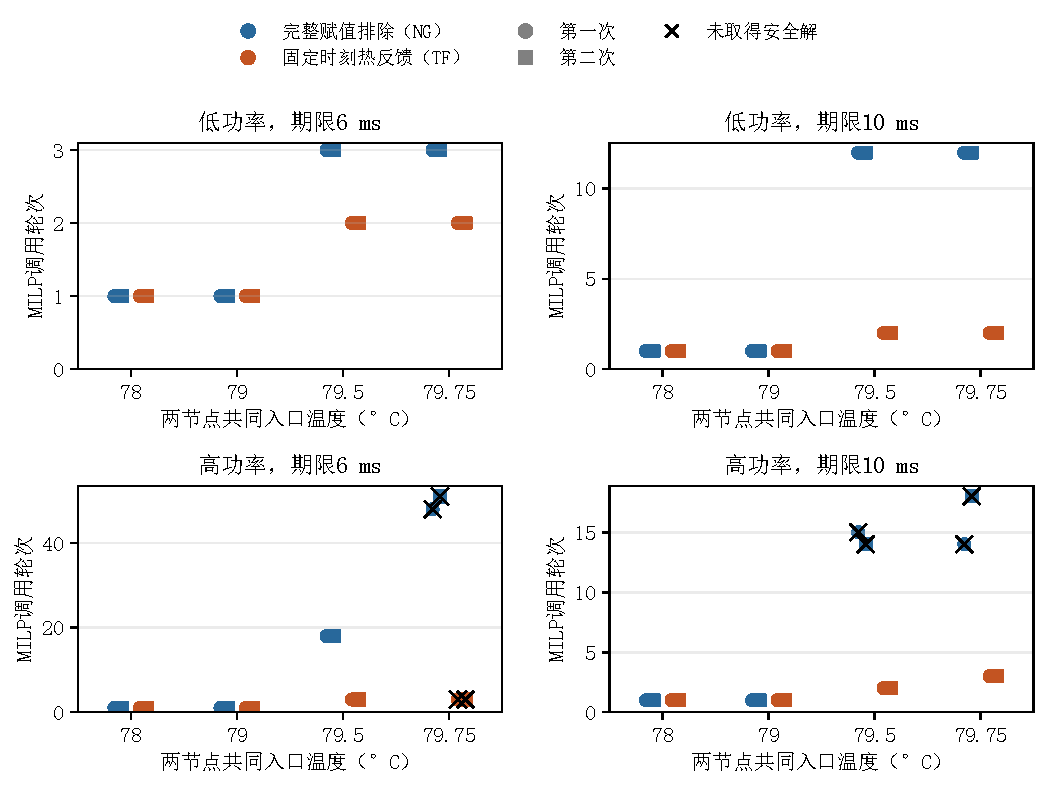
\includegraphics[width=\linewidth]{figures/pressure78_rounds.pdf}
\caption{预定入口热压力下两方法的MILP调用轮次。圆点、方点分别表示两次运行，叉号表示预算内没有安全输出；横向偏移只为避免遮挡。超时轮次是已发生的调用数，不表示搜索完成。各温度作为离散条件展示，不插值为连续区域边界。}
\label{fig:pressure-rounds}
\end{figure}

\clearpage

在每种方法的32次调用中，NG与TF分别取得26次和30次预算内安全输出，其中分别有12次和16次达到独立下界。双方均成功的26个配对所得能量全部相同，差异主要体现在安全输出次数与求解过程。低功率包79.5和79.75°C下的四个条件，以及高功率包6 ms、79.5°C条件，在两次运行中均减少求解轮次并缩短墙钟时间；其中，低功率包10 ms的两档高温条件均由12轮降至2轮。这五个条件下，两方法最终给出的时间表不同，说明相同能量仍可通过不同安全安排实现。

\begin{samepage}
高功率、10 ms、79.5与79.75°C两个条件中，NG四次调用均超时，未取得安全$U$；TF分别经过2轮和3轮取得42.625 mJ，并由$U=L_0$独立确定最优值。TF取得的安全见证同时确认了这些条件的可行性，NG则未能在本次预算内找到安全安排。这一差异体现的是有限预算下取得有效答案的能力；NG没有输出能量，因而这两个条件不能用于计算两方法之间的节能率。
\par
\end{samepage}

高功率、6 ms、79.75°C下，两方法均没有安全输出。NG两次超时；TF两次均加入两条热行，在完成3轮后由求解器报告无解。热行有效性保证安全安排得到保留，却不能独立认证浮点求解器已排尽剩余整数域。因此，该条件的结论仍为未取得安全输出与求解器报告无解，尚无独立热不可行证明；相应内部界和退出状态也与安全$U$、独立$L_0$分列报告。

较低入口提供了未触发反馈的对照。78与79°C的8个条件中，首候选均安全，两方法都只求解一轮且未执行反馈；对应16个配对中，TF恰有8次较快、8次较慢，这些时间差不能归因于未执行的热行。两档较高初温的8个条件中，首候选均违规；全部32个配对的首候选选项集合相同，排除了不同初始候选这一解释。两次顺序平衡运行支持本组观察的一致性，但不足以估计方差、置信区间或认定跨平台稳定加速。

求解过程进一步反映了两种反馈传递信息的差异。正式组中，NG共生成240条完整赋值排除，TF生成22条热行且无回退；累计求解轮次由272降至54，不同候选及完整热评价次数由282降至56。一轮求解可能在回调中访问多个候选，因而轮次与候选数分别统计。全部保存轮次的求解器分支节点计数均为0，减少的是外层重复求解，而非分支树节点。TF累计约束构造时间为0.602 s，高于NG的0.042 s；在触发反馈且双方成功的五个条件中，后续求解减少抵消了这项新增成本。

上述耗时采用完整调用的墙钟时间，首次取得安全输出的时间另以外部时刻区间记录，并以上端判断是否满足预算。NG六次超时调用实际在60.164--63.701 s返回，超出60 s的部分为停止延迟。完整墙钟保留了这一停止成本，预算内证据则仅接纳预算结束前完成检查的结果，未将晚形成的状态或内部界补记为有效输出；首次安全时间的区间下端也不作为精确首解时刻。

为检查已有违规轨迹能否在正常求解中触发反馈，另设高功率、6 ms、79.45°C的发现性诊断。该点依据既有轨迹构造，两方法各运行一次，均自主取得44 mJ安全输出：NG为18轮、24.826 s，TF为3轮、4.205 s。独立$L_0$仍为42.625 mJ，因此本项结果只提供安全见证与内部收敛。由于选点方式与正式温度组不同，诊断结果单独报告，不并入16个正式条件的成功率或重复统计。

离线检查表明，一条热行能够排除共享温度关系的多条违规安排；完整求解进一步表明，当较高入口使正常候选违规时，这种信息复用可以减少重复尝试，并在部分受预算限制的调用中取得安全最优值见证。该变化来自求解过程，能耗模型保持不变，双方均成功时也未观察到能量下降。结论适用于所列抽象参数、有限网格和求解器设置，不能据此推断真实设备节能或全部热调度实例的速度优势。


\subsection{结果讨论与适用范围}

本节结果分别回答了模型与方法的验证问题。任务响应修正的系统价值受期限和资源限制，温度约束可以收缩最优配置集合而不提高最低能量；在此模型上，连续温度违规信息能够形成有效线性约束，并在所测高入口条件下减少重复求解。表\ref{tab:evidence-map}汇总各项结论的求解来源和适用范围。

\begin{table}[htbp]
\centering\small
\caption{验证问题、求解来源与证据范围}\label{tab:evidence-map}
\setlength{\tabcolsep}{4pt}
\begin{tabular}{@{}p{2.2cm}p{2.5cm}p{4.4cm}p{4.7cm}@{}}
\toprule
验证问题 & 求解来源 & 已有证据 & 尚不能支持的结论\\
\midrule
响应修正是否改变决策 & 解析下界、排除及见证核验 & 宽期限有能量差，紧期限不变；覆盖反比模型并列解的回放能量 & 不是两种响应的MILP直接配对运行，也不是实测精度验证\\
温度是否限制配置 & 完整网格枚举 & 104个最优配置保留80个，最低仍44 mJ & 不推出最低能量提高或连续启动域的配置排除\\
热行是否利用更多信息 & 完整合法域离线核对 & 单行排除16或32条违规安排，零误删安全安排 & 排除数量本身不等于MILP加速\\
接入是否必然触发 & 原输入上独立MILP对照 & 9项可行输入均首轮安全，全部零反馈 & 不能由未触发时的耗时差判断反馈价值\\
反馈是否改善求解 & 16条件、两方法、两次运行 & 安全输出26/32与30/32；5条件轮次及时间减少，2条件仅反馈取得安全解 & 不证明普遍加速、运行能耗下降或创新充分成立\\
\bottomrule
\end{tabular}
\end{table}

本章方法将完整轨迹中已确认的违规节点与时刻转换为全部选项共同满足的温度必要条件，再通过可靠数值包络将其反馈给MILP。在线性热模型和约束生成思想的基础上，本章针对设备映射、频率与启动选项建立约束表达，论证有效性并验证求解表现。RC模型、查表和约束生成本身仍采用已有原理。与逐条删除当前安排相比，方法能否产生实际收益，取决于求解器是否遇到违规候选、不同候选是否共享温度关系，以及约束构造代价能否由后续求解减少抵消。

\begin{samepage}
各组输入、时间表、结果与求解来源的复现索引见随稿材料\cite{artifact-index}。其中，响应对照采用解析证据，尚未进行两种响应模型的MILP直接配对运行。第四章与有界搜索的比较应使用相同输入、预算和连续热接纳条件，并以加入热行反馈后的MILP为比较对象；此前针对完整赋值排除方法的比较不能替代这一检验。
\par\end{samepage}

本章结果的现实适用范围受参数来源限制。公开工件提供了四Stage结构及作者报告的设备支持，但目前缺少同平台Lite0各Stage的多频点时长、活动功率和配套RC测量。因此，实验分析的是声明条件下的决策关系，尚不能估计某款设备的实际节能率。冷热入口与期限对照也只覆盖所列条件，不能用于推断这些关系在现实系统中的出现频率。

能量分解的适用范围还取决于加性功率与固定模式响应。若并发改变活动功率或执行时长，或温度相关泄漏、休眠及切换代价使能量依赖具体安排，目标一般需恢复为$E(m,s)$。此时，一条安全时序不能确定整个配置的最低能量，独立Stage下界也须重新检查，尤其需要计入可能为负的并发修正。温度漏电与工作点保持已纳入第3.2—3.5节的一般模型，但其求解与验证不在本节结果范围内；并发残差、休眠和非零切换仍不属于本章基础假设。

\section{本章小结}

本章面向端侧协同多模型完整请求，建立设备、工作点与执行时序的热约束节能联合问题。合法模式提供任务相关代价，依赖、资源和共享域限定执行关系；功率按计量组去重，空闲工作点保持与温度漏电参与完整窗口能量。CPU固定单元及加速器设备的热状态通过耦合RC关联，完整安排的目标为\(E(m,s)\)。

在已实现的CPU--NPU恒功率特例上，本章保留有限网格MILP、连续热反馈及其验证。响应对照在宽期限下出现能量差，在紧期限下保留无变化条件；热约束收缩部分最优配置集合而未提高最低能量。预定热压力组中，安全输出由26/32次增至30/32次，共同成功时能量相同。这些结果对应原特例和输入，不替代一般模型的适配验证。

后续求解应围绕同一合法域与完整评价组织MILP参照和启发式，先处理工作点保持、漏电能量与多节点连续热检查的接口，再比较安全解质量和计算表现。

% 配置性质、热反馈推导与数值约定；在本章小结之后、符号索引之前载入。
\clearpage
\section*{补充性质与证明}
\label{sec:ch3-properties}
\markright{补充性质与证明}

本部分仅适用于第3.6—3.7节的恒功率、二聚合热节点特例；不将配置能量分解或固定选项热行推广为第3.2—3.5节一般模型的性质。

\subsection*{配置能量与时序可行性}

本部分说明配置能量与时序可行性的关系，并给出热约束影响最优配置及能耗的条件。模式中的映射与频率决定执行时长、活动能量、资源冲突和注热位置；时序决定这些选择能否组成满足全部要求的完整安排。两类决策的联系如图\ref{fig:config-timing}所示。

\begin{figure}[!htbp]
\centering
\resizebox{\linewidth}{!}{%
\begin{tikzpicture}[node distance=7mm and 10mm,box/.style={draw,rounded corners,align=center,text width=4.5cm,minimum height=10mm,font=\small},>=Latex]
\node[box] (d) {Stage模式表与合法支持};
\node[box,below=of d] (m) {配置$m$：执行单元与频率};
\node[box,below left=of m] (e) {固定配置能量$E(m)$};
\node[box,below right=of m] (s) {时序$s$：执行顺序与等待};
\node[box,below=of s] (r) {资源、频率域与请求期限};
\node[box,below=of e] (p) {配置与时序共同确定\par 完整节点功率轨迹$p(t)$};
\node[box,below=of p] (t) {入口状态与RC传播\par 连续热安全};
\node[box,below=of r] (f) {是否存在完整可行安排};
\node[box,below right=of t] (o) {选择最低可实现能量};
\draw[->] (d)--(m); \draw[->] (m)--(e); \draw[->] (m)--(s);
\draw[->] (s)--(r); \draw[->] (m.west) -| ([xshift=-4mm]p.west) -- (p.west);
\draw[->] (s)--(p); \draw[->] (p)--(t); \draw[->] (r)--(f);
\draw[->] (t)--(f); \draw[->] (f)--(o);
\draw[->] (e.west) -- ++(-10mm,0) |- (o.west);
\end{tikzpicture}%
}

\caption{配置能量与时序可行性的关系。图示为问题结构，不规定一次性的先配置后调度算法。}
\label{fig:config-timing}
\end{figure}

在上述特例的固定窗口、恒定基准功率、固定模式响应和零额外开销的条件下，每个Stage在窗口内完整执行一次，等待与重排不改变配置的总能量。因此，可以将“配置的代价是多少”与“该配置是否存在安全安排”分别描述。对固定配置\(m\)，记满足依赖、资源和期限等无热约束的启动向量集合为\(\mathcal S_0(m)\)，进一步满足温度约束的集合为\(\mathcal S_T(m)\)。存在相应时序的配置分别组成
\[
\mathcal M_0=\{m:\mathcal S_0(m)\ne\varnothing\},\qquad
\mathcal M_T=\{m:\mathcal S_T(m)\ne\varnothing\},
\]
\noindent\begin{minipage}{\linewidth}
\setlength{\parindent}{2em}
其中，所有配置均取自\(\prod_iM_i\)。以下集合与最优值均在相同启动域下比较。对于连续版本，时序集合允许连续起点；对于第\ref{sec:milp}节的网格版本，则统一限制到给定启动网格。联合问题可等价写为

\begin{equation}
\boxed{\min_{\substack{m\in\prod_{i\in V}M_i\\s\in\mathcal S_T(m)}}E(m)
=\min_{m\in\mathcal M_T}E(m).}
\label{eq:ch3-16}
\end{equation}

\textbf{命题3-1：} 式\eqref{eq:ch3-16}与联合问题具有相同的可实现目标值集合。

\textbf{证明：} 任意联合可行解\((m,s)\)中的配置都属于\(\mathcal M_T\)，能量为\(E(m)\)；反之，若\(m\in\mathcal M_T\)，则至少存在一条完整安全时序\(s\)，使\((m,s)\)成为联合可行解，能量同样为\(E(m)\)。两种表达取得的目标值集合因此相同。模式集合有限，\(\mathcal M_T\)非空时可取得其中最低能量；为空时则无完整可行安排。证毕。
\end{minipage}\par\medskip

该性质说明，找到一条满足全部约束的完整安排，就能证明其配置能量可以实现，即正文中所称的安全见证。一条时序失败则只排除了这一安排，判断整个配置不可行仍需覆盖其全部可能时序或给出充分排除依据。

温度要求对最优能耗的影响也可由此说明。设无热问题可行，其最优值为\(E_0^*=\min_{m\in\mathcal M_0}E(m)\)，最优配置集为\(\mathcal M_0^*=\{m\in\mathcal M_0:E(m)=E_0^*\}\)；若热问题也可行，记最优值为\(E_T^*\)。由于\(\mathcal M_T\subseteq\mathcal M_0\)，有

\begin{equation}
E_T^*\ge E_0^*,\qquad
E_T^*=E_0^*\ \Longleftrightarrow\ \mathcal M_T\cap\mathcal M_0^*\ne\varnothing.
\label{eq:ch3-17}
\end{equation}

只要原最优配置中还保留一个热可行配置，就能通过它的安全时序达到原最优值；反之，达到同一能量的热安全方案也必然来自这一交集。因此，最优配置集合缩小并不必然提高最低能耗。只有全部原最优配置被排除、但仍存在其他热可行配置时，有限配置集合才保证最优能量严格提高；若所有配置均被排除，则问题不可行。


\subsection*{选项热响应的展开}
\label{supp:option-response}

正文式\eqref{eq:thermal-affine}将节点温度分为基准与选项活动温升，此处给出各项的计算表达。在固定入口状态、线性时不变RC和可加活动功率下，每个选项的热响应可以分别独立计算。记全部选项为\(\mathcal O=\bigcup_{i\in V}\mathcal O_i\)，用热传播核描述温度状态随时间的变化：
\begin{equation}
K(t)=\exp(-C_{\rm th}^{-1}Gt),\qquad t\ge0.
\label{eq:thermal-kernel}
\end{equation}
温度基准由入口状态和持续的空闲注热产生，选项温升则由对应执行区间内的活动注热产生。设\(p^0=[p_C^0,p_N^0]^{\mathsf T}\)，\(\theta_0=\theta(0)\)。CPU模式选项\(o=(i,m,k)\)的活动注热向量为\(v_o=[Q_i(m),0]^{\mathsf T}\)，NPU模式则为\([0,Q_i(m)]^{\mathsf T}\)，单位均为W。边界外公共功率只计入系统能量，不进入\(p^0\)或\(v_o\)。由式\eqref{eq:ch3-14}，基准温度与选项响应分别为
\begin{equation}
\begin{aligned}
b_n(t)&=T_a+\left[K(t)\theta_0+
\int_0^t K(t-u)C_{\rm th}^{-1}p^0\,\mathrm du\right]_n,\\
h_{no}(t)&=
\begin{cases}
\displaystyle\left[\int_{t_o}^{\min(t,e_o)}
K(t-u)C_{\rm th}^{-1}v_o\,\mathrm du\right]_n,&t>t_o,\\
0,&t\le t_o.
\end{cases}
\end{aligned}
\label{eq:thermal-option-response}
\end{equation}
其中，\(b_n\)为包含初温和固定空闲注热的绝对温度，单位为°C；\(h_{no}\)为活动温升，单位为K，其数值可与°C温差相加。选项尚未启动时，活动温升为零；执行结束后，已有温升仍随热传播变化。因此，\(h_{no}\)同时取决于注热节点、执行区间和观察时刻，与只表示功率积分的活动能量\(\varepsilon_o\)承担不同作用。

本特例的被动RC网络中，\(-C_{\rm th}^{-1}G\)的非对角元素非负，因而\(K(t)\)逐元素非负；结合\(v_o\ge0\)，可得\(h_{no}(t)\ge0\)。上述系数依赖选项响应的独立性；若加入温度相关泄漏，或并发改变选项时长与功率，则需重新审查这种表达。


\subsection*{热反馈的有效性与覆盖关系}
\label{supp:feedback-properties}

将热演化与调度联合写入MILP已有研究基础。Pierson等采用离散时间热模型建立资源分配与能量优化约束\cite{pierson2020}；本章则在连续耦合RC模型下，依据完整轨迹的违规位置生成约束。有限主问题与违规分离交替进行的组织方式可借鉴Subramanyam等的研究\cite{subramanyam2020}，约束有效性及终止条件仍需按本问题的假设推导，其收敛结论不能直接移用。

正文中的反馈行采用响应下界与放宽右端，并对源候选验证严格分离。下面分别说明这两项条件所保证的安全保留与排除范围。

\noindent\begin{minipage}{\linewidth}
\setlength{\parindent}{2em}
\textbf{命题3-2：} 式\eqref{eq:thermal-safe-row}保留全部原热安全安排。

\textbf{证明：} 若安排违反该行，由\(y_o\ge0\)及响应下界可得
\begin{equation}
T_n(\bar t;y)\ge\underline b_n+\sum_o a_oy_o
>\underline b_n+r\ge T_n^{\max}+\epsilon_T.
\label{eq:thermal-row-validity}
\end{equation}
故被排除安排必然超温，不属于原热安全集合。放宽右端只会减小排除范围，不会改变最终安全接纳标准。\hfill$\square$
\end{minipage}\par\medskip

\textbf{命题3-3：} 在满足逐Stage唯一选择的合法整数域中，若式\eqref{eq:thermal-source-separation}成立，则热行保留的安排集合包含于对应完整赋值排除保留的集合。

\textbf{证明：} 完整赋值排除只删除同时选择\(J^*\)中全部\(N\)个选项的安排，唯一选择约束保证该安排就是源安排。式\eqref{eq:thermal-source-separation}保证源安排也被热行删除，故满足热行的整数安排必满足对应完整赋值排除。\hfill$\square$

只有存在另一个同样违反该热行的合法整数安排时，上述包含关系才严格。命题说明违规温度信息可以用于排除其他安排，其范围限于满足唯一选择约束的合法整数域；分数解上的支配关系及实际求解加速仍需分别研究。

上述两项条件也给出有限域内的终止依据。假设主问题精确求解，连续热判定能够按原温度约束将每个候选明确分为安全或违规，不存在未分辨状态；若每轮新增约束全域有效，并严格排除当前违规候选，该候选便不会再次出现。选项域有限，因此在预算不限时，反馈经过有限轮次必得到安全安排或排空合法域。进一步，若每轮返回当前松弛问题的真正最优解，首次被接纳的安全解就是原有限网格热问题的最优解：松弛最优值提供下界，该安全解提供相同的可行上界。

实际求解的停止结论还取决于数值判定与计算预算。响应系数和连续峰温包络的数值保证均限于已核对的对称二节点实现；一般RC线性关系本身不提供任意网络的数值认证。求解过程分别保存安全\(U\)、独立\(L_0\)、求解器内部界及未决状态，有效热行也不独立认证求解器内部界。因此，超时、未分辨或主问题未收敛时，结果仍按已取得的证据报告，不能由有限域终止论证推定搜索已经完成。


\subsection*{数值复核与实现约定}
\label{supp:numerical-checks}
\enlargethispage{\baselineskip}

峰温误差包络与判定带宽承担不同作用：前者控制峰温计算误差，后者区分接近阈值的情况。对系数、右端与求和也需分别采用可靠包络，不能仅将温度容差视作计算误差保证。式\eqref{eq:thermal-safe-row}采用非负响应下界，放宽右端会减小排除范围，但不改变最终安全接纳标准。

完整轨迹已证违规后，名义峰时刻只用于定位。实现需在具体可表示时刻重新构造点证书，并对源候选的被选集合\(J^*\)计算可靠求和下界，验证式\eqref{eq:thermal-source-separation}。全局峰温下界不能代替某个时刻的点温度下界，普通浮点和略大于右端也不能作为严格分离证据。完整轨迹违规但点证书或分离条件未成立时，回退式\eqref{eq:no-good}；轨迹未分辨时，两种排除均不生成。

检查器先按指定整数容差解码近整数候选，再根据真实区间复核唯一选择、依赖、资源和频率域要求。整数结构约束与浮点热行分开检查，热行采用可靠区间求和。解码或结构复核失败记为数值异常，不接纳候选，也不据此生成热排除。

一次调用按完整选项集合识别缓存候选，可复用完全相同候选的热检查结果；加入新热行后，仍需重新检查其是否满足当前约束。热行按完整系数向量及右端的精确相等识别重复，只保留一条。重复行不构成新进展；再次返回已被热行明确排除的违规候选时，记录容差事件并改用该完整赋值的排除。若候选还违反已加入的整数排除约束，则停止为数值异常，不反复重启。

热行检查与完整轨迹检查保持一致：热行比较未分辨、完整轨迹已证安全时，可依据完整检查保存安全\(U\)；若达到\(U=L_0\)，仍可独立证明最优值。未达到独立上下界闭合且最终热行比较仍未分辨时，停止为数值未决。热行明确违规而完整轨迹被判安全时，记录矛盾并停止为异常。实现错误不作为正常回退处理。

有限网格的安全安排也是连续启动问题的安全安排；网格最优或不可行结论则限于该受限域。只有连续域有效下界被某个网格安全安排达到时，才能进一步确定连续域最优值。\(L_0\)的独立Stage构造对两种域均成立，使用时仍须确认各模式集非空，并区分最优值与全部最优配置集合。


% 当前多场景模型的章末索引。
\clearpage
\section*{本章符号索引}
\markright{本章符号索引}

各符号在正文首次使用处定义。本表按输入、决策与派生量归类，内部时间、频率、功率和能量单位分别为s、Hz、W和J；温度使用摄氏温标，温差使用K。

\begin{longtable}{@{}p{5.1cm}p{6.1cm}>{\raggedright\arraybackslash}p{2.8cm}@{}}
\caption{多场景联合规划的主要符号}\label{tab:symbols}\\
\toprule
符号 & 含义 & 类型／单位 \\
\midrule
\endfirsthead
\toprule
符号 & 含义 & 类型／单位 \\
\midrule
\endhead
\(\mathcal A,G_a,V_a,E_a\) & 应用及其固定Stage工作流 & 输入集合／图 \\
\(\mathcal C,\mathcal R_c,\mathcal I_c,\mathcal E_c\) & 场景、请求、Stage实例及依赖 & 输入集合 \\
\(\mathcal J,\tau(c,i),r(c,i),\mathcal O_{cr}\) & 固定Stage身份、实例归属及必需输出 & 输入集合／映射 \\
\(r_{cr},d^{\rm rel}_{cr},D_{cr},W_c\) & 释放、相对期限、绝对期限及窗口 & 输入，s \\
\(p_c\) & 完整场景片段的次数权重 & 输入，无量纲 \\
\(\mathcal U_C,\mathcal U_G,\mathcal U_N\) & CPU固定单元、GPU及NPU设备 & 输入集合 \\
\(\mathcal H,\gamma(u),\mathcal K_h\) & 控制域、单元归属及合法工作点 & 输入集合／映射 \\
\(f_h(k),v_h(k),k^0_{ch}\) & 工作点频率、电压及入口状态 & Hz、V、状态标签 \\
\(\mathcal M_{ci},u(m),\kappa(m)\) & 合法模式、对应单元及完整域工作点 & 输入集合／映射 \\
\(d^{\rm ref}_{\tau u},f^{\rm ref}_u,\alpha_{\tau u}\) & 参考时长、参考频率及可缩放比例 & s、Hz、无量纲 \\
\(d_\tau(m),q_\tau(m)\) & 模式时长及活动增量功率 & 派生／输入，s、W \\
\(\mathcal B,\pi(u),\xi_{cg}(t)\) & 计量组、单元归属及组控制状态 & 输入／派生 \\
\(B_g,\lambda_{gn},T_g^{\rm ref}\) & 参考基准、本地温度系数及参考温度 & W、W/K、摄氏度 \\
\(a^B_{ng},n(u),h_{nu}\) & 基准分布、单元节点及活动注热映射 & 输入，无量纲／映射 \\
\(\mathcal N,C,G,T_a,T_c^0,T_n^{\max}\) & 热节点、热容、导热及温度输入 & J/K、W/K、摄氏度 \\
\(P_{{\rm ext},c},E_{{\rm ext},c}\) & 给定边界外功率及其窗口能量 & W、J \\
\midrule
\(u_\tau,m_{ci},s_{ci}\) & 共享部署、实例模式及启动时刻 & 共同／场景内决策 \\
\(F_{ci},I_{ci},\iota_{ci},k_{ch}(t)\) & 完成、执行区间、活动及域轨迹 & 派生，s／0--1／标签 \\
\(P_{cg},p^{\rm heat}_{cn},\theta_c,E_c,\bar E\) & 组电功率、注热、温升及能量 & W、K、J \\
\midrule
\(\mathcal G_{cim},\mathcal Q_{ci},\mathcal Q_c\) & 有限启动集合与单Stage选项 & 输入／派生集合 \\
\(t_o,f_o,d_o,q_o,u_o,h_o,\kappa_o\) & 选项的起止、代价及资源控制要求 & 已知选项参数 \\
\(e_{c\ell},\delta_{c\ell},\chi_{co\ell}\) & 固定事件、片长及半开区间覆盖 & 已知，s、0/1 \\
\(x_{\tau u},y_{co}\) & 共享部署和选项选择 & 二元变量 \\
\(\rho_{ch\ell k},w_{c\ell\omega}\) & 域状态及相容联合状态选择 & 二元辅助变量 \\
\(\Omega,J_{ch\ell},v_{c\ell}\) & 联合状态集、新启动数量及活动向量 & 输入／派生 \\
\(\theta_{c\ell},\Delta E_{c\ell}\) & 事件温升及完整段能量 & 连续变量，K、J \\
\(A_\omega,b_\omega,D_c,\beta_\omega,\ell_\omega\) & 固定状态下的热与电功率系数 & 由物理输入派生 \\
\(\Phi,\psi,\Gamma,\mu,\zeta,\nu\) & 温度传播及能量积分系数 & 由状态／片长派生 \\
\(H_c,\overline P_c,M^T,M^E\) & 状态、功率及条件行残差界 & 有依据的派生界 \\
\(\mathcal H^{(j)},U\) & 已加入的必要行及安全能量上界 & 求解记录，J \\
\bottomrule
\end{longtable}

 合入后续学校模板。
\documentclass[UTF8,a4paper,12pt,openany,fontset=windows]{ctexbook}
\usepackage[margin=25mm]{geometry}
\usepackage{amsmath,amssymb,mathtools}
\usepackage{booktabs,longtable,array,calc}
\usepackage{graphicx,tikz}
\usetikzlibrary{positioning,arrows.meta}
\usepackage[hidelinks,unicode]{hyperref}
\usepackage{xurl}
\providecommand{\tightlist}{\setlength{\itemsep}{0pt}\setlength{\parskip}{0pt}}
\setlength{\emergencystretch}{3em}
\renewcommand{\topfraction}{0.9}
\renewcommand{\bottomfraction}{0.8}
\renewcommand{\textfraction}{0.08}
\renewcommand{\floatpagefraction}{0.8}
\setcounter{topnumber}{3}
\setcounter{totalnumber}{4}
\renewcommand{\arraystretch}{1.25}
\renewcommand{\theequation}{\thechapter-\arabic{equation}}
\renewcommand{\thefigure}{\thechapter-\arabic{figure}}
\renewcommand{\thetable}{\thechapter-\arabic{table}}
\ctexset{chapter={format=\centering\Large\bfseries},section={format=\large\bfseries}}
\begin{document}
\setcounter{chapter}{2}
% 第三章正文主版本；历史Markdown不再同步。
\chapter[端侧协同推理的热约束节能调度建模与求解]{端侧协同推理的热约束\\节能调度建模与求解}
\label{chap:model}

\section{本章引言}

本章研究端侧协同多模型完整请求的热约束节能调度。一次请求可以包含前处理、多个模型分支及共同后继，只有全部必需输出完成才算完成。部署到CPU、GPU和NPU平台后，分支可以利用不同资源并行执行，也可能因竞争同一设备而排队。因此，需要共同决定各Stage使用的设备、工作点和启动时刻，在期限与温度约束下降低系统总能耗。

局部执行效率并不能独立决定完整请求的代价。降低某个分支的频率会改变资源占用和汇合时刻，调整次序或等待又会改变后继的入口热状态。已有热调度研究通过映射、频率及时间余量协调能耗与温度\cite{source1,li2019}。本章沿用这一联合分析思路，以逐Stage响应表示不同执行选择，并将共享频率域、空闲工作点保持和温度漏电放在完整请求的时间轴上评价。

本章先建立一般问题，再保留已实现的恒功率特例及其条件性验证。在该特例上，连续热约束反馈混合整数线性规划方法（Continuous Thermal Feedback-based Mixed Integer Linear Programming，CTF-MILP）以有限网格产生候选安排，检查完整温度轨迹，并将已确认的违规信息反馈给主问题。一般模型还包含工作点保持和温度功率反馈，下文分别说明其数学关系及与已有实现的衔接。

本章结构如下：第3.2节介绍任务、处理器和执行模式，明确调度对象与执行代价；第3.3节建立功耗与温度模型；第3.4节给出问题定义；第3.5节按约束与目标建立联合问题；第3.6节介绍恒功率特例上的CTF-MILP及其求解流程；第3.7节通过仿真分析响应修正的决策影响与热反馈的求解效果；第3.8节总结本章工作。

\section{系统模型}

一个调度方案需要回答三个问题：哪些计算必须完成，可使用哪些处理器，以及每种执行选择需要多少时间和功率。本节据此建立任务模型、处理器模型和执行模式，为后续约束与优化目标提供输入。

\subsection{任务模型}

多模型推理需要先明确一次服务何时完成。若两个模型分别产生所需结果，服务需等待两者均完成；若一个模型使用另一个模型的输出，则还需按数据依赖完成相应调用。本文用工作流描述参与调用的模型及其输入输出关系，将工作流的一次调用称为一个请求。一个请求可以包含一个或多个模型调用，所需输出全部产生后才算完成。本章在规划前确定模型、输入规格、精度和工作流结构，调度器据此选择执行设备、频率与时序。

为了安排模型内部的计算，本文将一组在同一执行单元上连续完成的算子作为一个计算阶段，记为Stage。每个模型依据执行后端的支持条件划分为若干Stage，划分在规划前确定，每个Stage实例执行一次。沿用第二章的DAG表示，将模型内部的Stage依赖与模型之间的输入输出依赖连接起来，就得到一次请求的完整任务图。工作流可以包含不同数量的模型，各模型的Stage数量由其结构与划分决定。

设本次参与规划的有限请求集合为\(\mathcal R\)。请求\(r\)的任务图表示为
\[
G_r=(V_r,A_r),
\]
其中，\(V_r\)是该请求的非空Stage集合，\(A_r\)是数据依赖边集合。若\((i,j)\in A_r\)，则Stage \(j\)需要等待Stage \(i\)的输出准备完成后才能开始。任务图为有向无环图，允许链式、分支及汇合等结构。不同请求的Stage实例集合互不相交，即使调用相同模型，也各自占用执行时间和计算资源。记全部Stage与依赖边为
\[
V=\bigcup_{r\in\mathcal R}V_r,\qquad
A=\bigcup_{r\in\mathcal R}A_r,
\]
并以\(r(i)\)表示Stage \(i\)所属请求。

请求的时间要求由到达时间\(a_r\)和绝对截止时间\(D_r\)给出：属于该请求的Stage只能在到达后执行，并须在截止时间之前产生全部所需输出。本文采用执行前规划，本次优化中的请求集合、到达时间和期限均预先给定。为在相同时间范围内比较调度方案，系统能耗与温度统一在窗口\([0,W]\)内评价，且\(0\le a_r<D_r\le W\)，使窗口覆盖所有请求的期限。

图\ref{fig:stage-structure}以第3.7节保留的单模型链式特例说明Stage级表示。该实例采用Band作者仓库中EfficientDet-Lite0的四组算子划分及设备支持信息\cite{source3,source4,source5}。S0、S1、S2和S3依次执行，其中S1可以映射到CPU或该工件报告支持的NPU，其余阶段在本章实例中使用CPU。整个请求在S3完成时结束。表\ref{tab:stage-support}列出相应算子范围。

\begin{figure}[htbp]
\centering
\begin{tikzpicture}[node distance=5mm,box/.style={draw,rounded corners,align=center,text width=8cm,minimum height=8mm,font=\small},>=Latex]
\node[box] (i) {模型输入：$1\times320\times320\times3$，UINT8};
\node[box,below=of i] (s0) {S0：CPU，算子0};
\node[box,below=of s0] (s1) {S1：CPU或指定NPU，算子1--65};
\node[box,below=of s1] (s2) {S2：CPU，算子66--265};
\node[box,below=of s2] (s3) {S3：CPU，算子266};
\node[box,below=of s3] (o) {模型输出};
\foreach \a/\b in {i/s0,s0/s1,s1/s2,s2/s3,s3/o} \draw[->] (\a)--(\b);
\end{tikzpicture}
\caption{单模型请求的四Stage实例。箭头表示数据依赖，完整请求在S3产生最终输出后完成。}
\label{fig:stage-structure}
\end{figure}

\begin{table}[htbp]
\centering\small
\caption{四Stage实例的算子划分与设备支持}\label{tab:stage-support}
\begin{tabular}{@{}p{1.3cm}p{2.9cm}p{4.5cm}p{4.1cm}@{}}
\toprule
Stage & 算子范围（含端点） & 本实例可用执行设备 & 请求中的作用 \\
\midrule
S0 & 0 & CPU & 首阶段 \\
S1 & 1--65 & CPU、工件所支持的NPU & 可选择执行设备 \\
S2 & 66--265 & CPU & 处理S1的输出 \\
S3 & 266 & CPU & 产生最终输出 \\
\bottomrule
\end{tabular}
\end{table}

第3.7节的历史实验采用该单模型工作流的两个调用，其时长、功率及热参数按该节条件给出。该图说明Stage与合法支持的表达，不限定一般协同工作流的分支结构、请求数量或资源数量。

\subsection{处理器模型}

平台包含CPU、GPU和NPU三类资源，执行单元集合分别记为\(\mathcal U_C\)、\(\mathcal U_G\)和\(\mathcal U_N\)，并令\(\mathcal U=\mathcal U_C\cup\mathcal U_G\cup\mathcal U_N\)。CPU单元可以是一颗核或一个固定核组，各单元的占核集合互不重叠，线程数和亲和性预先确定。GPU与NPU采用设备级映射，内部计算并行体现在阶段响应中。资源数量由具体平台给出，每个执行单元同一时刻只执行一个Stage，不同单元可以并发。

处理器通过合法的电压--频率工作点运行。设频率控制域集合为\(\mathcal D\)，\(h(u)\)为单元\(u\)所属的域，\(\mathcal K_\delta\)为域\(\delta\)的合法工作点集合。一个工作点\(k\)给出相应频率\(f_\delta(k)\)和电压\(v_\delta(k)\)，二者作为配套输入，不独立优化。具有独立控制权限的GPU或NPU对应自己的域；采用固定服务方式的设备，其工作点集合只有一个元素。域划分和可控制范围由平台输入确定。

同一CPU域内的执行单元共享频率，因此并发Stage必须采用相容的同一域工作点。本文规定域内有Stage执行时不切换工作点；上一忙段全部结束后，下一忙段可以采用新的合法工作点。Stage在执行中不可抢占、迁移或改点。尚未启动的Stage则可在规划中改选模式、调整次序或等待，以协调资源、期限和热状态。

空闲期间也需要确定设备的控制状态。记\(k_\delta^0\)为窗口入口工作点，\(k_\delta(t)\)为时刻\(t\)的域状态。首次工作开始前保持\(k_\delta^0\)，两次忙段之间及最后一次完成后的尾段保持上一忙段工作点，只在新的忙段开始时按需切换。因此，\(k_\delta(t)\)由完整安排和入口状态导出，不是可在空闲时任意改变的附加变量。本文将额外交接、搬运、格式转换及切换的时间和能量设为零；所需前后处理和回退计算仍保留在任务图或合法模式的计算范围中。

\subsection{执行模式}

执行设备和工作点共同决定Stage的资源占用及执行代价。本文将二者的组合称为执行模式，Stage \(i\)的全部合法模式组成有限集合\(M_i\)。模式\(m\in M_i\)给出执行单元\(u(m)\)、域工作点\(k(m)\in\mathcal K_{h(u(m))}\)、时长\(d_i(m)>0\)和活动增量功率\(Q_i(m)\ge0\)，单位分别为s和W。只有后端完整支持该Stage、资源及控制条件匹配的组合才进入\(M_i\)。

模式表按Stage、执行单元与工作点分别提供响应。对相同工作量和配置使用一致参数，本文采用的时长及活动增量不随并发组合或温度改变；温度对漏电的影响在下一节单独计入。参数可以来自匹配测量或明确给定的响应模型，采用何种统计口径及执行条件需要随输入记录。调度器选择模式时，选择的是一组已知代价，而非重新拟合响应函数。

不同Stage降频后的时长增幅可以不同。为说明这一关系，在一个给定CPU单元上，以\(F_{\rm ref}\)为参考频率、\(\bar d_i\)为参考时长，令\(x=f/F_{\rm ref}>0\)。统一反比刻画与一种任务相关刻画分别为
\begin{equation}
\widehat d_i^I(x)=\frac{\bar d_i}{x},\qquad
\widehat d_i^R(x)=\bar d_i\left[(1-\alpha_i)+\frac{\alpha_i}{x}\right],\quad 0\le\alpha_i\le1.
\label{eq:ch3-1}
\end{equation}
其中，\(\alpha_i\)表示参考时长中随频率反比缩放的比例。Zhou等采用固定周期数对应的反比时长\cite{source1}；本文允许逐Stage响应，式\eqref{eq:ch3-1}是后文条件对照采用的参数形式。逐模式给出的时长也可直接进入一般模型，无须服从这一公式。

例如，频率减半时，\(\alpha_i=1\)和\(\alpha_i=0.5\)分别对应两倍和1.5倍参考时长。这样的差异影响降频需要占用多少时间，而其系统能耗价值仍需结合后继、其他请求及温度评价。全部模式选择记为\(m=(m_i)_{i\in V}\)，启动向量记为\(s=(s_i)_{i\in V}\)。两者组成完整安排，确定各Stage的完成时刻、半开执行区间和运行指示：
\begin{equation}
b_i=s_i+d_i(m_i),\qquad I_i=[s_i,b_i),\qquad z_i(t)=\mathbf1_{I_i}(t).
\label{eq:ch3-2}
\end{equation}
半开区间允许一个Stage结束时另一个立即开始。模式和起点确定后，执行顺序、并发、等待及域工作点保持过程随之确定，为功率和温度评价提供完整时间轴。

\section{功耗与温度模型}

阶段响应说明每项计算需要多少时间和活动功率，系统评价还需计入设备空闲及温度变化。本节先说明功耗分解，再分别讨论CPU、GPU和NPU的计量关系，最后将完整安排转化为系统能耗与连续温度轨迹。

\subsection{功耗分解与运行状态}

处理器动态功耗主要来自电路充放电，静态功耗主要包括器件漏电。常用CMOS近似将两者写为\cite{source1,wang2025dvfs}
\begin{equation}
P_{\rm dyn}\approx aC^{\rm eff}v^2f,\qquad P_{\rm leak}=vI_{\rm leak}(v,T).
\label{eq:power-physical}
\end{equation}
其中，\(a\)为开关活动因子，\(C^{\rm eff}\)为等效电容，\(v\)为电压，\(f\)为频率，\(I_{\rm leak}\)为漏电流。改变合法工作点会改变电压、频率及执行时长；温度则进一步影响漏电。CPU、GPU和NPU具有共同的物理分解，但相应参数由设备与负载分别确定。

为由时间表计算功率，本文区分工作态和空闲态，并采用“持续基准＋Stage活动增量”的计量方式。空闲时仍存在控制电路活动和漏电，故空闲功率并非仅指静态功率。不同执行单元也可能共享部分电路，不能对每个并发Stage重复计入同一公共基准。

记\(\mathcal P\)为互不重叠的功率计量组集合，\(\pi(u)\)为单元\(u\)所属组。计量组与频率域分别描述计量边界和控制关系，二者不必一一对应。以\(\kappa_p(t)\)表示影响组\(p\)功耗的域工作点组合；组只涉及一个域时，它就是该域工作点。记\(\bar T_p(t)\)为组功耗采用的代表温度。在参考温度\(T_p^{\rm ref}\)附近，以局部线性漏电刻画空闲基准：
\begin{equation}
P_p^{\rm idle}(t)=B_p(\kappa_p(t))+\lambda_p(\kappa_p(t))\bigl[\bar T_p(t)-T_p^{\rm ref}\bigr].
\label{eq:r86-idle}
\end{equation}
\(B_p\)是参考温度下的基准功率，单位为W；\(\lambda_p\)是温度系数，单位为W/K。系数按计量组和工作点给定，工作与空闲使用同一系数，不为每个Stage另设漏电斜率。局部线性温度功率关系可见Li等的处理器模型及F-DTM的设备模型\cite{li2019,fdtm2022}。本文在输入声明的有效温区内使用该关系，并要求功率非负。

在相同工作点及温度下，Stage执行增加的功率由\(Q_i(m_i)\)表示。该增量与式\eqref{eq:r86-idle}相加，而不是再计入一份完整设备功率。这样既保留任务活动差异，也能沿同一时间轴计算工作和空闲时的温度漏电。

\subsection{CPU功耗模型}

CPU的多个固定执行单元可以并行工作，组基准只计一次，活动增量按正在运行的Stage求和。对CPU计量组\(p\in\mathcal P_C\)，有
\begin{equation}
P_p(t)=P_p^{\rm idle}(t)+
\sum_{i:\,\pi(u(m_i))=p}Q_i(m_i)z_i(t).
\label{eq:cpu-power-model}
\end{equation}
其中，\(\mathcal P_C\)表示CPU计量组集合。\(Q_i(m)\)可由同工作点下工作功率与基准之差取得，也可用任务新增开关活动对应的\(\Delta a_{i,u}C_u^{\rm eff}v^2f\)近似参数化。后一表达解释DVFS与任务活动的来源，实际调度使用模式表中的增量值。

共享频率域限制并发Stage可采用的工作点，但不把不同CPU单元的温度合为同一个数。各单元的活动功率注入对应热位置，共享基准及漏电按给定分配关系注入。于是，共享控制、基准去重和单元温度差异可以同时保留。

\subsection{GPU功耗模型}

GPU以设备作为可调度单元，设备内部大量计算单元的活动汇总到Stage响应中。本研究对每台GPU采用独占提交政策，因此同一时刻至多有一个Stage的活动增量计入该设备。设\(u\in\mathcal U_G\)，其增量为
\begin{equation}
P_u^{\rm inc}(t)=\sum_{i:\,u(m_i)=u}Q_i(m_i)z_i(t).
\label{eq:gpu-power-model}
\end{equation}
设备基准由所属计量组计入。若该GPU单独形成一个计量组，总功率就是组基准与式\eqref{eq:gpu-power-model}之和；若存在共享计量边界，则先按该边界去重后汇总。

不同Stage对GPU计算单元和存储通路的使用不同，可用活动因子或工作点下的参考增量进行参数化，最终均归入\(Q_i(m)\)。GPU的合法工作点及其Stage时长分别作为输入，不由CPU的频率响应推算。F-DTM采用按配置记录内核时长、按频率描述设备温度功率的方式\cite{fdtm2022}，为这种分开提供时长与功率参数的组织提供参考。

\subsection{NPU功耗模型}

NPU同样采用设备级映射，但Stage是否可执行还取决于后端对其完整算子范围的支持。支持调频的设备提供多个合法工作点，固定服务模式则只提供一个。设备的内部并行和不同算子活动均体现在\(d_i(m)\)与\(Q_i(m)\)中，不把内部计算核心展开为独立调度资源。

Wang等将AI加速器功率分为负载无关动态项、活动项及温度漏电项\cite{wang2025dvfs}。在单设备计量边界下，可用下式说明它与本文输入的对应：
\begin{equation}
\begin{aligned}
B_p(k)&=\beta_p f(k)v(k)^2+\ell_p v(k),\\
Q_i(m)&=\eta_{i,u}(k)f(k)v(k)^2,\qquad
\lambda_p(k)=\gamma_p(k)v(k).
\end{aligned}
\label{eq:npu-power-model}
\end{equation}
\(\beta_p\)和\(\eta_{i,u}\)表示等效开关系数，\(\ell_p\)为参考温度下漏电流，\(\gamma_p\)为其温度斜率。这是形成模式功率参数的一种方式，与CPU、GPU的“基准＋活动增量＋温度项”含义一致；不同设备采用各自参数，并不共用同一条拟合曲线。该文的数据来自其AI加速器平台，本文实例的参数来源需另行给出。

\subsection{统一功率与能耗表达}

将各计量组的基准与运行Stage的活动增量相加，得到完整系统功率。设\(P_{\rm ext}\ge0\)为计入系统能耗、位于所建热网络之外的恒定公共功率，则
\begin{equation}
\begin{aligned}
P_{\rm sys}(t;m,s)&=P_{\rm ext}+\sum_{p\in\mathcal P}P_p^{\rm idle}(t)
+\sum_{i\in V}Q_i(m_i)z_i(t),\\
E(m,s)&=\int_0^W P_{\rm sys}(t;m,s)\,\mathrm dt.
\end{aligned}
\label{eq:power-general-system}
\end{equation}
计量组覆盖所有纳入模型的设备基准，公共功率不再包含这些已计项目。本文采用固定响应和可加活动增量，不另设并发功率残差。由于每个Stage在窗口内完整执行一次，能量还可展开为
\begin{equation}
\begin{aligned}
E(m,s)={}&P_{\rm ext}W+\sum_{i\in V}Q_i(m_i)d_i(m_i)\\
&+\sum_{p\in\mathcal P}\int_0^W
\left\{B_p(\kappa_p(t))+\lambda_p(\kappa_p(t))
[\bar T_p(t)-T_p^{\rm ref}]\right\}\,\mathrm dt.
\end{aligned}
\label{eq:r86-energy}
\end{equation}
各Stage的活动能量由模式决定。参考基准\(B_p\)的积分取决于各工作点保持多久，漏电修正的积分则同时取决于工作点和温度轨迹。同一配置采用不同次序或等待，可能改变这两类积分，而不改变各Stage的活动能量，因此完整安排的能量一般记为\(E(m,s)\)。等待期间及全部请求完成后，活动增量可以为零，但设备仍保持工作点并持续消耗基准和漏电功率，均计入固定窗口。

\subsection{瞬态温度模型}

功率给出热量产生的速率，温度还受已有储热和散热过程影响。本文采用耦合热阻热容网络描述这一过程，热节点集合记为\(\mathcal N\)。CPU按固定执行单元区分热状态，GPU和NPU按设备级表示，并可设置与物理边界匹配的共享节点。固定核组节点表示该组的代表温度。Li等的耦合RC方程和F-DTM的CPU--GPU热模型提供了设备间传热及状态传播的参考\cite{li2019,fdtm2022}。

功率计量与空间注热需要通过明确映射衔接。设\(w_{np}\)为组\(p\)的基准及漏电注入节点\(n\)的比例，\(v_{nu}\)为单元\(u\)活动增量注入节点\(n\)的比例，两者非负且各列之和为1。组代表温度由输入映射\(H\)确定，\(\bar T_p(t)=\sum_n H_{pn}T_n(t)\)，其中\(H_{pn}\ge0\)、\(\sum_nH_{pn}=1\)；单节点代表是该映射的特例。三种映射分别回答在哪里发热和用哪个温度计算漏电，须依据匹配数据或明确的仿真设定给出。节点注热为
\begin{equation}
p_n(t)=\sum_{p\in\mathcal P}w_{np}P_p^{\rm idle}(t)
+\sum_{i\in V}v_{n,u(m_i)}Q_i(m_i)z_i(t).
\label{eq:r86-injection}
\end{equation}
由归一化条件，\(\sum_n p_n=P_{\rm sys}-P_{\rm ext}\)，同一功率不被重复注入。CPU单元的活动注热对应其声明的空间边界；计量组可包含多个热状态，而不强制各单元温度相同。\(P_{\rm ext}\)位于热边界之外，只进入能耗。

设环境温度\(T_a\)固定，\(\theta_n=T_n-T_a\)为温升，\(C_{\rm th}=\operatorname{diag}(C_n)\)为热容矩阵。令\(g_{nj}=g_{jn}\ge0\)为节点间导热、\(g_{na}\ge0\)为对环境导热，并定义\(G_{nn}=g_{na}+\sum_{j\ne n}g_{nj}\)、\(G_{nj}=-g_{nj}\)。要求\(C_n>0\)，各连通分量均连接环境，使无漏电反馈的RC网络被动且稳定。入口温度\(T_n^0\)给定，热平衡满足
\begin{equation}
C_{\rm th}\dot\theta(t)=-G\theta(t)+p(t),\qquad
\theta_n(0)=T_n^0-T_a,\quad n\in\mathcal N.
\label{eq:r86-thermal}
\end{equation}
热容、导热和功率的单位分别为J/K、W/K和W，方程两侧均为功率。入口不含未完成Stage，但保留此前运行造成的热状态。

温度漏电使注热也依赖温度。在相邻启动、结束及工作点切换事件之间，工作点组合\(\kappa\)和活动集合固定。将\(w_{np}\)组成矩阵\(S\)，将\(\lambda_p(\kappa_p)\)组成对角矩阵\(\Lambda_\kappa\)，有
\begin{equation}
\begin{aligned}
\dot\theta&=A_\kappa\theta+b_\kappa,\\
A_\kappa&=C_{\rm th}^{-1}(-G+S\Lambda_\kappa H),\\
b_\kappa&=C_{\rm th}^{-1}\left\{S[B_\kappa+\Lambda_\kappa(T_a\mathbf1-T^{\rm ref})]+q\right\}.
\end{aligned}
\label{eq:r86-state}
\end{equation}
这里，\(B_\kappa\)和\(T^{\rm ref}\)为各组参数向量，\(q_n=\sum_i v_{n,u(m_i)}Q_i(m_i)z_i\)为本段活动注热。\(b_\kappa\)同时取决于本段活动集合。物理RC不变，但工作点改变漏电系数时，等效状态矩阵也可能变化。参数输入须核对有效温区、非负功率及漏电反馈后的稳定性，不能只以被动RC代替该检查。

长度为\(\tau\)的事件段可按下式传播，并在事件边界保持温度连续：
\begin{equation}
\theta(t_0+\tau)=e^{A_\kappa\tau}\theta(t_0)
+\int_0^\tau e^{A_\kappa(\tau-\xi)}b_\kappa\,\mathrm d\xi.
\label{eq:r86-propagation}
\end{equation}
等待和空闲尾段使用同一方程，只有活动集合变化。完整热评价覆盖\([0,W]\)内的峰值，包括事件端点与段内极值；启动格点不能代替连续温度检查。节点上限约束在第3.5节给出，安全范围截至窗口末端。

\section{问题定义}
\label{sec:problem-definition}

基于前述模型，本文研究端侧协同多模型完整请求的热约束节能联合规划。输入包括有限已知请求及其DAG、到达和绝对期限，CPU、GPU和NPU执行单元及控制域，各Stage合法模式与响应，以及功率计量、入口状态、耦合RC和评价窗口。模型、输入规格、精度、Stage划分及必需输出均已给定。

规划需要共同确定每个Stage的执行模式\(m_i\)和启动时刻\(s_i\)。设备及工作点改变执行代价和资源占用，起点决定并发、排队和等待，二者还决定后续热状态与漏电能量。目标是在满足依赖、资源、控制域、完整请求期限和连续温度限制的安排中，使固定窗口系统能耗\(E(m,s)\)最低。完成时间和峰温在此分别用于期限与热安全约束，不另作优化目标。

一般问题采用连续启动时刻。为了限定后续计算域，也可给定网格间隔\(\Delta>0\)，只允许\(s_i\)取非负整数倍\(\Delta\)。这仅限制起点，\(d_i(m_i)\)和\(b_i\)仍取原值。网格安全解同时是连续域可行解，网格最优值是连续问题最优值的上界；网格无解不排除其他连续起点。具体网格和窗口由实例声明，不由一般模型预先取定。

\section{问题分析与形式化}
\label{sec:formal-model}

为建立上述问题，先选择Stage的合法模式，再约束时间衔接、资源占用和工作点控制，最后加入完整热轨迹与能耗目标。以下约束沿用同一组输入和执行语义。

\subsection{任务分配约束}

每个Stage只执行一次，且只能选用完整支持它的设备及合法工作点。用\(m_i\)表示其模式选择，则
\begin{equation}
m_i\in M_i,\qquad \forall i\in V.
\label{eq:ch3-3}
\end{equation}
若采用二元选择表达，可令\(x_{im}=1\)表示Stage \(i\)选用模式\(m\)，否则为0，并要求\(\sum_{m\in M_i}x_{im}=1\)。这是同一模式选择的另一种表示，不额外增加设备或电压自由度；\(M_i\)为空的必需Stage使问题不可行。

\subsection{截止时间约束}

（1）执行时间约束：Stage执行中不抢占、不改点，所选模式的时长固定，因此
\begin{equation}
b_i=s_i+d_i(m_i),\qquad \forall i\in V.
\label{eq:stage-completion}
\end{equation}

（2）到达与窗口约束：请求到达后才可执行，所有工作均须在共同评价窗口内完成。连续启动域满足
\begin{equation}
s_i\in\mathbb R_{\ge0},\qquad s_i\ge a_{r(i)},\qquad b_i\le W,\qquad \forall i\in V.
\label{eq:stage-time-domain}
\end{equation}
网格版本将第一项替换为\(s_i\in\{k\Delta:k\in\mathbb Z_{\ge0}\}\)，其余条件保持不变。例如，2.25 ms结束的Stage在1 ms网格上的后继最早从3 ms开始，而不是把前驱时长改为整数。

（3）依赖关系约束：后继需要等待全部前驱结果。本模型的额外交接时间为零，数据在前驱完成时可用，因此
\begin{equation}
s_j\ge b_i,\qquad\forall(i,j)\in A.
\label{eq:ch3-4}
\end{equation}

（4）请求截止时间约束：记\(V_r^{\rm sink}\)为全部必需汇点集合，任务图只保留产生必需输出所需的Stage，每个Stage均通向至少一个这样的汇点。请求完成时刻取最晚汇点完成时刻，并要求
\begin{equation}
c_r=\max_{i\in V_r^{\rm sink}}b_i,\qquad c_r\le D_r,\qquad\forall r\in\mathcal R.
\label{eq:ch3-5}
\end{equation}
因此，分支提前结束不代表请求完成，汇合后的处理也须在同一期限内完成。

\subsection{执行单元约束}

（1）执行单元互斥约束：每个CPU固定单元、GPU设备或NPU设备在同一时刻至多执行一个Stage。分配到相同单元的不同Stage必须先后执行：
\begin{equation}
u(m_i)=u(m_j)\ \Longrightarrow\ b_i\le s_j\ \lor\ b_j\le s_i,
\qquad i,j\in V,\ i\ne j.
\label{eq:ch3-6}
\end{equation}
不同单元允许并发，仍须满足依赖和控制域要求。半开区间允许同刻完成与启动交接。

（2）共享频率域约束：Stage执行期间保持域工作点不变。同域的两个Stage只要占用重叠，就必须要求同一个合法域工作点：
\begin{equation}
\begin{aligned}
&h(u(m_i))=h(u(m_j)),\quad I_i\cap I_j\ne\varnothing\\
&\hspace{25mm}\Longrightarrow\ k(m_i)=k(m_j),\qquad i\ne j.
\end{aligned}
\label{eq:ch3-7}
\end{equation}
这保留了不同单元上的同频错开并发；异频工作须等待域清空。工作点包含合法的电压配套，不能只改频率标签而使用另一组响应。

（3）空闲工作点保持：把域\(\delta\)的全部执行区间合并为按时间排列的\(J_\delta\)个忙段\([\ell_{\delta j},r_{\delta j})\)，重叠区间连成同一忙段；恰好相接且需要换点的区间在该边界分段。由式\eqref{eq:ch3-7}，每一忙段有唯一工作点\(k_{\delta j}\)。当\(J_\delta\ge1\)时，约定\(\ell_{\delta,J_\delta+1}=W\)，域状态满足
\begin{equation}
k_\delta(t)=
\begin{cases}
k_\delta^0,&0\le t<\ell_{\delta1},\\
k_{\delta j},&\ell_{\delta j}\le t<\ell_{\delta,j+1},\quad j=1,\ldots,J_\delta.
\end{cases}
\label{eq:r86-hold}
\end{equation}
最后一段延续至\(W\)；没有工作时全窗保持\(k_\delta^0\)。\(W\)处取左极限状态。该规则覆盖忙段及随后空闲，只允许在新忙段开始时换点；同刻先完成再启动可以瞬时换点，温度连续。

\subsection{温度约束}

由模式与起点恢复工作点保持轨迹，按式\eqref{eq:r86-injection}得到各节点注热，再由式\eqref{eq:r86-thermal}和入口状态求得温度。温度是完整安排的响应，不是可独立调整的自由变量。对所有受控节点要求
\begin{equation}
T_a+\theta_n(t)\le T_n^{\max},\qquad
\forall n\in\mathcal N,\quad\forall t\in[0,W].
\label{eq:schedule-temperature}
\end{equation}
约束覆盖入口、执行、等待和尾段，轨迹同时须处于所用功耗参数声明的有效温区。设备较冷或某个阶段功率较低，都不能替代对完整安排的检查。

\subsection{目标函数与优化问题定义}

在同一工作量和窗口内，本文以系统总能耗最小为目标。代入式\eqref{eq:r86-energy}，得到
\begin{equation}
\boxed{
\begin{aligned}
\min_{m,s}\quad&E(m,s)\\
\mathrm{s.t.}\quad
&\text{模式选择约束\eqref{eq:ch3-3}；}\\
&\text{时间、到达和窗口约束\eqref{eq:stage-completion}、\eqref{eq:stage-time-domain}；}\\
&\text{依赖与期限约束\eqref{eq:ch3-4}、\eqref{eq:ch3-5}；}\\
&\text{资源及控制约束\eqref{eq:ch3-6}、\eqref{eq:ch3-7}、\eqref{eq:r86-hold}；}\\
&\text{功率、热动力学\eqref{eq:r86-idle}、\eqref{eq:r86-injection}、\eqref{eq:r86-thermal}；}\\
&\text{全过程温度约束\eqref{eq:schedule-temperature}及参数有效温区。}
\end{aligned}}
\label{eq:ch3-15}
\end{equation}
输入参数给定后，只需优化模式和起点，其余执行、功率及热状态由相应关系确定。Zhou与Li已经将任务分配、频率和时序用于热能耗调度\cite{source1,li2019}；本章面向完整推理请求，将合法设备模式、共享控制域、工作点保持及逐单元热状态纳入同一评价。

这一模型也说明为何需要共同规划。分支的时间余量可以用于降低工作点、调整设备或等待，但这些选择会改变其他Stage的可用资源、后继就绪时刻和温度漏电。固定配置的一条安全时序给出一个可行能量，却不自动代表该配置的最低能量。后续方法应接收同一合法模式和启动域，并以完整评价器返回的请求完成、能量与连续温度作为共同判断依据。

下面保留恒功率特例上的CTF-MILP及验证结果，用于说明有限网格调度编码和连续热反馈的已有实现；一般模型的工作点保持与温度漏电接口需在此基础上另行适配。

\section{CTF-MILP求解流程}
\label{sec:milp}

本节与第3.7节采用已实现的CPU--NPU恒功率特例：CPU单元对称并共享一个频率域，NPU采用固定模式；两类设备分别聚合为一个热节点，基准与温度及工作点无关，温度漏电系数取零。该特例用于已有方法与实验的衔接，其CPU聚合热状态不代替第3.3节一般模型的逐单元温度。以下能量下界、固定选项热响应及章末补充证明均按本特例解释。

为保持后续编码和结果的符号一致，以\(u_N\)表示唯一NPU，\(F_\delta\)表示CPU域合法频点，\(\nu(m)\)表示模式频率。记两节点恒定空闲功率为\(p_C^0,p_N^0\)，总基准为\(P_{\rm base}=p_C^0+p_N^0+P_{\rm ext}\)。节点功率和系统能量简化为
\begin{equation}
\begin{aligned}
p_C(t)&=p_C^0+\sum_{i:u(m_i)\in\mathcal U_C}Q_i(m_i)z_i(t),\\
p_N(t)&=p_N^0+\sum_{i:u(m_i)=u_N}Q_i(m_i)z_i(t),\\
P_{\rm base}&=p_C^0+p_N^0+P_{\rm ext},\qquad
P_{\rm sys}(t)=p_C(t)+p_N(t)+P_{\rm ext}.
\end{aligned}
\label{eq:ch3-9}
\end{equation}
CPU并发活动增量求和，聚合空闲只计一次。每个Stage在窗口内完整执行一次时，对上述功率积分得到
\begin{equation}
E(m,s)=\int_0^W P_{\rm sys}(t)\,\mathrm dt
=P_{\rm base}W+\sum_{i\in V}Q_i(m_i)d_i(m_i)
\equiv E(m).
\label{eq:ch3-10}
\end{equation}

此时同配置等待不改变能量，故将特例目标另记为\(E(m)\)。后文MILP中的线性活动能量目标正基于这一条件。两节点热容为\(C_C,C_N\)，对环境导热为\(g_C,g_N\)，耦合导热为\(g\)，沿用下列RC表达：
\begin{equation}
C_{\rm th}=\operatorname{diag}(C_C,C_N),\qquad
G=\begin{bmatrix}g_C+g&-g\\-g&g_N+g\end{bmatrix},
\quad C_C,C_N>0,\quad g_C,g_N>0,\quad g\ge0.
\label{eq:ch3-11}
\end{equation}
上述条件保证无功率反馈的RC网络被动且稳定；\(g=0\)时退化为无耦合的两个节点。CPU节点表示整体热状态，不描述按核热点及换核产生的热点迁移。\(P_{\rm ext}\)位于声明的热边界之外，只计能耗；若其热量显著影响设备，需另将该热源纳入网络。

以\(T_C^0,T_N^0\)表示窗口入口温度，温升\(\theta(t)=[T_C(t)-T_a,T_N(t)-T_a]^{\mathsf T}\)满足
\begin{equation}
C_{\rm th}\dot\theta(t)=-G\theta(t)+p(t),\qquad
\theta(0)=[T_C^0-T_a,T_N^0-T_a]^{\mathsf T}.
\label{eq:ch3-12}
\end{equation}
入口状态保留此前运行的热影响，当前功率继续改变温度。设节点\(n\)的温度上限为\(T_n^{\max}\)，完整安排需满足
\begin{equation}
T_a+\theta_n(t)\le T_n^{\max},\qquad n\in\{C,N\},\quad \forall t\in[0,W].
\label{eq:ch3-13}
\end{equation}
该约束覆盖整个评价窗口，而非只检查Stage完成时刻。

在本节固定功率特例下，Stage启动与结束事件将时间轴划分为恒功率段。令\(A_T=-C_{\rm th}^{-1}G\)，对从\(t_0\)开始、长度为\(\tau\)的一段，有
\begin{equation}
\theta(t_0+\tau)=e^{A_T\tau}\theta(t_0)
+\int_0^\tau e^{A_T(\tau-\xi)}C_{\rm th}^{-1}p\,\mathrm d\xi.
\label{eq:ch3-14}
\end{equation}

一般模型中的漏电状态矩阵会随工作点变化，不能直接套用本节的固定选项温升系数和恒定基准下界。这里先说明已实现特例的求解流程，接口适配与一般问题的求解另行区分。


针对上述恒功率特例，CTF-MILP以请求DAG、合法模式表、启动网格和热参数为输入，按照图\ref{fig:milp-loop}所示的三个环节求解。首先，将模式与启动选择编码为调度主问题；随后求解候选安排，并检查其完整温度轨迹；若发现明确超温，则将违规位置对应的温度条件反馈给主问题，继续求解。算法输出已取得的安全安排及求解状态，各轮共享给定的计算预算。

\begin{figure}[htbp]
\centering
\begin{tikzpicture}[node distance=8mm,>=Latex,
 box/.style={draw,rounded corners,align=center,text width=3.6cm,minimum height=15mm,font=\small}]
\node[box] (build) {构建调度主问题\\模式、起点及调度约束};
\node[box,right=of build] (check) {求解候选安排\\检查完整连续温度};
\node[box,right=of check] (feedback) {反馈违规温度约束\\更新主问题};
\draw[->] (build)--(check);
\draw[->] (check)--node[above,font=\small]{违规}(feedback);
\draw[->] (feedback.south)--++(0,-8mm)-| node[pos=.25,below,font=\small]{继续求解} (check.south);
\end{tikzpicture}
\caption{CTF-MILP的基本求解环节。反馈用于限制后续候选，安全接纳仍依据完整温度检查。}
\label{fig:milp-loop}
\end{figure}

\subsection{CTF-MILP的引入}

本节特例同时包含调度约束和温度约束。启动时刻取自有限网格时，每个Stage可选择的模式与起点组成有限集合，任务依赖、执行单元互斥和共享频率域要求均可写成选项之间的线性约束。温度则随功率历史连续变化，峰值可能出现在两个启动或结束事件之间。因此，即使某个候选满足全部调度约束，仍需检查完整温度轨迹，才能确定它是否热安全。

一种直接处理方式是先求解不含温度约束的主问题，再检查候选；若候选超温，就删除该完整安排并重新求解。这种方式能够避免再次选择同一安排，但只改变一个Stage起点后得到的新候选，仍可能在相同节点、相近时刻超温。逐条排除没有利用这些安排共同违反的温度条件，可能导致重复求解。

CTF-MILP据此将违规检查进一步用于约束构造。在固定入口状态和线性RC模型下，各执行选项在某一时刻产生的温升可以叠加。确定违规节点与观察时刻后，该处的温度上限就成为作用于全部选项的线性必要条件。将这一条件加入主问题，既能排除当前违规安排，也可能限制其他具有过高温升贡献的安排。主问题负责选择模式和时序，完整热检查负责判断安全性，反馈约束负责将已发现的违规信息用于后续选择。

\subsection{基于连续热约束反馈的求解流程}

按照上述思路，求解过程分为初始化与主问题构造、主问题求解、完整连续热检查、违规约束反馈以及停止与结果输出五个环节。

（1）初始化与主问题构造：首先读入任务、模式表及热参数，并限定可选择的启动时刻。给定网格间隔\(\Delta>0\)，有
\begin{equation}
s_i\in\{k\Delta:k\in\mathbb Z_{\ge0},\ k\Delta\le W\}.
\label{eq:ch3-8}
\end{equation}
只有启动时刻受网格限制，模式时长和结束时刻仍取原值。例如，1 ms启动、持续1.25 ms的Stage在2.25 ms结束，其后继在1 ms网格上的最早起点为3 ms。以下编码求解这一有限网格问题，等待通过更晚的起点保留。

在该网格上，将Stage \(i\)的模式\(m\)与起点编号\(k\)组合为选项\(o=(i,m,k)\)。记Stage总数为\(N=|V|\)，保留满足到达时间及期限要求的选项，定义其起止时刻\(t_o,e_o\)和活动能量\(\varepsilon_o\)：
\begin{equation}
\begin{aligned}
\mathcal O_i&=\{(i,m,k):m\in M_i,\ k\in\mathbb Z_{\ge0},\ a_{r(i)}\le k\Delta,\\
&\hspace{38mm}k\Delta+d_i(m)\le\min(D_{r(i)},W)\},\\
t_o&=k\Delta,\qquad e_o=t_o+d_i(m),\qquad
\varepsilon_o=Q_i(m)d_i(m).
\end{aligned}
\label{eq:option}
\end{equation}
由于请求的每个非汇点均通向某个汇点，完整请求按期完成时，各Stage也必须在期限内结束，因此上述筛选保留全部原网格合法安排。

用二元变量\(y_o\)表示是否采用选项\(o\)，取1表示采用，取0表示不采用。每个Stage必须且只能选择一个选项，即
\begin{equation}
\sum_{o\in\mathcal O_i}y_o=1,\qquad y_o\in\{0,1\},\quad i\in V.
\label{eq:unique-option}
\end{equation}
若某个Stage的选项集为空，则该网格问题不可行；否则继续组合各Stage的选择，建立调度约束。

由唯一选择关系，Stage \(i\)的实际开始和结束时刻分别为\(\sum_{o\in\mathcal O_i}t_oy_o\)和\(\sum_{o\in\mathcal O_i}e_oy_o\)。前驱完成后，后继才能启动，因此每条依赖边满足
\begin{equation}
\sum_{o\in\mathcal O_i}e_oy_o\le
\sum_{v\in\mathcal O_j}t_vy_v,\qquad(i,j)\in A.
\label{eq:milp-precedence}
\end{equation}

执行单元与频率域约束通过冲突选项对表示。对不同Stage的两个选项\(o,v\)，其半开执行区间重叠当且仅当
\begin{equation}
\max(t_o,t_v)<\min(e_o,e_v).
\label{eq:option-overlap}
\end{equation}
若重叠选项占用同一执行单元，或使用同一CPU频率域中的不同单元却要求不同频率，则将该选项对加入冲突集合\(\mathcal K\)，限制它们不能同时被选中：
\begin{equation}
y_o+y_v\le1,\qquad(o,v)\in\mathcal K.
\label{eq:milp-conflict}
\end{equation}
该编码同时保留不同CPU单元上的同频错开并发，并约束NPU上的独占执行。一个选项结束时另一个恰好开始不构成重叠，域清空后也允许切换频率。

每个选项的活动能量由模式表给定，主问题以所选活动能量与窗口基准能量之和最小为目标：
\begin{equation}
\min_y\ P_{\rm base}W+\sum_{i\in V}\sum_{o\in\mathcal O_i}\varepsilon_oy_o,
\quad\text{s.t. 式\eqref{eq:unique-option}、\eqref{eq:milp-precedence}和\eqref{eq:milp-conflict}。}
\label{eq:milp-objective}
\end{equation}
基准项为常数，可在求解器内部省略，输出系统能量与内部界时再补回。上述编码与原网格无热合法安排双向对应：任意合法安排都能为各Stage选出满足约束的选项；任意整数可行解也能恢复相应的模式与执行区间。编码保留全部CPU标签、频率、CPU/NPU替代映射及等待。

（2）主问题求解：构建初始主问题后，用剩余计算预算调用MILP求解器。候选中的每个被选选项同时给出一个Stage的执行单元、频率及起止时刻，从而恢复完整时间表。检查器按真实执行区间复核模式支持、依赖、资源和频率域要求，再将合法候选交给热检查。

求解器运行期间，回调及时检查新整数候选并保存安全安排，同时记录内部界；回调不修改约束。求解返回后，仍需复核最终候选。后续反馈只在本轮报告收敛且最终候选明确超温时进行，主问题矩阵在两轮求解之间更新。

（3）完整连续热检查：根据候选的全部启动与结束事件，将\([0,W]\)划分为恒功率段，按式\eqref{eq:ch3-14}逐段传播温度。每段检查端点及导数为零的内部位置，直到空闲尾段结束。这样既覆盖执行过程中的峰值，也覆盖请求完成后仍存在的热响应。

实际计算使用节点峰温包络\([\underline T_n^{\rm peak},\overline T_n^{\rm peak}]\)，并以判定带宽\(\epsilon_T>0\)区分三种状态：
\begin{equation}
\begin{cases}
\text{安全},&\overline T_n^{\rm peak}<T_n^{\max}-\epsilon_T,\quad\forall n,\\
\text{违规},&\underline T_n^{\rm peak}>T_n^{\max}+\epsilon_T,\quad\text{至少一个 }n,\\
\text{未分辨},&\text{其余情况。}
\end{cases}
\label{eq:thermal-status}
\end{equation}
只有明确安全的完整安排才被接纳，明确违规的候选才可用于排除；接近阈值而无法分辨的候选保留为未决。当前解析极值与保守包络的数值保证限于实验采用的对称二节点RC实现。

（4）违规约束反馈：当最终候选明确超温且本轮求解收敛时，选择一个能够确认违规的节点\(n\)和具体时刻\(\bar t\)。为在该位置限制后续候选，需要把温度写成全部选项贡献之和。在固定入口、线性时不变RC、固定模式响应与可加活动功率下，记\(b_n(t)\)为初温及空闲注热产生的基准温度，\(h_{no}(t)\ge0\)为选项\(o\)产生的活动温升，全部选项集合为\(\mathcal O=\bigcup_i\mathcal O_i\)，则
\begin{equation}
T_n(t;y)=b_n(t)+\sum_{o\in\mathcal O}h_{no}(t)y_o.
\label{eq:thermal-affine}
\end{equation}
\(b_n(t)\)的单位为°C，\(h_{no}(t)\)的单位为K。一个选项结束后仍可能产生后续温升，因此其响应取决于执行区间、注热节点和观察时刻。具体响应展开见章末\hyperref[supp:option-response]{“选项热响应的展开”}。固定节点和时刻后，所有热安全安排都必须满足
\begin{equation}
\sum_{o\in\mathcal O}h_{no}(\bar t)y_o
\le T_n^{\max}-b_n(\bar t).
\label{eq:thermal-exact-row}
\end{equation}
改变设备、频率或起点会选中不同的选项，其温度贡献也随之改变。因此，这一约束能够作用于其他安排，同时保留同一配置的安全时序。有限条固定时刻条件不能替代完整温度检查，后续候选仍按环节（3）接纳。

反馈约束还需考虑系数计算误差。对\((n,\bar t)\)计算可靠下界\(\underline b_n\le b_n(\bar t)\)、\(\underline h_{no}\le h_{no}(\bar t)\)，取\(a_o=\max(0,\underline h_{no})\)，并向外放宽右端\(r\)，得到实际加入MILP的热行：
\begin{equation}
0\le a_o\le h_{no}(\bar t),\qquad
r\ge T_n^{\max}+\epsilon_T-\underline b_n,\qquad
\sum_{o\in\mathcal O}a_oy_o\le r.
\label{eq:thermal-safe-row}
\end{equation}
较小的温升系数和较宽的右端保证原热安全安排不被误删。为使本轮确实取得进展，还需确认该行严格排除源候选。记源候选的\(N\)个被选选项组成集合\(J^*\)，仅在可靠求和下界满足
\begin{equation}
\underline{\sum_{o\in J^*}a_o}>r
\label{eq:thermal-source-separation}
\end{equation}
时加入该热行。约束有效性与排除范围的证明见章末\hyperref[supp:feedback-properties]{“热反馈的有效性与覆盖关系”}。

若完整轨迹已证违规，但未能在选定节点与时刻可靠确认超温，或新行未能严格排除源候选、与已有热行重复，则退回完整赋值排除：
\begin{equation}
\sum_{o\in J^*}y_o\le N-1.
\label{eq:no-good}
\end{equation}
该式只删除同时采用\(J^*\)全部选项的安排，同配置的其他起点仍被保留。热判断未分辨时不生成任何排除。点证书、重复行及异常处理沿用章末\hyperref[supp:numerical-checks]{“数值复核与实现约定”}，不以浮点近似违规代替可靠排除依据。

（5）停止与结果输出：将通过完整检查的安全安排称为安全见证，其系统能量形成上界\(U\)。为评价这一能量，放松Stage之间的依赖、资源、期限与温度限制，分别选择各Stage活动能量最低的模式，得到独立下界\(L_0\)。记相同启动域下无热问题及热问题的最优值分别为\(E_0^*\)与\(E_T^*\)，相应问题可行时有
\begin{equation}
L_0=P_{\rm base}W+\sum_{i\in V}\min_{m\in M_i}Q_i(m)d_i(m)
\le E_0^*\le E_T^*.
\label{eq:ch3-18}
\end{equation}
各Stage的独立最小值未必能够组合成合法安排，故\(L_0\)可能不能实现；但安全\(U=L_0\)时，上下界闭合，即可独立证明最优值。必需Stage无合法选项时已在初始化中返回不可行，不对空集合计算最小值。

未达到独立上下界闭合时，若最终候选安全、本轮报告收敛且全部已加热行的比较均已分辨，则结束为工程级收敛；若最终安全轨迹对应的热行比较仍未分辨，则保存安全\(U\)，结束为数值未决。超时、资源不足、数值异常或热状态未分辨时，均保留已经取得的证据。求解器报告的内部界\(L_{\rm solver}\)、收敛及无解状态另行记录，只有可信上下界闭合等独立依据才能支持数学证明。

表\ref{alg:milp}汇总各环节之间的衔接。每轮仅使用原总预算的剩余时间，预算结束后才形成的检查结果或反馈约束不计为预算内成果。精确求解及完全可分辨条件下的有限域终止性质见章末补充证明。

\begin{table}[htbp]
\caption{连续热约束反馈求解步骤}\label{alg:milp}
\centering\small
\begin{minipage}{0.95\linewidth}
\hrule\medskip
\textbf{输入：}任务、模式表、启动网格、热参数及总预算\(B_{\rm time}\)。\par
\textbf{输出：}安全安排、\(U\)、独立\(L_0\)、求解器内部界与未决状态。
\begin{enumerate}
\setlength{\itemsep}{2pt}
\item 初始化：开始计时并构建选项。若必需Stage无选项，返回网格不可行；否则建立无热主问题、计算\(L_0\)，置\(U=+\infty\)。
\item 主问题求解：用剩余预算调用MILP。回调记录内部界并复核整数候选，只用预算内完成的安全检查更新\(U\)。
\item 完整检查：复核最终候选的结构与连续温度。若安全\(U=L_0\)，报告独立最优并停止；预算到期、资源不足或数值异常时保留证据并停止。
\item 状态处理：若本轮无解或未收敛，保存求解器状态并停止；热未分辨时保存候选并停止，不排除。最终安全且本轮收敛时，热行比较均已分辨则报告工程级收敛，否则保留安全\(U\)并停止为数值未决。
\item 违规反馈：仅在最终候选明确违规且本轮收敛时构造热行。新行须可靠保留安全域并严格排除源候选；未形成新的有效行时，按式\eqref{eq:no-good}排除该完整赋值。
\item 继续求解：更新主问题后返回步骤2，所有轮次共享原总预算。
\end{enumerate}
\hrule
\end{minipage}
\end{table}

由此，主问题产生候选，热检查确认其连续安全性，反馈约束将已发现的违规信息用于下一轮选择。下一节分别检验模型的决策影响、热反馈的信息复用范围及实际求解表现。

\section{仿真结果与分析}

本节保留前述CPU--NPU恒功率、二聚合热节点及有限网格的实验设置和历史结果，检验该特例中的模型关系与热反馈作用；尚未验证第3.2—3.5节的一般温度漏电及工作点保持模型。

本节分别考察模型关系与方法表现。首先检验任务响应是否改变配置选择、温度约束是否限制原最优配置，再检查热反馈约束能否复用违规信息，以及这种复用能否减少重复求解、增加预算内的安全输出。响应对照由解析下界和见证核验完成，配置计数与热行覆盖由完整网格枚举完成，求解表现则通过独立MILP运行比较。

\subsection{仿真参数设置与实验设计}

实验采用两个同模型四Stage请求，均在0时刻到达，共享两个对称CPU执行单元及一个固定模式NPU。两CPU单元属于同一频率域，启动网格为1 ms，评价窗口为20 ms。每个请求的支持关系见图\ref{fig:stage-structure}。四Stage结构与设备支持关系依据公开工件确定；性能、功率、CPU对称性和热参数采用预先给定的抽象输入，记为L3设定。该设定用于分析条件变化对决策的影响，尚未经具体设备标定。

CPU采用\(x_L=0.5\)、\(x_H=1\)两档相对频率。模型R按式\eqref{eq:ch3-1}生成时长，活动增量统一为\(Q(x)=1+x^2\) W。表\ref{tab:modes}列出CPU模式，两个CPU单元及两个请求中的同类Stage使用相同参数。其中，S3低频时长为1.25 ms，用于检验启动时刻离散而结束时刻不取整时的完整安排。

\begin{table}[htbp]
\centering\small
\caption{任务相关CPU模式的抽象参数}\label{tab:modes}
\begin{tabular}{cccccc}
\toprule
Stage & $\bar d$（ms） & $\alpha$ & H/L时长（ms） & H/L增量（W） & H/L能量（mJ）\\
\midrule
S0 & 1 & 1 & 1 / 2 & 2 / 1.25 & 2 / 2.5\\
S1 & 2 & 0.5 & 2 / 3 & 2 / 1.25 & 4 / 3.75\\
S2 & 2 & 1 & 2 / 4 & 2 / 1.25 & 4 / 5\\
S3 & 1 & 0.25 & 1 / 1.25 & 2 / 1.25 & 2 / 1.5625\\
\bottomrule
\end{tabular}
\end{table}

\begin{samepage}
S1在NPU上的时长固定为1 ms，NPU活动增量分别取1 W和4 W，构成低、高两个功率包。这两个功率包分别作为实验输入，运行时不能在二者之间选择。低功率包中，NPU比CPU的S1模式更快且活动能量更低；高功率包中，NPU仍更快，但其4 mJ活动能量高于CPU低频的3.75 mJ。因此，高功率包提供了速度与能量之间的取舍，最终选择还需结合共享资源和期限判断。
\par\end{samepage}

两请求的共同期限分别取6 ms和10 ms，入口温度分别取两节点均30°C和均78°C，与两个功率包组成8项主案例。最快隔离链为1+1+2+1=5 ms，两种期限分别为最快隔离时延的1.2和2倍。此外设置两项独立校验：NPU增量3.75 W、10 ms、冷态的阶段能量并列条件，以及低功率包、4 ms、冷态的无热不可行条件。前者用于检查阶段能量相同时的求解输出，阶段能量并列本身不保证完整最优配置并列；后者的4 ms期限小于隔离链下界，可在不依赖温度的情况下判断不可行。

\begin{table}[htbp]
\centering\small
\caption{共同功率与热参数}\label{tab:thermal-params}
\begin{tabular}{ll}
\toprule
参数 & 取值\\
\midrule
CPU聚合空闲 / NPU空闲 / 边界外公共功率 & 0.2 / 0.3 / 0.5 W\\
固定窗口基准能量 & $1\ \mathrm W\times20\ \mathrm{ms}=20\ \mathrm{mJ}$\\
CPU / NPU热容 & 均为0.0025 J/K\\
两节点对环境导热 / 节点间导热 & 0.05 / 0.025 W/K\\
环境温度 / 两节点温度上限 & 25 / 80°C\\
热时间常数 & 25、50 ms\\
额外交接及切换时间、能量 & 均为0\\
\bottomrule
\end{tabular}
\end{table}

公共基准与热参数见表\ref{tab:thermal-params}。冷入口用于提供热约束不活跃的对照。由CPU/NPU注热上界4.2/4.3 W，结合被动网络的最大节点温度比较，可得全部合法安排在最晚10 ms期限内的峰温不超过44.682809°C，之后的空闲尾段也不突破该界。该数值是抽象模型下的充分上界；热入口下则需结合具体配置和完整时序判断安全性。

为分离任务响应的影响，响应对照只改变规划时长：I使用统一反比缩放，R使用表\ref{tab:modes}。两者采用相同功率、模式、启动域和资源约束，所得安排均在R模型中原样复核。R是本组对照共同采用的评价假设，实验据此检验任务具有该响应时，忽略响应差异是否改变决策；它不承担实测响应拟合的泛化精度验证，也不构成对Zhou完整功率与算法的复现。

不同验证任务采用的热数值判据分别说明。响应与配置计数验证使用段内解析极值及原数值判据，其中响应验证另以独立解析和逐段ODE交叉检查；MILP输出使用第\ref{sec:milp}节的保守误差包络。解析与ODE的交叉一致性按其原有证据范围使用，不等同于保守误差包络下的数值认证。所有实验均评价至空闲尾段结束，并分别报告温度安全与启动网格上的最优性。

MILP使用MATLAB R2023b的\texttt{intlinprog}\cite{mw-intlinprog,mw-callback}，绝对及相对最优间隙容差均设为0，约束容差为$10^{-9}$，整数容差为$10^{-6}$，其余采用该版本默认选项。温度判定带宽为$10^{-6}$°C；整数选项解码后，重新检查完整安排的合法性和能量。本组输入的时间可按0.25 ms单位、活动能量可按0.0625 mJ单位表示为整数，1 ms起点对应4个时间单位。该换算避免输入取整，求解器内部仍采用浮点计算，其他模式表需根据自身数值确定单位。

每项MILP调用独立限定60 s，覆盖输入展开、矩阵构造、全部求解轮次、回调、完整热检查、反馈构造及缓存操作，每轮仅分配剩余时间。求解器停止可能存在延迟，预算内成果只计入预算结束前完成的检查或反馈；首次安全时间以外部时刻区间记录，并以上端判断证据是否在预算内形成。主案例与两项校验分开统计。解析证书验证、完整枚举和MILP承担的输出任务不同，本节不比较它们之间的耗时。

\subsection{任务相关响应对系统决策的影响}


为检验响应修正是否改变可实现的系统能量，在两节点均30°C的入口下，对各功率包和期限分别比较I最优安排的R回放能量与R最优能量。每次比较保持功率包和期限相同，结果由解析证书与独立核验获得，见表\ref{tab:results}。

\begin{longtable}{@{}p{2.8cm}p{2.8cm}p{5.0cm}p{3.0cm}@{}}
\caption{响应模型对照的共同评价结果（解析证书与独立核验）}\label{tab:results}\\
\toprule
检验关系 & 参数包／共同期限 & 对照结果 & 支持的结论 \\
\midrule
\endfirsthead
\toprule
检验关系 & 参数包／共同期限 & 对照结果 & 支持的结论 \\
\midrule
\endhead
响应，冷态 & 低NPU功率／6 ms & I最优安排回放38 mJ；R最优38 mJ & 紧期限下无能量差异 \\
响应，冷态 & 高NPU功率／6 ms & I最优安排回放44 mJ；R最优44 mJ & 紧期限下无能量差异 \\
响应，冷态 & 低NPU功率／10 ms & I最优安排回放38 mJ；R最优37.125 mJ & 末Stage频率选择具有系统能量意义 \\
响应，冷态 & 高NPU功率／10 ms & I最优安排回放44 mJ；R最优42.625 mJ & S1与S3偏好改变可组成更低能量完整安排 \\
\bottomrule
\end{longtable}

I模型中，所有CPU Stage的低频活动能量均严格高于高频。低功率包下，S1选择NPU；高功率包下，S1在CPU-H与NPU之间能量并列。经独立核验，合法安全安排能够达到逐Stage下界，因此I的全部最优解均只能为CPU阶段选择H。H和固定NPU在I/R中的响应相同，使这些最优安排原样回放后的能量均保持为38或44 mJ。该结果覆盖I中的全部并列最优选择。

R模型中，S3-L的活动能量为\(1.25\times1.25=1.5625\) mJ，低于H的2 mJ；S1-CPU-L的活动能量为\(1.25\times3=3.75\) mJ，也低于CPU-H的4 mJ。低频能否降低系统能量，还取决于期限和共享频率域是否允许这些模式进入完整安排。对低功率、10 ms期限，两个请求均可采用S1-NPU、S0/S2-H和S3-L。一个达到下界的完整安排是：两S0在0--1 ms并发，两个S1依次在1--2、2--3 ms使用NPU，两个S2在2--4、3--5 ms占用各自CPU，两个S3等待频率域在5 ms清空后共同低频执行至6.25 ms。该安排的能量为

\begin{equation}
20+2(2+1+4+1.5625)=37.125\ {\rm mJ}.
\label{eq:ch3-21}
\end{equation}

图\ref{fig:response-witness}给出这一安排的时间轴。A、B请求的S1依次使用NPU，后续S2在两个CPU单元上错开并发。A的S2虽然在4 ms完成，但B的高频S2仍运行至5 ms，因此A的S3需等待共享频率域清空后才能低频执行。4--5 ms的等待表明，Stage的局部节能选择必须与其他Stage的资源占用相容，才能在完整安排中实现。

\begin{figure}[htbp]
\centering
\begin{tikzpicture}[x=1.5cm,y=1cm,font=\small,>=Latex]
\draw[->] (0,0)--(7.2,0) node[right]{ms};
\foreach \x in {0,1,2,3,4,5,6,7}{\draw (\x,0.05)--(\x,-0.05) node[below]{\x};}
\foreach \y/\name in {1/NPU,2/CPU2,3/CPU1}{\node[left] at (0,\y+.2){\name};\draw[gray!40] (0,\y)--(7,\y);}
\foreach \a/\b/\y/\txt in {0/1/3/A0,2/4/3/A2,0/1/2/B0,3/5/2/B2}{
\draw[fill=gray!22] (\a,\y) rectangle (\b,\y+.45);
\node at ({(\a+\b)/2},\y+.225){\txt};}
\foreach \y/\txt in {3/A3,2/B3}{\draw[fill=blue!15] (5,\y) rectangle (6.25,\y+.45);\node at (5.625,\y+.225){\txt};}
\foreach \a/\b/\txt in {1/2/A1,2/3/B1}{\draw[fill=green!15] (\a,1) rectangle (\b,1.45);\node at ({(\a+\b)/2},1.225){\txt};}
\draw[<->] (4,3.225)--(5,3.225) node[midway,above=2mm]{等待};
\draw[dashed] (5,.25)--(5,3.9) node[above]{CPU域 H$\to$L};
\node[align=center] at (3.5,-.95){灰色：CPU高频\quad 蓝色：CPU低频\quad 绿色：NPU固定模式};
\end{tikzpicture}
\caption{低功率包、10 ms期限下达到37.125 mJ的既有核验安排。A0表示请求A的S0，其余同理；两S3均在6.25 ms真实结束。图仅重绘已有时间表。}
\label{fig:response-witness}
\end{figure}

上述安排同时满足NPU排队和共享域切换要求，并保留了非整数结束时刻。高功率、10 ms期限下，两个请求则可各占一个CPU，分别按H--L--H--L同步执行，区间为0--1、1--4、4--6、6--7.25 ms，S1均走CPU。此时能量为\(20+2(2+3.75+4+1.5625)=42.625\) mJ。这两个完整安排均通过热轨迹核验，并达到式\eqref{eq:ch3-18}的对应下界，从而确定相应问题的最优值。

\begin{samepage}
将期限收紧至6 ms后，共享资源限制使上述低能模式无法进入完整安排。S2-L和S1-CPU-L的单请求最快链已需7 ms；S0-L会占用共享频率域及后续NPU时段，使另一请求无法同时按期完成；S3-L则必须在4 ms启动，与另一请求为满足期限而执行的高频S2发生域冲突。在1 ms启动网格、双请求与共享频率域条件下，解析核验排除了这些低频情况，R因此也只能采用全H的CPU阶段，能量仍为38或44 mJ。该无收益结果依赖上述启动域与资源条件，不覆盖独立频率域或任意连续起点。
\par\end{samepage}

宽、紧期限的对照说明，响应修正能否降低可实现系统能量，取决于低能模式能否满足完整调度约束。低功率例子的差异主要来自CPU末Stage的频率选择，高功率例子还涉及S1对CPU低频的偏好，因而前者不能解释为NPU特有收益。能量下降也未必伴随峰温下降：高功率宽期限下，R见证的CPU峰温约为38.008570°C，高于所核验I代表的约37.258995°C，二者均安全。本组对照中的温度用于核验可行性，尚不能作为响应修正产生能量差异的原因。

\subsection{温度对最优配置集合的影响}


为单独考察温度对配置选择的影响，固定R响应、高功率包和6 ms期限，只将入口从30°C提高至78°C。冷态下，完整网格枚举确认104个无热最优配置均存在安全安排，最低能量为44 mJ。热态下，一条无热最优代表安排的CPU峰温约为80.103114°C，超过80°C上限；另一完整安排改变S1设备选择、CPU分配及启动时序后，在保持44 mJ能量的同时，将CPU/NPU峰温控制在约78.698026/78.401247°C。两条安排之间同时发生了多项决策变化，这一对照能够说明相同能量下的安全性差异，尚不能分离各项动作的贡献。

对全部合法网格时序的检查进一步表明，104个无热最优配置中有80个存在安全时序，其余24个被排除。其中，两个S1都选CPU的16个配置全部失效，混合CPU/NPU配置仍有安全成员，两个S1均选NPU的32个配置全部保留。此处的配置计数保留CPU单元标签。由于最优配置集合仍有安全成员，最优值保持为44 mJ，与章末补充性质中式\eqref{eq:ch3-17}所述交集非空的情形一致。

这组结果表明，在本组参数与网格下，温度约束收缩了最优配置集合，但未提高最低能量，也未要求全部S1使用NPU。保留配置只需找到一条安全时序，排除24个配置则依赖对其全部合法网格时序的检查。该证据与前述响应对照分别验证热约束和任务响应的决策作用，二者不构成已经验证的联合节能量，CPU--NPU热耦合对集合收缩的独立贡献也尚未隔离。下文转而检验MILP能否自主取得安全安排，其任务是求得可用输出，无需重现完整配置计数。


\subsection{原输入上的MILP安全输出}

首先以完整赋值排除方法检验MILP编码与安全接纳流程。在相同任务相关模式表和原输入上，独立运行8项主案例与2项校验，此时尚未加入固定时刻热行。表\ref{tab:milp-results}给出主案例结果：$U$为通过完整合法性与连续热复核的系统能量，$L_0$为独立Stage能量下界。求解器内部界按其数值求解来源单独报告，即使与$L_0$数值相同，也不作为独立下界使用。

\begin{table}[htbp]
\centering\small
\caption{MILP主案例的安全输出与证据状态}\label{tab:milp-results}
\begin{tabular}{cccccl}
\toprule
功率包 & 期限（ms） & 初温（°C） & $U$（mJ） & $L_0$（mJ） & 结果状态\\
\midrule
低 & 6 & 30 & 38 & 37.125 & 内部收敛，安全见证\\
低 & 6 & 78 & 38 & 37.125 & 内部收敛，安全见证\\
低 & 10 & 30 & 37.125 & 37.125 & $U=L_0$，独立值最优\\
低 & 10 & 78 & 37.125 & 37.125 & $U=L_0$，独立值最优\\
高 & 6 & 30 & 44 & 42.625 & 内部收敛，安全见证\\
高 & 6 & 78 & 44 & 42.625 & 内部收敛，安全见证\\
高 & 10 & 30 & 42.625 & 42.625 & $U=L_0$，独立值最优\\
高 & 10 & 78 & 42.625 & 42.625 & $U=L_0$，独立值最优\\
\bottomrule
\end{tabular}
\end{table}

\begin{samepage}
8项主案例均在60 s预算内取得完整、合法、热安全的安排，能量与前述已知值一致。四项宽期限输入的安全能量达到独立下界，因而能够直接确定最优值。四项紧期限输入的$L_0$未考虑期限引起的模式排除，仍低于安全能量；MILP虽报告内部收敛，这四次运行所提供的证据仍是安全见证与内部收敛，前述解析证明保持其独立来源。
\par\end{samepage}

阶段能量并列校验得到42.625 mJ，与对应$L_0$相等，从而确定该输入的最优值，但本次输出未枚举全部并列配置。4 ms校验中，MILP报告无解；模型中的最快隔离链为5 ms，另从解析关系说明了不可行原因。二者分别属于求解器退出状态与模型外部的解析证据，MILP的无解报告本身不构成独立排除证书。

9项可行输入均在首轮求解中取得一个安全候选，未触发完整安排热排除；求解器均报告在根节点终止，整数分支节点数为0。这些结果验证了原输入上的编码与安全接纳流程，但尚未激活多轮热反馈。为评价反馈的作用，下文先检查热行对合法安排集合的保留与排除情况，再提高入口热压力，观察正常求解过程中反馈被触发后的表现。与有界搜索的比较将在第四章进行。

\subsection{热反馈的有效性与信息复用}

固定时刻热行需要保留全部热安全安排，并尽可能利用一次违规排除其他无效候选。前者由热响应下界与向外放宽右端的构造保证，后者取决于不同安排是否共享导致超温的选项贡献。为检验信息复用范围，固定高NPU功率包和6 ms期限，在30°C与78°C入口下分别重建全部合法网格安排，逐条进行连续热分类，再检查每条生成热行能够排除其中哪些安排。这项离线检查覆盖全部合法安排，不依赖MILP的访问次序，也不预先限定某个能量层。

冷热两例各有288条合法安排，能量均为44 mJ。冷态安排全部安全，热态安排中有256条安全、32条违规，两例均无热状态未分辨的安排。分别用每条热态违规安排构造热行，32次构造均可靠排除了源安排，同时保留全部256条安全安排。表\ref{tab:thermal-row-coverage}给出单条热行的排除范围，其中CPU换标类将两个对称CPU单元的全局标签交换视为同一类。

\begin{table}[htbp]
\centering\small
\caption{固定时刻热行在完整合法安排集合中的排除范围}
\label{tab:thermal-row-coverage}
\setlength{\tabcolsep}{5pt}
\begin{tabular}{@{}ccccc@{}}
\toprule
约束来源 & 源安排数 & 单条排除安排数 & 命中CPU换标类数 & 误删安全安排数\\
\midrule
CPU，5 ms热行 & 16 & 32 & 16 & 0\\
CPU，6 ms热行 & 16 & 16 & 8 & 0\\
完整赋值排除 & 每次1条 & 1 & 1 & 0\\
\bottomrule
\end{tabular}
\end{table}

32次构造共得到两条不同的系数行：5 ms热行单独排除全部32条违规安排，6 ms热行排除其中16条。相较于完整赋值排除，单条热行已经能够覆盖更多违规安排，无需合并多条热行才能获得这一差异。合并CPU标签对称性后，单条热行仍可排除8或16类安排；完整赋值排除虽然命中一类，但只删除该类的一个成员，另一个换标副本仍被保留。全部安排对应12种CPU/NPU聚合注热轨迹，其中违规轨迹只有两种，5 ms与6 ms热行分别覆盖两种和一种。因此，排除范围扩大来自共同温度关系的复用，安排数量不代表独立热机制的数量。

同一配置内同时存在安全与违规安排时，热行仍保留了通过改变时序恢复安全的选择。热态80个可保留配置中，有8个配置包含这两类安排，其安全安排均未被误删。热行作用于包含启动时刻的选项，等待会改变选项在观测时刻的温度贡献。因此，约束可以排除当前超温安排，同时保留该配置的其他安全时序，与前述配置可行性分析一致。

离线覆盖结果确定了热行的信息复用范围，实际求解收益还需由完整循环检验。接入热行后，在原8项主案例与2项校验上分别运行两种方法：8项主案例及能量并列校验均首轮得到安全候选，两方法逐例能量与时间表相同；4 ms校验均首轮报告无解，没有安全候选。全部20次调用都未生成热行或完整赋值排除。由此可见，合法域中虽有违规安排，求解器在这些输入上并未访问它们，原输入尚不能用于比较反馈机制。为考察正常候选发生温度违规后的反馈表现，下面保持任务、模式、期限与无热MILP不变，仅提高入口热压力。

\subsection{入口热压力下的求解表现}

为考察反馈被触发后的求解表现，本组实验通过提高入口温度增加热压力。在本章对称二节点网络中，两节点共同提高初温$\Delta T_0$后，相同功率轨迹的温度增量均为$\Delta T_0e^{-20t}$，其中$t$以秒计。入口变化只改变热行的基准响应和右端，无热MILP的候选域、能量目标及活动注热的选项响应系数均保持不变。因此，可以在模式和期限相同的条件下检验：同一无热候选因初温升高而违规后，固定时刻温度反馈能否减少后续重复求解。

实验保留两个四Stage请求、同属一个频率域的两个CPU单元、固定模式NPU、1 ms启动网格和20 ms评价窗口。NPU低、高功率包的活动增量仍分别为1 W和4 W，期限仍为6 ms和10 ms，CPU模式及RC参数不变。两节点共同初温取78、79、79.5和79.75°C，对应距80°C上限的2、1、0.5和0.25°C裕量，共形成16个预定条件。每个条件运行两次，首次依次调用完整赋值排除和热行反馈，第二次交换两方法的先后顺序，案例顺序保持不变。两方法独立处理输入，不共享候选、热行或安全见证，均使用MATLAB R2023b及原求解容差。每次方法调用的全部轮次共用一个60 s总预算，包含建模、求解、回调和热评价。

表\ref{tab:pressure-low}与表\ref{tab:pressure-high}列出全部16个条件。NG表示完整赋值排除，TF表示固定时刻热行反馈。时间按第一次／第二次列出，轮次相同时合写，箭头表示NG到TF的变化。同一方法两次运行的安全输出状态与能量一致，故能量只列一次；“---”表示预算内未取得安全上界$U$。低、高功率包的独立下界$L_0$分别为37.125和42.625 mJ。10 ms下全部已取得的安全输出均满足$U=L_0$；6 ms下的安全输出只提供安全见证与求解器内部收敛。预算内没有安全输出的条件，仍需与零能量或已证模型不可行区分。

\begin{table}[htbp]
\centering\small
\caption{低NPU功率包的入口热压力对照}
\label{tab:pressure-low}
\setlength{\tabcolsep}{3pt}
\begin{tabular}{@{}ccccccc@{}}
\toprule
\shortstack{$D$\\（ms）} & \shortstack{$T_0$\\（°C）} & \shortstack{$U_{\rm NG}$\\（mJ）} & \shortstack{$U_{\rm TF}$\\（mJ）} & \shortstack{求解轮次\\NG$\to$TF} & \shortstack{NG墙钟（s）\\第一次／第二次} & \shortstack{TF墙钟（s）\\第一次／第二次}\\
\midrule
6 & 78 & 38 & 38 & $1\to1$ & 1.155 / 1.375 & 1.528 / 1.319\\
6 & 79 & 38 & 38 & $1\to1$ & 1.472 / 1.789 & 1.494 / 1.368\\
6 & 79.5 & 38 & 38 & $3\to2$ & 4.785 / 3.255 & 3.013 / 2.312\\
6 & 79.75 & 38 & 38 & $3\to2$ & 4.081 / 3.804 & 2.830 / 2.254\\
10 & 78 & 37.125 & 37.125 & $1\to1$ & 3.756 / 3.912 & 3.617 / 3.290\\
10 & 79 & 37.125 & 37.125 & $1\to1$ & 3.844 / 3.136 & 3.728 / 4.053\\
10 & 79.5 & 37.125 & 37.125 & $12\to2$ & 43.005 / 39.204 & 7.220 / 7.117\\
10 & 79.75 & 37.125 & 37.125 & $12\to2$ & 43.445 / 43.129 & 6.965 / 6.440\\
\bottomrule
\end{tabular}
\end{table}

\begin{table}[htbp]
\centering\small
\caption{高NPU功率包的入口热压力对照}
\label{tab:pressure-high}
\setlength{\tabcolsep}{3pt}
\begin{tabular}{@{}ccccccc@{}}
\toprule
\shortstack{$D$\\（ms）} & \shortstack{$T_0$\\（°C）} & \shortstack{$U_{\rm NG}$\\（mJ）} & \shortstack{$U_{\rm TF}$\\（mJ）} & \shortstack{求解轮次\\NG$\to$TF} & \shortstack{NG墙钟（s）\\第一次／第二次} & \shortstack{TF墙钟（s）\\第一次／第二次}\\
\midrule
6 & 78 & 44 & 44 & $1\to1$ & 1.300 / 1.564 & 1.338 / 1.854\\
6 & 79 & 44 & 44 & $1\to1$ & 1.290 / 1.394 & 1.196 / 1.527\\
6 & 79.5 & 44 & 44 & $18\to3$ & 24.339 / 25.517 & 4.223 / 4.175\\
6 & 79.75 & --- & --- & $(48/51)\to3$ & 61.048 / 60.164 & 10.274 / 10.250\\
10 & 78 & 42.625 & 42.625 & $1\to1$ & 3.588 / 2.919 & 3.593 / 3.419\\
10 & 79 & 42.625 & 42.625 & $1\to1$ & 3.861 / 3.959 & 3.857 / 3.899\\
10 & 79.5 & --- & 42.625 & $(15/14)\to2$ & 61.133 / 60.309 & 9.067 / 9.639\\
10 & 79.75 & --- & 42.625 & $(14/18)\to3$ & 63.701 / 60.887 & 15.532 / 11.016\\
\bottomrule
\end{tabular}
\end{table}

图\ref{fig:pressure-rounds}汇总各条件的调用轮次，用于比较热反馈触发前后的求解过程。

\begin{figure}[htbp]
\centering
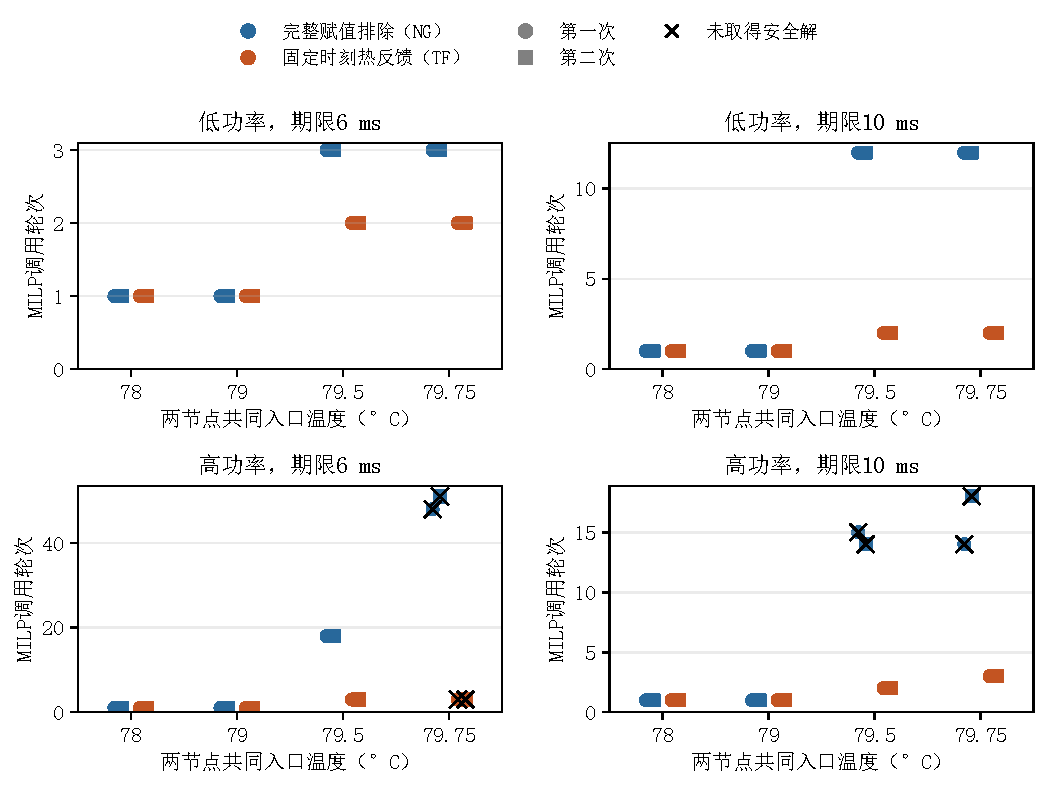
\includegraphics[width=\linewidth]{figures/pressure78_rounds.pdf}
\caption{预定入口热压力下两方法的MILP调用轮次。圆点、方点分别表示两次运行，叉号表示预算内没有安全输出；横向偏移只为避免遮挡。超时轮次是已发生的调用数，不表示搜索完成。各温度作为离散条件展示，不插值为连续区域边界。}
\label{fig:pressure-rounds}
\end{figure}

\clearpage

在每种方法的32次调用中，NG与TF分别取得26次和30次预算内安全输出，其中分别有12次和16次达到独立下界。双方均成功的26个配对所得能量全部相同，差异主要体现在安全输出次数与求解过程。低功率包79.5和79.75°C下的四个条件，以及高功率包6 ms、79.5°C条件，在两次运行中均减少求解轮次并缩短墙钟时间；其中，低功率包10 ms的两档高温条件均由12轮降至2轮。这五个条件下，两方法最终给出的时间表不同，说明相同能量仍可通过不同安全安排实现。

\begin{samepage}
高功率、10 ms、79.5与79.75°C两个条件中，NG四次调用均超时，未取得安全$U$；TF分别经过2轮和3轮取得42.625 mJ，并由$U=L_0$独立确定最优值。TF取得的安全见证同时确认了这些条件的可行性，NG则未能在本次预算内找到安全安排。这一差异体现的是有限预算下取得有效答案的能力；NG没有输出能量，因而这两个条件不能用于计算两方法之间的节能率。
\par
\end{samepage}

高功率、6 ms、79.75°C下，两方法均没有安全输出。NG两次超时；TF两次均加入两条热行，在完成3轮后由求解器报告无解。热行有效性保证安全安排得到保留，却不能独立认证浮点求解器已排尽剩余整数域。因此，该条件的结论仍为未取得安全输出与求解器报告无解，尚无独立热不可行证明；相应内部界和退出状态也与安全$U$、独立$L_0$分列报告。

较低入口提供了未触发反馈的对照。78与79°C的8个条件中，首候选均安全，两方法都只求解一轮且未执行反馈；对应16个配对中，TF恰有8次较快、8次较慢，这些时间差不能归因于未执行的热行。两档较高初温的8个条件中，首候选均违规；全部32个配对的首候选选项集合相同，排除了不同初始候选这一解释。两次顺序平衡运行支持本组观察的一致性，但不足以估计方差、置信区间或认定跨平台稳定加速。

求解过程进一步反映了两种反馈传递信息的差异。正式组中，NG共生成240条完整赋值排除，TF生成22条热行且无回退；累计求解轮次由272降至54，不同候选及完整热评价次数由282降至56。一轮求解可能在回调中访问多个候选，因而轮次与候选数分别统计。全部保存轮次的求解器分支节点计数均为0，减少的是外层重复求解，而非分支树节点。TF累计约束构造时间为0.602 s，高于NG的0.042 s；在触发反馈且双方成功的五个条件中，后续求解减少抵消了这项新增成本。

上述耗时采用完整调用的墙钟时间，首次取得安全输出的时间另以外部时刻区间记录，并以上端判断是否满足预算。NG六次超时调用实际在60.164--63.701 s返回，超出60 s的部分为停止延迟。完整墙钟保留了这一停止成本，预算内证据则仅接纳预算结束前完成检查的结果，未将晚形成的状态或内部界补记为有效输出；首次安全时间的区间下端也不作为精确首解时刻。

为检查已有违规轨迹能否在正常求解中触发反馈，另设高功率、6 ms、79.45°C的发现性诊断。该点依据既有轨迹构造，两方法各运行一次，均自主取得44 mJ安全输出：NG为18轮、24.826 s，TF为3轮、4.205 s。独立$L_0$仍为42.625 mJ，因此本项结果只提供安全见证与内部收敛。由于选点方式与正式温度组不同，诊断结果单独报告，不并入16个正式条件的成功率或重复统计。

离线检查表明，一条热行能够排除共享温度关系的多条违规安排；完整求解进一步表明，当较高入口使正常候选违规时，这种信息复用可以减少重复尝试，并在部分受预算限制的调用中取得安全最优值见证。该变化来自求解过程，能耗模型保持不变，双方均成功时也未观察到能量下降。结论适用于所列抽象参数、有限网格和求解器设置，不能据此推断真实设备节能或全部热调度实例的速度优势。


\subsection{结果讨论与适用范围}

本节结果分别回答了模型与方法的验证问题。任务响应修正的系统价值受期限和资源限制，温度约束可以收缩最优配置集合而不提高最低能量；在此模型上，连续温度违规信息能够形成有效线性约束，并在所测高入口条件下减少重复求解。表\ref{tab:evidence-map}汇总各项结论的求解来源和适用范围。

\begin{table}[htbp]
\centering\small
\caption{验证问题、求解来源与证据范围}\label{tab:evidence-map}
\setlength{\tabcolsep}{4pt}
\begin{tabular}{@{}p{2.2cm}p{2.5cm}p{4.4cm}p{4.7cm}@{}}
\toprule
验证问题 & 求解来源 & 已有证据 & 尚不能支持的结论\\
\midrule
响应修正是否改变决策 & 解析下界、排除及见证核验 & 宽期限有能量差，紧期限不变；覆盖反比模型并列解的回放能量 & 不是两种响应的MILP直接配对运行，也不是实测精度验证\\
温度是否限制配置 & 完整网格枚举 & 104个最优配置保留80个，最低仍44 mJ & 不推出最低能量提高或连续启动域的配置排除\\
热行是否利用更多信息 & 完整合法域离线核对 & 单行排除16或32条违规安排，零误删安全安排 & 排除数量本身不等于MILP加速\\
接入是否必然触发 & 原输入上独立MILP对照 & 9项可行输入均首轮安全，全部零反馈 & 不能由未触发时的耗时差判断反馈价值\\
反馈是否改善求解 & 16条件、两方法、两次运行 & 安全输出26/32与30/32；5条件轮次及时间减少，2条件仅反馈取得安全解 & 不证明普遍加速、运行能耗下降或创新充分成立\\
\bottomrule
\end{tabular}
\end{table}

本章方法将完整轨迹中已确认的违规节点与时刻转换为全部选项共同满足的温度必要条件，再通过可靠数值包络将其反馈给MILP。在线性热模型和约束生成思想的基础上，本章针对设备映射、频率与启动选项建立约束表达，论证有效性并验证求解表现。RC模型、查表和约束生成本身仍采用已有原理。与逐条删除当前安排相比，方法能否产生实际收益，取决于求解器是否遇到违规候选、不同候选是否共享温度关系，以及约束构造代价能否由后续求解减少抵消。

\begin{samepage}
各组输入、时间表、结果与求解来源的复现索引见随稿材料\cite{artifact-index}。其中，响应对照采用解析证据，尚未进行两种响应模型的MILP直接配对运行。第四章与有界搜索的比较应使用相同输入、预算和连续热接纳条件，并以加入热行反馈后的MILP为比较对象；此前针对完整赋值排除方法的比较不能替代这一检验。
\par\end{samepage}

本章结果的现实适用范围受参数来源限制。公开工件提供了四Stage结构及作者报告的设备支持，但目前缺少同平台Lite0各Stage的多频点时长、活动功率和配套RC测量。因此，实验分析的是声明条件下的决策关系，尚不能估计某款设备的实际节能率。冷热入口与期限对照也只覆盖所列条件，不能用于推断这些关系在现实系统中的出现频率。

能量分解的适用范围还取决于加性功率与固定模式响应。若并发改变活动功率或执行时长，或温度相关泄漏、休眠及切换代价使能量依赖具体安排，目标一般需恢复为$E(m,s)$。此时，一条安全时序不能确定整个配置的最低能量，独立Stage下界也须重新检查，尤其需要计入可能为负的并发修正。温度漏电与工作点保持已纳入第3.2—3.5节的一般模型，但其求解与验证不在本节结果范围内；并发残差、休眠和非零切换仍不属于本章基础假设。

\section{本章小结}

本章面向端侧协同多模型完整请求，建立设备、工作点与执行时序的热约束节能联合问题。合法模式提供任务相关代价，依赖、资源和共享域限定执行关系；功率按计量组去重，空闲工作点保持与温度漏电参与完整窗口能量。CPU固定单元及加速器设备的热状态通过耦合RC关联，完整安排的目标为\(E(m,s)\)。

在已实现的CPU--NPU恒功率特例上，本章保留有限网格MILP、连续热反馈及其验证。响应对照在宽期限下出现能量差，在紧期限下保留无变化条件；热约束收缩部分最优配置集合而未提高最低能量。预定热压力组中，安全输出由26/32次增至30/32次，共同成功时能量相同。这些结果对应原特例和输入，不替代一般模型的适配验证。

后续求解应围绕同一合法域与完整评价组织MILP参照和启发式，先处理工作点保持、漏电能量与多节点连续热检查的接口，再比较安全解质量和计算表现。

% 配置性质、热反馈推导与数值约定；在本章小结之后、符号索引之前载入。
\clearpage
\section*{补充性质与证明}
\label{sec:ch3-properties}
\markright{补充性质与证明}

本部分仅适用于第3.6—3.7节的恒功率、二聚合热节点特例；不将配置能量分解或固定选项热行推广为第3.2—3.5节一般模型的性质。

\subsection*{配置能量与时序可行性}

本部分说明配置能量与时序可行性的关系，并给出热约束影响最优配置及能耗的条件。模式中的映射与频率决定执行时长、活动能量、资源冲突和注热位置；时序决定这些选择能否组成满足全部要求的完整安排。两类决策的联系如图\ref{fig:config-timing}所示。

\begin{figure}[!htbp]
\centering
\resizebox{\linewidth}{!}{%
\begin{tikzpicture}[node distance=7mm and 10mm,box/.style={draw,rounded corners,align=center,text width=4.5cm,minimum height=10mm,font=\small},>=Latex]
\node[box] (d) {Stage模式表与合法支持};
\node[box,below=of d] (m) {配置$m$：执行单元与频率};
\node[box,below left=of m] (e) {固定配置能量$E(m)$};
\node[box,below right=of m] (s) {时序$s$：执行顺序与等待};
\node[box,below=of s] (r) {资源、频率域与请求期限};
\node[box,below=of e] (p) {配置与时序共同确定\par 完整节点功率轨迹$p(t)$};
\node[box,below=of p] (t) {入口状态与RC传播\par 连续热安全};
\node[box,below=of r] (f) {是否存在完整可行安排};
\node[box,below right=of t] (o) {选择最低可实现能量};
\draw[->] (d)--(m); \draw[->] (m)--(e); \draw[->] (m)--(s);
\draw[->] (s)--(r); \draw[->] (m.west) -| ([xshift=-4mm]p.west) -- (p.west);
\draw[->] (s)--(p); \draw[->] (p)--(t); \draw[->] (r)--(f);
\draw[->] (t)--(f); \draw[->] (f)--(o);
\draw[->] (e.west) -- ++(-10mm,0) |- (o.west);
\end{tikzpicture}%
}

\caption{配置能量与时序可行性的关系。图示为问题结构，不规定一次性的先配置后调度算法。}
\label{fig:config-timing}
\end{figure}

在上述特例的固定窗口、恒定基准功率、固定模式响应和零额外开销的条件下，每个Stage在窗口内完整执行一次，等待与重排不改变配置的总能量。因此，可以将“配置的代价是多少”与“该配置是否存在安全安排”分别描述。对固定配置\(m\)，记满足依赖、资源和期限等无热约束的启动向量集合为\(\mathcal S_0(m)\)，进一步满足温度约束的集合为\(\mathcal S_T(m)\)。存在相应时序的配置分别组成
\[
\mathcal M_0=\{m:\mathcal S_0(m)\ne\varnothing\},\qquad
\mathcal M_T=\{m:\mathcal S_T(m)\ne\varnothing\},
\]
\noindent\begin{minipage}{\linewidth}
\setlength{\parindent}{2em}
其中，所有配置均取自\(\prod_iM_i\)。以下集合与最优值均在相同启动域下比较。对于连续版本，时序集合允许连续起点；对于第\ref{sec:milp}节的网格版本，则统一限制到给定启动网格。联合问题可等价写为

\begin{equation}
\boxed{\min_{\substack{m\in\prod_{i\in V}M_i\\s\in\mathcal S_T(m)}}E(m)
=\min_{m\in\mathcal M_T}E(m).}
\label{eq:ch3-16}
\end{equation}

\textbf{命题3-1：} 式\eqref{eq:ch3-16}与联合问题具有相同的可实现目标值集合。

\textbf{证明：} 任意联合可行解\((m,s)\)中的配置都属于\(\mathcal M_T\)，能量为\(E(m)\)；反之，若\(m\in\mathcal M_T\)，则至少存在一条完整安全时序\(s\)，使\((m,s)\)成为联合可行解，能量同样为\(E(m)\)。两种表达取得的目标值集合因此相同。模式集合有限，\(\mathcal M_T\)非空时可取得其中最低能量；为空时则无完整可行安排。证毕。
\end{minipage}\par\medskip

该性质说明，找到一条满足全部约束的完整安排，就能证明其配置能量可以实现，即正文中所称的安全见证。一条时序失败则只排除了这一安排，判断整个配置不可行仍需覆盖其全部可能时序或给出充分排除依据。

温度要求对最优能耗的影响也可由此说明。设无热问题可行，其最优值为\(E_0^*=\min_{m\in\mathcal M_0}E(m)\)，最优配置集为\(\mathcal M_0^*=\{m\in\mathcal M_0:E(m)=E_0^*\}\)；若热问题也可行，记最优值为\(E_T^*\)。由于\(\mathcal M_T\subseteq\mathcal M_0\)，有

\begin{equation}
E_T^*\ge E_0^*,\qquad
E_T^*=E_0^*\ \Longleftrightarrow\ \mathcal M_T\cap\mathcal M_0^*\ne\varnothing.
\label{eq:ch3-17}
\end{equation}

只要原最优配置中还保留一个热可行配置，就能通过它的安全时序达到原最优值；反之，达到同一能量的热安全方案也必然来自这一交集。因此，最优配置集合缩小并不必然提高最低能耗。只有全部原最优配置被排除、但仍存在其他热可行配置时，有限配置集合才保证最优能量严格提高；若所有配置均被排除，则问题不可行。


\subsection*{选项热响应的展开}
\label{supp:option-response}

正文式\eqref{eq:thermal-affine}将节点温度分为基准与选项活动温升，此处给出各项的计算表达。在固定入口状态、线性时不变RC和可加活动功率下，每个选项的热响应可以分别独立计算。记全部选项为\(\mathcal O=\bigcup_{i\in V}\mathcal O_i\)，用热传播核描述温度状态随时间的变化：
\begin{equation}
K(t)=\exp(-C_{\rm th}^{-1}Gt),\qquad t\ge0.
\label{eq:thermal-kernel}
\end{equation}
温度基准由入口状态和持续的空闲注热产生，选项温升则由对应执行区间内的活动注热产生。设\(p^0=[p_C^0,p_N^0]^{\mathsf T}\)，\(\theta_0=\theta(0)\)。CPU模式选项\(o=(i,m,k)\)的活动注热向量为\(v_o=[Q_i(m),0]^{\mathsf T}\)，NPU模式则为\([0,Q_i(m)]^{\mathsf T}\)，单位均为W。边界外公共功率只计入系统能量，不进入\(p^0\)或\(v_o\)。由式\eqref{eq:ch3-14}，基准温度与选项响应分别为
\begin{equation}
\begin{aligned}
b_n(t)&=T_a+\left[K(t)\theta_0+
\int_0^t K(t-u)C_{\rm th}^{-1}p^0\,\mathrm du\right]_n,\\
h_{no}(t)&=
\begin{cases}
\displaystyle\left[\int_{t_o}^{\min(t,e_o)}
K(t-u)C_{\rm th}^{-1}v_o\,\mathrm du\right]_n,&t>t_o,\\
0,&t\le t_o.
\end{cases}
\end{aligned}
\label{eq:thermal-option-response}
\end{equation}
其中，\(b_n\)为包含初温和固定空闲注热的绝对温度，单位为°C；\(h_{no}\)为活动温升，单位为K，其数值可与°C温差相加。选项尚未启动时，活动温升为零；执行结束后，已有温升仍随热传播变化。因此，\(h_{no}\)同时取决于注热节点、执行区间和观察时刻，与只表示功率积分的活动能量\(\varepsilon_o\)承担不同作用。

本特例的被动RC网络中，\(-C_{\rm th}^{-1}G\)的非对角元素非负，因而\(K(t)\)逐元素非负；结合\(v_o\ge0\)，可得\(h_{no}(t)\ge0\)。上述系数依赖选项响应的独立性；若加入温度相关泄漏，或并发改变选项时长与功率，则需重新审查这种表达。


\subsection*{热反馈的有效性与覆盖关系}
\label{supp:feedback-properties}

将热演化与调度联合写入MILP已有研究基础。Pierson等采用离散时间热模型建立资源分配与能量优化约束\cite{pierson2020}；本章则在连续耦合RC模型下，依据完整轨迹的违规位置生成约束。有限主问题与违规分离交替进行的组织方式可借鉴Subramanyam等的研究\cite{subramanyam2020}，约束有效性及终止条件仍需按本问题的假设推导，其收敛结论不能直接移用。

正文中的反馈行采用响应下界与放宽右端，并对源候选验证严格分离。下面分别说明这两项条件所保证的安全保留与排除范围。

\noindent\begin{minipage}{\linewidth}
\setlength{\parindent}{2em}
\textbf{命题3-2：} 式\eqref{eq:thermal-safe-row}保留全部原热安全安排。

\textbf{证明：} 若安排违反该行，由\(y_o\ge0\)及响应下界可得
\begin{equation}
T_n(\bar t;y)\ge\underline b_n+\sum_o a_oy_o
>\underline b_n+r\ge T_n^{\max}+\epsilon_T.
\label{eq:thermal-row-validity}
\end{equation}
故被排除安排必然超温，不属于原热安全集合。放宽右端只会减小排除范围，不会改变最终安全接纳标准。\hfill$\square$
\end{minipage}\par\medskip

\textbf{命题3-3：} 在满足逐Stage唯一选择的合法整数域中，若式\eqref{eq:thermal-source-separation}成立，则热行保留的安排集合包含于对应完整赋值排除保留的集合。

\textbf{证明：} 完整赋值排除只删除同时选择\(J^*\)中全部\(N\)个选项的安排，唯一选择约束保证该安排就是源安排。式\eqref{eq:thermal-source-separation}保证源安排也被热行删除，故满足热行的整数安排必满足对应完整赋值排除。\hfill$\square$

只有存在另一个同样违反该热行的合法整数安排时，上述包含关系才严格。命题说明违规温度信息可以用于排除其他安排，其范围限于满足唯一选择约束的合法整数域；分数解上的支配关系及实际求解加速仍需分别研究。

上述两项条件也给出有限域内的终止依据。假设主问题精确求解，连续热判定能够按原温度约束将每个候选明确分为安全或违规，不存在未分辨状态；若每轮新增约束全域有效，并严格排除当前违规候选，该候选便不会再次出现。选项域有限，因此在预算不限时，反馈经过有限轮次必得到安全安排或排空合法域。进一步，若每轮返回当前松弛问题的真正最优解，首次被接纳的安全解就是原有限网格热问题的最优解：松弛最优值提供下界，该安全解提供相同的可行上界。

实际求解的停止结论还取决于数值判定与计算预算。响应系数和连续峰温包络的数值保证均限于已核对的对称二节点实现；一般RC线性关系本身不提供任意网络的数值认证。求解过程分别保存安全\(U\)、独立\(L_0\)、求解器内部界及未决状态，有效热行也不独立认证求解器内部界。因此，超时、未分辨或主问题未收敛时，结果仍按已取得的证据报告，不能由有限域终止论证推定搜索已经完成。


\subsection*{数值复核与实现约定}
\label{supp:numerical-checks}
\enlargethispage{\baselineskip}

峰温误差包络与判定带宽承担不同作用：前者控制峰温计算误差，后者区分接近阈值的情况。对系数、右端与求和也需分别采用可靠包络，不能仅将温度容差视作计算误差保证。式\eqref{eq:thermal-safe-row}采用非负响应下界，放宽右端会减小排除范围，但不改变最终安全接纳标准。

完整轨迹已证违规后，名义峰时刻只用于定位。实现需在具体可表示时刻重新构造点证书，并对源候选的被选集合\(J^*\)计算可靠求和下界，验证式\eqref{eq:thermal-source-separation}。全局峰温下界不能代替某个时刻的点温度下界，普通浮点和略大于右端也不能作为严格分离证据。完整轨迹违规但点证书或分离条件未成立时，回退式\eqref{eq:no-good}；轨迹未分辨时，两种排除均不生成。

检查器先按指定整数容差解码近整数候选，再根据真实区间复核唯一选择、依赖、资源和频率域要求。整数结构约束与浮点热行分开检查，热行采用可靠区间求和。解码或结构复核失败记为数值异常，不接纳候选，也不据此生成热排除。

一次调用按完整选项集合识别缓存候选，可复用完全相同候选的热检查结果；加入新热行后，仍需重新检查其是否满足当前约束。热行按完整系数向量及右端的精确相等识别重复，只保留一条。重复行不构成新进展；再次返回已被热行明确排除的违规候选时，记录容差事件并改用该完整赋值的排除。若候选还违反已加入的整数排除约束，则停止为数值异常，不反复重启。

热行检查与完整轨迹检查保持一致：热行比较未分辨、完整轨迹已证安全时，可依据完整检查保存安全\(U\)；若达到\(U=L_0\)，仍可独立证明最优值。未达到独立上下界闭合且最终热行比较仍未分辨时，停止为数值未决。热行明确违规而完整轨迹被判安全时，记录矛盾并停止为异常。实现错误不作为正常回退处理。

有限网格的安全安排也是连续启动问题的安全安排；网格最优或不可行结论则限于该受限域。只有连续域有效下界被某个网格安全安排达到时，才能进一步确定连续域最优值。\(L_0\)的独立Stage构造对两种域均成立，使用时仍须确认各模式集非空，并区分最优值与全部最优配置集合。


% 当前多场景模型的章末索引。
\clearpage
\section*{本章符号索引}
\markright{本章符号索引}

各符号在正文首次使用处定义。本表按输入、决策与派生量归类，内部时间、频率、功率和能量单位分别为s、Hz、W和J；温度使用摄氏温标，温差使用K。

\begin{longtable}{@{}p{5.1cm}p{6.1cm}>{\raggedright\arraybackslash}p{2.8cm}@{}}
\caption{多场景联合规划的主要符号}\label{tab:symbols}\\
\toprule
符号 & 含义 & 类型／单位 \\
\midrule
\endfirsthead
\toprule
符号 & 含义 & 类型／单位 \\
\midrule
\endhead
\(\mathcal A,G_a,V_a,E_a\) & 应用及其固定Stage工作流 & 输入集合／图 \\
\(\mathcal C,\mathcal R_c,\mathcal I_c,\mathcal E_c\) & 场景、请求、Stage实例及依赖 & 输入集合 \\
\(\mathcal J,\tau(c,i),r(c,i),\mathcal O_{cr}\) & 固定Stage身份、实例归属及必需输出 & 输入集合／映射 \\
\(r_{cr},d^{\rm rel}_{cr},D_{cr},W_c\) & 释放、相对期限、绝对期限及窗口 & 输入，s \\
\(p_c\) & 完整场景片段的次数权重 & 输入，无量纲 \\
\(\mathcal U_C,\mathcal U_G,\mathcal U_N\) & CPU固定单元、GPU及NPU设备 & 输入集合 \\
\(\mathcal H,\gamma(u),\mathcal K_h\) & 控制域、单元归属及合法工作点 & 输入集合／映射 \\
\(f_h(k),v_h(k),k^0_{ch}\) & 工作点频率、电压及入口状态 & Hz、V、状态标签 \\
\(\mathcal M_{ci},u(m),\kappa(m)\) & 合法模式、对应单元及完整域工作点 & 输入集合／映射 \\
\(d^{\rm ref}_{\tau u},f^{\rm ref}_u,\alpha_{\tau u}\) & 参考时长、参考频率及可缩放比例 & s、Hz、无量纲 \\
\(d_\tau(m),q_\tau(m)\) & 模式时长及活动增量功率 & 派生／输入，s、W \\
\(\mathcal B,\pi(u),\xi_{cg}(t)\) & 计量组、单元归属及组控制状态 & 输入／派生 \\
\(B_g,\lambda_{gn},T_g^{\rm ref}\) & 参考基准、本地温度系数及参考温度 & W、W/K、摄氏度 \\
\(a^B_{ng},n(u),h_{nu}\) & 基准分布、单元节点及活动注热映射 & 输入，无量纲／映射 \\
\(\mathcal N,C,G,T_a,T_c^0,T_n^{\max}\) & 热节点、热容、导热及温度输入 & J/K、W/K、摄氏度 \\
\(P_{{\rm ext},c},E_{{\rm ext},c}\) & 给定边界外功率及其窗口能量 & W、J \\
\midrule
\(u_\tau,m_{ci},s_{ci}\) & 共享部署、实例模式及启动时刻 & 共同／场景内决策 \\
\(F_{ci},I_{ci},\iota_{ci},k_{ch}(t)\) & 完成、执行区间、活动及域轨迹 & 派生，s／0--1／标签 \\
\(P_{cg},p^{\rm heat}_{cn},\theta_c,E_c,\bar E\) & 组电功率、注热、温升及能量 & W、K、J \\
\midrule
\(\mathcal G_{cim},\mathcal Q_{ci},\mathcal Q_c\) & 有限启动集合与单Stage选项 & 输入／派生集合 \\
\(t_o,f_o,d_o,q_o,u_o,h_o,\kappa_o\) & 选项的起止、代价及资源控制要求 & 已知选项参数 \\
\(e_{c\ell},\delta_{c\ell},\chi_{co\ell}\) & 固定事件、片长及半开区间覆盖 & 已知，s、0/1 \\
\(x_{\tau u},y_{co}\) & 共享部署和选项选择 & 二元变量 \\
\(\rho_{ch\ell k},w_{c\ell\omega}\) & 域状态及相容联合状态选择 & 二元辅助变量 \\
\(\Omega,J_{ch\ell},v_{c\ell}\) & 联合状态集、新启动数量及活动向量 & 输入／派生 \\
\(\theta_{c\ell},\Delta E_{c\ell}\) & 事件温升及完整段能量 & 连续变量，K、J \\
\(A_\omega,b_\omega,D_c,\beta_\omega,\ell_\omega\) & 固定状态下的热与电功率系数 & 由物理输入派生 \\
\(\Phi,\psi,\Gamma,\mu,\zeta,\nu\) & 温度传播及能量积分系数 & 由状态／片长派生 \\
\(H_c,\overline P_c,M^T,M^E\) & 状态、功率及条件行残差界 & 有依据的派生界 \\
\(\mathcal H^{(j)},U\) & 已加入的必要行及安全能量上界 & 求解记录，J \\
\bottomrule
\end{longtable}


% 第四章尚未撰写正文。完成后在此加入 \input{chapter04}。
\begin{thebibliography}{99}
\bibitem{kim2023scenario}
Kim J, Ha S.
Energy-Aware Scenario-Based Mapping of Deep Learning Applications Onto Heterogeneous Processors Under Real-Time Constraints[J].
IEEE Transactions on Computers, 2023, 72(6): 1666--1680.
\url{https://doi.org/10.1109/TC.2022.3218991}.
\bibitem{chantem2011}
Chantem T, Hu X S, Dick R P.
Temperature-Aware Scheduling and Assignment for Hard Real-Time Applications on MPSoCs[J].
IEEE Transactions on Very Large Scale Integration (VLSI) Systems, 2011, 19(10): 1884--1897.
\url{https://doi.org/10.1109/TVLSI.2010.2058873}.
\bibitem{source1}
Zhou J, Yan J, Cao K, et al.
Thermal-aware correlated two-level scheduling of real-time tasks with reduced processor energy on heterogeneous MPSoCs[J].
Journal of Systems Architecture, 2018, 82: 1--11.
\bibitem{source2}
Da Costa G.
Hardware and application aware performance, power and energy models for modern HPC servers with DVFS[J].
Sustainable Computing: Informatics and Systems, 2025, 46: 101106.
\url{https://doi.org/10.1016/j.suscom.2025.101106}.
\bibitem{fdtm2022}
Maity S, Roy R, Majumder A, Dey S, Hota A R.
Future aware Dynamic Thermal Management in CPU-GPU Embedded Platforms[C]//2022 IEEE Real-Time Systems Symposium (RTSS).
2022: 396--408.
\url{https://doi.org/10.1109/RTSS55097.2022.00041}.
\end{thebibliography}
\end{document}
